% !TeX root = bbchallenge-paper.tex

\title{Determination of the fifth Busy Beaver value}
\author{
        bbchallenge's contributors
}

\documentclass[a4paper,british]{article}

\usepackage{babel}
\usepackage[utf8]{inputenc}
\usepackage[margin=1in]{geometry}
%\usepackage{subfig}
\usepackage[hidelinks]{hyperref}
\usepackage{caption}
\usepackage{floatpag}
\usepackage{subcaption}
\usepackage{tikz}

\usepackage{algorithm}
\usepackage[noend]{algpseudocode}
\usepackage{xcolor,colortbl,tikz}

\usepackage{bold-extra}% bold texttt

\usepackage{graphicx}
\usepackage{mathtools}

\usepackage{booktabs} 

\usepackage{amsmath,amsfonts,amssymb,amsthm}

\theoremstyle{definition} % don't use italics
\newtheorem{theorem}{Theorem}[section]
\newtheorem{definition}{Definition}[section]
\newtheorem{lemma}{Lemma}[section]
\newtheorem{proposition}{Proposition}[section]
\newtheorem{corollary}{Corollary}[section]
\numberwithin{equation}{section}


\theoremstyle{definition} % emphasize the "Remark N." with italics, not bold
\newtheorem{observation}{Observation}[section]
\newtheorem{example}{Example}[section]
\newtheorem{remark}{Remark}[section]

\usepackage{xassoccnt}
\DeclareCoupledCountersGroup{theorems}
\DeclareCoupledCounters[name=theorems]{theorem,definition,lemma,proposition,corollary,remark,observation,example}

\usepackage{microtype,xspace,wrapfig,multicol} 
\usepackage[textsize=tiny,color=lightgray]{todonotes} 
\usepackage[normalem]{ulem} % sout
\usepackage{stmaryrd}


\newcommand{\ts}[1]{{\color{red}#1}}
\newcommand{\tsi}[1]{\todo[inline]{TS: #1}}
\newcommand{\tsm}[1]{\todo{TS: #1}}
\newcommand{\tss}[2]{{\ts{\sout{#1}}} {\ts{#2}}}
\newcommand{\jb}[1]{{\color{blue}#1}}
\newcommand{\jbi}[1]{\todo[inline]{JB: #1}}
\newcommand{\jbm}[1]{\todo{JB: #1}}
\newcommand{\jbs}[2]{{\jb{\sout{#1}}} {\jb{#2}}}
\newcommand{\tabi}{\hspace{\algorithmicindent}}
\newcommand{\Lim}[1]{\raisebox{0.5ex}{\scalebox{0.8}{$\displaystyle \lim_{#1}\;$}}}
\newcommand{\N}{\mathbb{N}}
\newcommand{\Z}{\mathbb{Z}}

\newcommand{\lhead}[1]{\stackrel{#1}\triangleleft}
\newcommand{\rhead}[1]{\stackrel{#1}\triangleright}

\newcommand{\tm}[1]{\href{https://bbchallenge.org/#1}{\nolinkurl{#1}}}

\usepackage{xcolor}

\definecolor{colorA}{RGB}{255,0,0}
\definecolor{colorB}{RGB}{255,128,0}
\definecolor{colorC}{RGB}{0,0,255}
\definecolor{colorD}{RGB}{0,255,0}
\definecolor{colorE}{RGB}{255,0,255}

\newcommand{\stateA}{{\textcolor{colorA}{A}}\xspace}
\newcommand{\stateB}{{\textcolor{colorB}{B}}\xspace}
\newcommand{\stateC}{{\textcolor{colorC}{C}}\xspace}
\newcommand{\stateD}{{\textcolor{colorD}{D}}\xspace}
\newcommand{\stateE}{{\textcolor{colorE}{E}}\xspace}

\newcommand{\szero}{\texttt{0}\xspace}
\newcommand{\sone}{\texttt{1}\xspace}

\def\@fnsymbol#1{\ensuremath{\ifcase#1\or *\or \dagger\or \ddagger\or
   \mathsection\or \mathparagraph\or \|\or **\or \dagger\dagger
   \or \ddagger\ddagger \else\@ctrerr\fi}}
\newcommand{\ssymbol}[1]{^{\@fnsymbol{#1}}}

\newcommand{\BBtheFourth}{107}
\newcommand{\SigmaTheFourth}{13}
\newcommand{\BBtheFourthTNF}{858{,}909}

\newcommand{\BBtheFifth}{47{,}176{,}870}
\newcommand{\BBtheFifthTNF}{181{,}385{,}789}
\newcommand{\SigmaTheFifth}{4{,}098}

\newcommand{\BBTxF}{3{,}932{,}974}
\newcommand{\BBTxFTNF}{2{,}154{,}217}

\newcommand{\radofull}{Tibor Rad\'o\xspace}
\newcommand{\rado}{Rad\'o\xspace}

\newcommand{\cryptid}{Cryptid\xspace}

\newcommand{\cycler}{Cycler\xspace}
\newcommand{\cyclers}{Cyclers\xspace}
\newcommand{\TC}{Translated Cycler\xspace}
\newcommand{\TCs}{Translated Cyclers\xspace}

\newcommand{\headpos}{head-position\xspace}
\newcommand{\headposs}{head-positions\xspace}

\newcommand{\states}{\mathcal{S}}
\newcommand{\alphabet}{\mathcal{A}}
\newcommand{\symbolzero}{\texttt{0}}
\newcommand{\symbolone}{\texttt{1}}

\newcommand{\numSporadic}{13\xspace}

\newcommand{\ssp}{state-symbol-pair\xspace}
\newcommand{\ssps}{state-symbol-pairs\xspace}

\newcommand{\HALT}{\texttt{HALT}\xspace}
\newcommand{\NONHALT}{\texttt{NONHALT}\xspace}
\newcommand{\UNKNOWN}{\texttt{UNKNOWN}\xspace}

\newcommand{\CoqBB}{Coq-BB5\xspace}
\newcommand{\CoqBBnospace}{Coq-BB5}

\newcommand{\TMstep}{\to}

\begin{document}
\date{}
\maketitle

\begin{abstract}
    ee
\end{abstract}


\setcounter{tocdepth}{2}
\tableofcontents
\newpage

\begin{center}

\end{center}



\begin{figure}
    \begin{quote}
        ``In any case, even though skilled mathematicians and experienced programmers attempted to evaluate $\Sigma(3)$ and S(3), there is no evidence that any known approach will yield the answer, even if we avail ourselves of high-speed computers and elaborate programs. As regards $\Sigma(4)$, $S(4)$ the situation seems to be entirely hopeless at present.'' --- \radofull, 1963 \cite{Rado_1963}
    \end{quote}
    \begin{quote}
        ``\textit{Prediction 5}. It will never be proved that $\Sigma(5) = \SigmaTheFifth$ and $S(5) = \BBtheFifth$.'' --- Allen H. Brady, 1990 \cite{BradyMeaningOfLife}
    \end{quote}
    \caption{\radofull, who invented the Busy Beaver game, proved the value of $S(2)$ in 1962 \cite{Rado_1962}, and was involved in the proof of $S(3)$ in 1963 \cite{Lin1963}, did not believe that $S(4)$ could be solved at his time. Allen H. Brady, who proved the value of $S(4)$ in 1983 \cite{Brady83}, did not believe that $S(5)$ could be solved at all. Amusingly, Brady opens his article on $S(4)$ with \rado's above quote \cite{Brady83}. Under that light, the knowledge of a (small) Busy Beaver value seems to be a reflection of the computing technology available at the time it was proved.}
\end{figure}

\vspace{-40pt}

\section{Introduction}

\subsection{Main Results}\label{sec:intro:mainresults}

\newcommand{\noncomput}{noncomputable\xspace}
\newcommand{\BBfull}{Busy Beaver\xspace}
\newcommand{\Coq}{Coq\xspace}
% We'll update this link to v1 release URL
\newcommand{\CoqProofReleaseURL}{\url{https://github.com/ccz181078/Coq-BB5}}

\newcommand{\ie}{i.e.~}
\newcommand{\eg}{e.g.~}

Are there simple \noncomput functions? What is the \textit{smallest} open problem in mathematics? What do algorithms look like, \textit{in the wild}?

Introduced by \radofull in 1962, \textit{the \BBfull game} gives a framework to answer these seemingly independent questions, starting with the first one since \rado's goal was to ``present some very simple instances of \noncomput functions'' \cite{Rado_1962}. The game is as such: (i) run all $n$-state Turing machines\footnote{See Appendix~\ref{app:TMs} for Turing machines definitions and examples.} from the all-zero tape (ii) consider the set of machines that eventually halt (iii) the winner of the game is the halting machine that has the most \sone symbols on its tape when it halts. This maximum number of \sone symbols on halting tape among $n$-state machines is called $\Sigma(n)$. \rado also introduced $S(n)$, the maximum number of steps made by a halting $n$-state Turing machine from all-zero tape. Both functions $\Sigma$ and $S$ are \noncomput! This is most obvious in the case of $S$: if an $n$-state machine runs for more than $S(n)+1$ steps, we know it will never halt, giving an algorithm to decide Turing's halting problem if $S$ was computable. This tight link between $S$ and the halting problem makes it more interesting and practical to us than $\Sigma$, hence we take the liberty to concentrate more on $S$.

%This tight link to the halting problem makes $S$ more interesting and practical to us than $\Sigma$, hence we take the liberty (similarly to other authors \cite{BusyBeaverFrontier,otherexamples?}) to focus the busy beaver game on $S$ instead of $\Sigma$ and to call the $n$-state \textit{busy beaver winner} the machine achieving $S(n)$ running steps. 
While there is no algorithm to compute $S(n)$ for \textit{all} $n$ we can certainly try to compute $S(n)$ for \textit{some} $n$. Prior to this work, only the four first values of $S$ had been proved: $S(1)=1$, $S(2)=6$ \cite{Rado_1962}, $S(3) = 21$ \cite{Lin1963}, $S(4) = 107$ \cite{Brady83}. With some early attempts in the 1960s and 1970s, the $S(5)$ quest seriously started in 1983 with a 2-day competition organised at the University of Dortmund\footnote{Report of the competition: \url{https://docs.bbchallenge.org/other/lud20.pdf}.} with the sole goal of finding new 5-state champions -- \ie 5-state machines achieving better $S$ scores than any machines previously known \cite{PMichel_website,michel2019busy}. The winning machine in Dortmund achieved $134,467$ steps, establishing $S(5) \geq 134,467$. In 1989, a big step was made when Marxen and Buntrock found a new champion achieving $\BBtheFifth$ steps \cite{Marxen_1990}, showing $S(5) \geq \BBtheFifth$; this machine is given in Figure~\ref{fig:bb5}. However, it remained unknown if no other machine could beat it, \ie whether Marxen and Buntrock's machine was the actual 5-state Busy Beaver winner or not. In 2020, Aaronson conjectured that there was no better 5-state machine, \ie $S(5) = \BBtheFifth$ \cite{BusyBeaverFrontier}.

Our main result is to prove this conjecture, using the \Coq proof assistant \cite{the_coq_development_team_2024_14542673}, see Theorem~\ref{th:BB5}. The winning machine for $S(5)$ is also the winning machine for $\Sigma(5)$. We also prove $\Sigma(5) = \SigmaTheFifth$, see Theorem~\ref{th:BB5Sigma}.

\begin{theorem}\label{th:BB5}
    $S(5) = \BBtheFifth$.
\end{theorem}

The function $S$ can naturally be extended to Turing machines using more than two alphabet symbols \cite{BradyMeaningOfLife}, like, for instance, $S(2,3) = 38$ is the value of $S$ for 2-state, 3-symbol machines \cite{BradyMeaningOfLife, MICHEL200445, LafittePapazian2007}. We prove, using Coq, that $S(2,4) = \BBTxF$, see Theorem~\ref{th:BB2x4} and Figure~\ref{fig:bb2x4}:

\begin{theorem}\label{th:BB2x4}
    $S(2,4) = \BBTxF$.
\end{theorem}

The Coq proofs for $S(5)$ and $S(2,4)$ --- as well as for previously known $S(2),\,S(3),\,S(4)$ and $S(2,3)$ --- are available at \url{https://github.com/ccz181078/Coq-BB5}. The lists of all the Turing machines evaluated by these proofs are available at \url{https://docs.bbchallenge.org/CoqBB5_release_v1.0.0/}.

The goal of this paper is to present these proofs. As a result of our work, we now have a clearer view of the landscape of small Busy Beaver values, see Table~\ref{table:landscape}.


\setlength{\fboxrule}{1.2pt}
\begin{table}[h]
    \centering
    \small
    \renewcommand{\arraystretch}{1.3}
    \setlength{\tabcolsep}{5pt}  % Adjust column spacing
    \begin{tabular}{c|ccccc}
        \hline
        \textbf{Symbols} & \textbf{2-State}                                                           & \textbf{3-State} & \textbf{4-State} & \textbf{5-State} & \textbf{6-State} \\
        \hline
        2                & \cellcolor{green!20}$S(2) = 6$ \cite{Rado_1962}
                         & \cellcolor{green!20}$S(3) = 21$ \cite{Lin1963}
                         & \cellcolor{green!20}$S(4) = 107$ \cite{Brady83}
                         & \cellcolor{green!50}{$S(5) = \BBtheFifth$}
                         & \cellcolor{orange!50}{$S(6) > 10 \uparrow \uparrow 15$}                                                                                                \\
        \hline
        3                & \cellcolor{green!20}$S(2,3) = 38$ \cite{LafittePapazian2007}
                         & \cellcolor{orange!50}{$S(3,3) > 10^{17}$}
                         & \cellcolor{orange!20}$S(4,3) > 2 \uparrow \uparrow \uparrow 2^{2^{{32}}} $
                         & --                                                                         & --                                                                        \\
        \hline
        4                & \cellcolor{green!50}{$S(2,4) = \BBTxF$}
                         & \cellcolor{orange!20}$S(3,4) > 2 \uparrow^{15} 5 $
                         & --                                                                         & --               & --                                                     \\
        \hline
        5                & \cellcolor{orange!50}{$S(2,5) > 10 \uparrow \uparrow 4$}
                         & --                                                                         & --               & --               & --                                  \\
        \hline
    \end{tabular}
    \caption{Landscape of small busy beaver values.
        \cellcolor{green!20}Cells highlighted in green correspond to values for which we provide \Coq proofs. Bright green indicates the new results, $S(5)$ and $S(2,4)$, original to this work.
        Cells highlighted in orange indicate the existence of a Cryptid (\ie machines whose halting problem is currently open and believed to be mathematically hard), see Appendix~\ref{app:cryptids}. Lighter orange means that the existence of a Cryptid comes trivially from reusing a known 3-state 3-symbol Cryptid and ignoring the available additional state or symbol. }
    \label{table:landscape}
\end{table}











\paragraph{Challenges.} Proving $S(5) = \BBtheFifth$ required analyzing the behavior of $\BBtheFifthTNF$ Turing machines\footnote{This exact number can only be known after the proof is done, see Section~\ref{sec:enum}.}-- evidently requiring computer assistance. The challenge for a halting machine is the case where it halts after a number of steps that is too enormous to be simulated step-by-step (e.g. the current 6-state champion halts after $10 \uparrow \uparrow 15$ steps \cite{Pavel_discorvery}, see Appendix~\ref{app:lowerbounds}), this challenge was not met for 5-state machines since they halt in at most $\BBtheFifth$ steps -- this could not have been known for certain in advance but was believed -- which is easy to simulate on modern computers. The challenge for a non-halting machine is that proving it does not halt can be hard. How hard?

Dauntingly, any $\Pi_1^0$ mathematical statement\footnote{A $\Pi_1^0$ statement is a statement of first-order logic of the form ``$\forall x, \phi(x)$'' where $\phi$ is a sentence with only bounded quantifiers (\ie $\phi(x)$ can always be verified by a computer in finite time).} can be encoded as the halting problem of a Turing machine (from all-zero tape). Such statements are common and include famous open problems in mathematics such as Goldbach's conjecture or the Riemann hypothesis. Goldbach's conjecture, formulated in 1742, is one of the oldest open problems in mathematics and states ``every even positive integer greater than 2 is the sum of two prime numbers.'' We can build a Turing machine that halts iff the conjecture is false: by enumerating all positive integers, then for each, test all sums of smaller primes and halt iff we do not find the sum. A (formally verified) machine performing this procedure has been built using only 25 states \cite{GoldbachTM27, GoldbachTM25}. This means that proving the value of $S(25)$ is at least as hard as solving Goldbach's conjecture because the proof of $S(25)$ must contain an argument as of why this particular 25-state machine does not (or, believed less likely, does) halt. Similarly, the Riemann hypothesis has been encoded in a 744-state machine \cite{RiemannTM,Yedidia2016,BusyBeaverFrontier}. As low as 15 states is enough to encode a hard number theoretical conjecture by Erd\H{o}s \cite{BB15}. Worst, the consistency of common axioms sets such as Peano's Arithmetic (PA) or Zermelo–Fraenkel set theory (ZF) is also $\Pi_1^0$ since one can enumerate proofs in these systems until the proof of a contradiction is found. This has been done for ZF, using 748 states \cite{ZFTM,Yedidia2016,BusyBeaverFrontier,BB748Thesis}. By G\"odel's second incompleteness theorem, this means that proving the value of $S(748)$ cannot be done using ZF. Aaronson conjectures that as low as $S(20)$ cannot be proven in ZF and as low as $S(10)$ cannot be proven in PA \cite{BusyBeaverFrontier}.

Hence, while 5-state halting machines were not feared, it remained unknown how hard non-halting 5-state machines could get. This article settles the question: the smallest open problem in mathematics (on the Busy Beaver scale) does not arise from 5-state machines -- but we have good contenders for 6-state machines, see Section~\ref{sec:cryptids}.

\paragraph{Related Work.} The proof of $S(4) = \BBtheFourth$ was published in 1983 \cite{Brady83}. One of its main innovations was the introduction of a method to solve the halting problem of a category of machines the author calls \textit{XMas Trees}. A caveat of \cite{Brady83} resides in the following quote from the paper: ``All of the remaining holdouts were examined by means of voluminous printouts of their histories along with some program extracted features. It was determined to the author's satisfaction that none of these machines will ever stop.'' A \textit{holdout} is a machine still needing a proof of halting/nonhalting. Using Coq, we bring additional confirmation that $S(4) = \BBtheFourth$, see Theorem~\ref{th:BB4}.

\newcommand{\SkeletHoldoutsSporadic}{\ts{XX}\xspace}

We know of two attempts at solving $S(5)$: in 2003, Georgi Georgiev (also known under pseudonym ``Skelet'' or ``Skeleta'') published the program \texttt{bbfind} \cite{Skelet_bbfind} which enumerates and decides the halting behavior of 5-state Turing machines, claiming to leave unsolved mainly 43 holdouts\footnote{\url{https://skelet.ludost.net/bb/nreg.html} and \url{https://bbchallenge.org/skelet}}. Attesting to the validity of the result is difficult as Skelet's code consists of ca. 6000 lines of uncommented and undocumented Pascal. That said, it turned out to be instrumental for our result as, after reverse engineering parts of it, we were able to learn and improve on his ``Closed Position Set'' technique (see Section~\ref{sec:n-gramCPS}) which improvements decided slightly more than 99.87\% of the 5-state Turing machines excluding loops (see Section~\ref{sec:loops}). All of our \numSporadic \textit{Sporadic Machines}, \ie machines for which we needed individual proofs of nonhalting, were either among Skelet's 43 holdouts or claimed to have been manually solved by him. See Section~\ref{sec:sporadic} for more discussion on our analyses of these longstanding holdouts. Some of Skelet's list of 43 holdouts were analysed by hand prior to our work \cite{DanBriggs}. The second known attempt at $S(5)$ was in 2008 with Hertel's ``Symbolic induction prover'', which claimed to leave only $1{,}000$ holdouts, $900$ of which were manually proven not to halt, allegedly leaving only $100$ proper holdouts \cite{Hertel}. In an opposite way to Skelet's work, the method is documented but, to the best of our knowledge, no code is made available, nor are the 900 claimed manual proofs, making verification of the result difficult apart from reproduction from scratch (arguably, verification would still be tedious if the 900 proofs were given).

The \BBfull problem was also studied in other models of computation than \rado's (c.f. Appendix~\ref{app:TMs}), including the \textit{quadruple} variation of Turing machines where each transition may move or write a new symbol, but not both \cite{Ross2003,Ross2005}. For additional historical perspective on the \BBfull problem, we refer the reader to Michel's survey and website \cite{michel2019busy,PMichel_website}.

\paragraph{Structure of the proof: overview.} Machines are enumerated arborescently in \textit{Tree Normal Form} (TNF) \cite{Brady64} which drastically reduces the search space's size -- \eg from ca. 10 trillion machines to $\BBtheFifthTNF$ for 5-state machines, see Section~\ref{sec:enum}.

Each enumerated machine is fed through a sequence (or \textit{pipeline}) of \textit{deciders}, where a decider is an algorithm trying to decide whether the machine halts or not. Because of the noncomputability of the halting problem, there is no \textit{universal} decider but all the craft resides in creating deciders able to decide large families of machines, in reasonable time. The $S(5)$ pipeline of deciders is given in Table~\ref{tab:pipelineBB5} -- see Tab~\ref{tab:pipelineBB2x4} for $S(2,4)$. Deciders are presented in Section~\ref{sec:deciders}. To the best of our knowledge, all the deciders we present are original.

In the case of 5-state machines, \numSporadic \textit{Sporadic Machines} were not solved by deciders and required individual proofs of nonhalting, see Section~\ref{sec:sporadic}. These machines include suprising behaviours, such as eventually-repeating chaos (machine ``Skelet \#1''), base-Fibonacci counters (machine ``Skelet \#10''), or obfuscated Gray code (machine ``Skelet \#17'', \cite{xu2024skelet17fifthbusy}) and they are beautiful examples of \textit{algorithms in the wild}: non-human-engineered algorithms that, like deep sea life, were only found by means of exploration.

\paragraph{Collaboratively solving the problem: bbchallenge.org.} In 2022, Stérin created ``The Busy Beaver Challenge'', \url{bbchallenge.org}, an online platform dedicated to collaboratively solving ``$S(5)=\BBtheFifth$'' \cite{sterin_2022_14955828}. Collaboration was motivated by the great amount of Turing machines to study in order to solve the problem. The bbchallenge platform essentially consists of the website, an instant chat server\footnote{\url{https://discord.gg/3uqtPJA9Uv}}, and, a wiki\footnote{\url{wiki.bbchallenge.org}}. The website serves as an entry-point to the problem and was providing a browsable \textit{seed database}\footnote{\url{https://github.com/bbchallenge/bbchallenge-seed}} containing a set of 5-state Turing machines to prove nonhalting in order to solve $S(5)$. Using this database, the task of contributors was to design deciders (see above). For both the seed database and deciders, trust in the results required a strict validation process: (i) any algorithm had to be reproduced at least once by an independent contributor, with matching results, (ii) a proof of correctness had to be provided (in natural language, like a regular mathematical article). Over the span of two years, collaborators organically joined the project and contributed to deciders naturally, where their skills and interests applied the most, without any vertical research management structure. Most of the collaboration and interactions happened asynchronously on our (rather entropic) instant chat server, which, at the time of this writing has about 800 members and 20 active daily.  Some core members of the project are anonymous. Most members do not work in academia (or are undergraduate students). The community seems to be relatively balanced between America, Europe and Asia. With the surprise release of \CoqBB in the spring of 2024 (see below), both the seed database and the validation process were made obsolete, but almost all the collaborative work performed on \url{bbchallenge.org} during these 2 years was embedded in the Coq proof. In Section~\ref{sec:intro:discuss}, we discuss bbchallenge in relation to other collaborative research projects.
% \begin{itemize}
%     \item The website serves as an entry-point to the problem with, in particular, the ability to browse the space of Turing machines, visualise them, and access them individually by URL. The website was also tracking the remaining number of undecided 5-state Turing machines.
%     \item The instant chat server is the main communication tool, it played an instrumental role in many collaborative discoveries that were either made or announced there. The style of this chat is rather entropic with no limitations on members to talk about whichever scientific topic they want. At the time of this writing the chat server has about 800 members and about 20 active daily.
%     \item The GitHub organisation contains the official repositories of the project (\eg website, this paper, deciders, etc...).
%     \item The wiki allows for long-term conservation of knowledge.
%     \item The forum is used for slower-paced style of conversations and official announcements. The forum is quite inactive.
% \end{itemize}


\paragraph{\Coq and \CoqBB.} To the best of our knowledge, our work is the first to formally verify a \BBfull value. Our proof, \CoqBB, is written in Coq\footnote{Now renamed Rocq.} \cite{the_coq_development_team_2024_14542673} which is an interactive theorem prover and programming language based on the Calculus of Inductive Constructions \cite{CoC} whose development started in 1989. Famous results proven in \Coq include the four color theorem on coloring maps \cite{fourColour, fourColourCoq}, Feit-Thompson theorem on odd orders finite groups \cite{feitThompson} and Kepler's conjecture on packing spheres \cite{flyspeck}. Distinctively, \CoqBB's objects of study are computer programs (Turing machines) instead of more traditional mathematical objects. \CoqBB is available at \url{https://github.com/ccz181078/Coq-BB5}.

\CoqBB works by implementing both the TNF enumeration and the deciders (see proof structure above) directly in Coq, proving them correct, running them and finally using the algorithms' outputs together with the individual proofs for Sporadic Machines to get the result. For instance, proving that a decider is correct amounts to proving that when the decider outputs that a Turing machine halts/does not halt, the machine actually halts/does not halt. Proofs such as \CoqBB, which rely on computing algorithmic outputs \cite{vmcompute,nativecompute}, are known as ``proofs by reflection'' \cite{boutin1997} and the \Coq proof of the four color theorem also fits in that category \cite{fourColourCoq}.

In our case, with hundreds of millions of Turing machines to study, the use of \Coq immensely facilitates scientific consensus on the correctness of the proof: for instance, we are assured that we did not omit any necessary Turing machine in our study. Also, the 13 individual proofs for Sporadic Machines contain some lengthy and technical arguments that would be quite hard to verify and trust if not formalised -- \eg a standalone article was dedicated to machine ``Skelet \#17'' \cite{xu2024skelet17fifthbusy} and its \Coq proof is about 10,000 lines long.

This totalistic use of \Coq in order to solve $S(5)$, where the TNF enumeration of the $\BBtheFifthTNF$ Turing machines itself is implemented and ran in \Coq, came as a surprise when \CoqBB was released in the spring of 2024 by contributor ``mxdys'' who embedded two years of work made by the bbchallenge collaboration as well as improving and introducing new deciders to finish the proof. Indeed, consensus within the bbchallenge collaboration before \CoqBB was that formally verifying the TNF enumeration was too arduous and too computationally intensive to be implemented within a proof assistant; at best, the belief was that formal verification efforts would rely on an external, trusted enumeration, such as bbchallenge's seed database (see above). \CoqBB relies on a previous formalisation, \texttt{busycoq} \cite{busycoq}, for 12 of the 13 Sporadic Machines \Coq proofs. \CoqBB initially compiled in about 13 hours on a standard laptop but the use of \Coq's faster computing engine, \texttt{native\_compute} \cite{nativecompute} and paralelisation of the proof (see Section~\ref{sec:enum}) brought compile time down to about 45 minutes on 13 cores.

Trusting that \Coq itself is correct, the only elements to check in order to trust \CoqBB's results are the main theorem statement and the definitions it uses, which have been isolated in an individual file, \texttt{BB5\_Statement.v}, which is documented with comments, only 121 lines long, and that does not require \Coq expertise to be read. Independent \Coq experts have reviewed and validated it; they also ruled out the possibility that the proof would try to exploit a potential \Coq bug to falsely claim the results. Finally, after compilation, the proof prints the only axiom that it uses, called \texttt{functional\_extensionality\_dep} from \Coq's standard library, which claims that two functions are equal if they are equal in all points.

% Maybe some of this will go in discussion, also, Dafny?


\newpage
\subsection{Discussion}\label{sec:intro:discuss}

% massively online collab is young

\subsection{Future Work}

\newpage
\section{Turing machines}\label{sec:TMs}

\vspace{-10pt}
\begin{figure}[h!]
    \centering
    \begin{subfigure}[t]{0.45\textwidth}
        \centering
        \renewcommand{\arraystretch}{1.3} % Increase row height
        \setlength{\tabcolsep}{12pt} % Increase column spacing
        \vspace{10pt} % Adjust vertical alignment
        \begin{tabular}{ccc}
            \toprule
                    & \textbf{0} & \textbf{1} \\
            \midrule
            \stateA & 1R\stateB  & 1L\stateC  \\
            \stateB & 1R\stateC  & 1R\stateB  \\
            \stateC & 1R\stateD  & 0L\stateE  \\
            \stateD & 1L\stateA  & 1L\stateD  \\
            \stateE & ---        & 0L\stateA  \\
            \bottomrule
        \end{tabular}
        \caption{Transition table of the 5-state 2-symbol \BBfull winner. This machine was discovered by Marxen and Buntrock in 1989 \cite{Marxen_1990}.}
        \label{table:bb5}

        \vspace{10pt} % Adjust spacing
        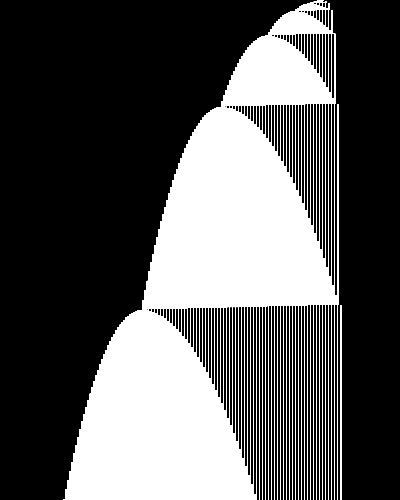
\includegraphics[width=0.7\linewidth]{figures/space-time-diagrams/bb5_20k.png} % Adjust the path as needed
        \caption{20,000-step \textit{zoomed out} space-time diagram of the 5-state winner.}\label{fig:bb5-diagram-zoomout}
    \end{subfigure}
    \hfill
    \begin{subfigure}[t]{0.45\textwidth}
        \centering
        \vspace{10pt} % Adjust vertical alignment
        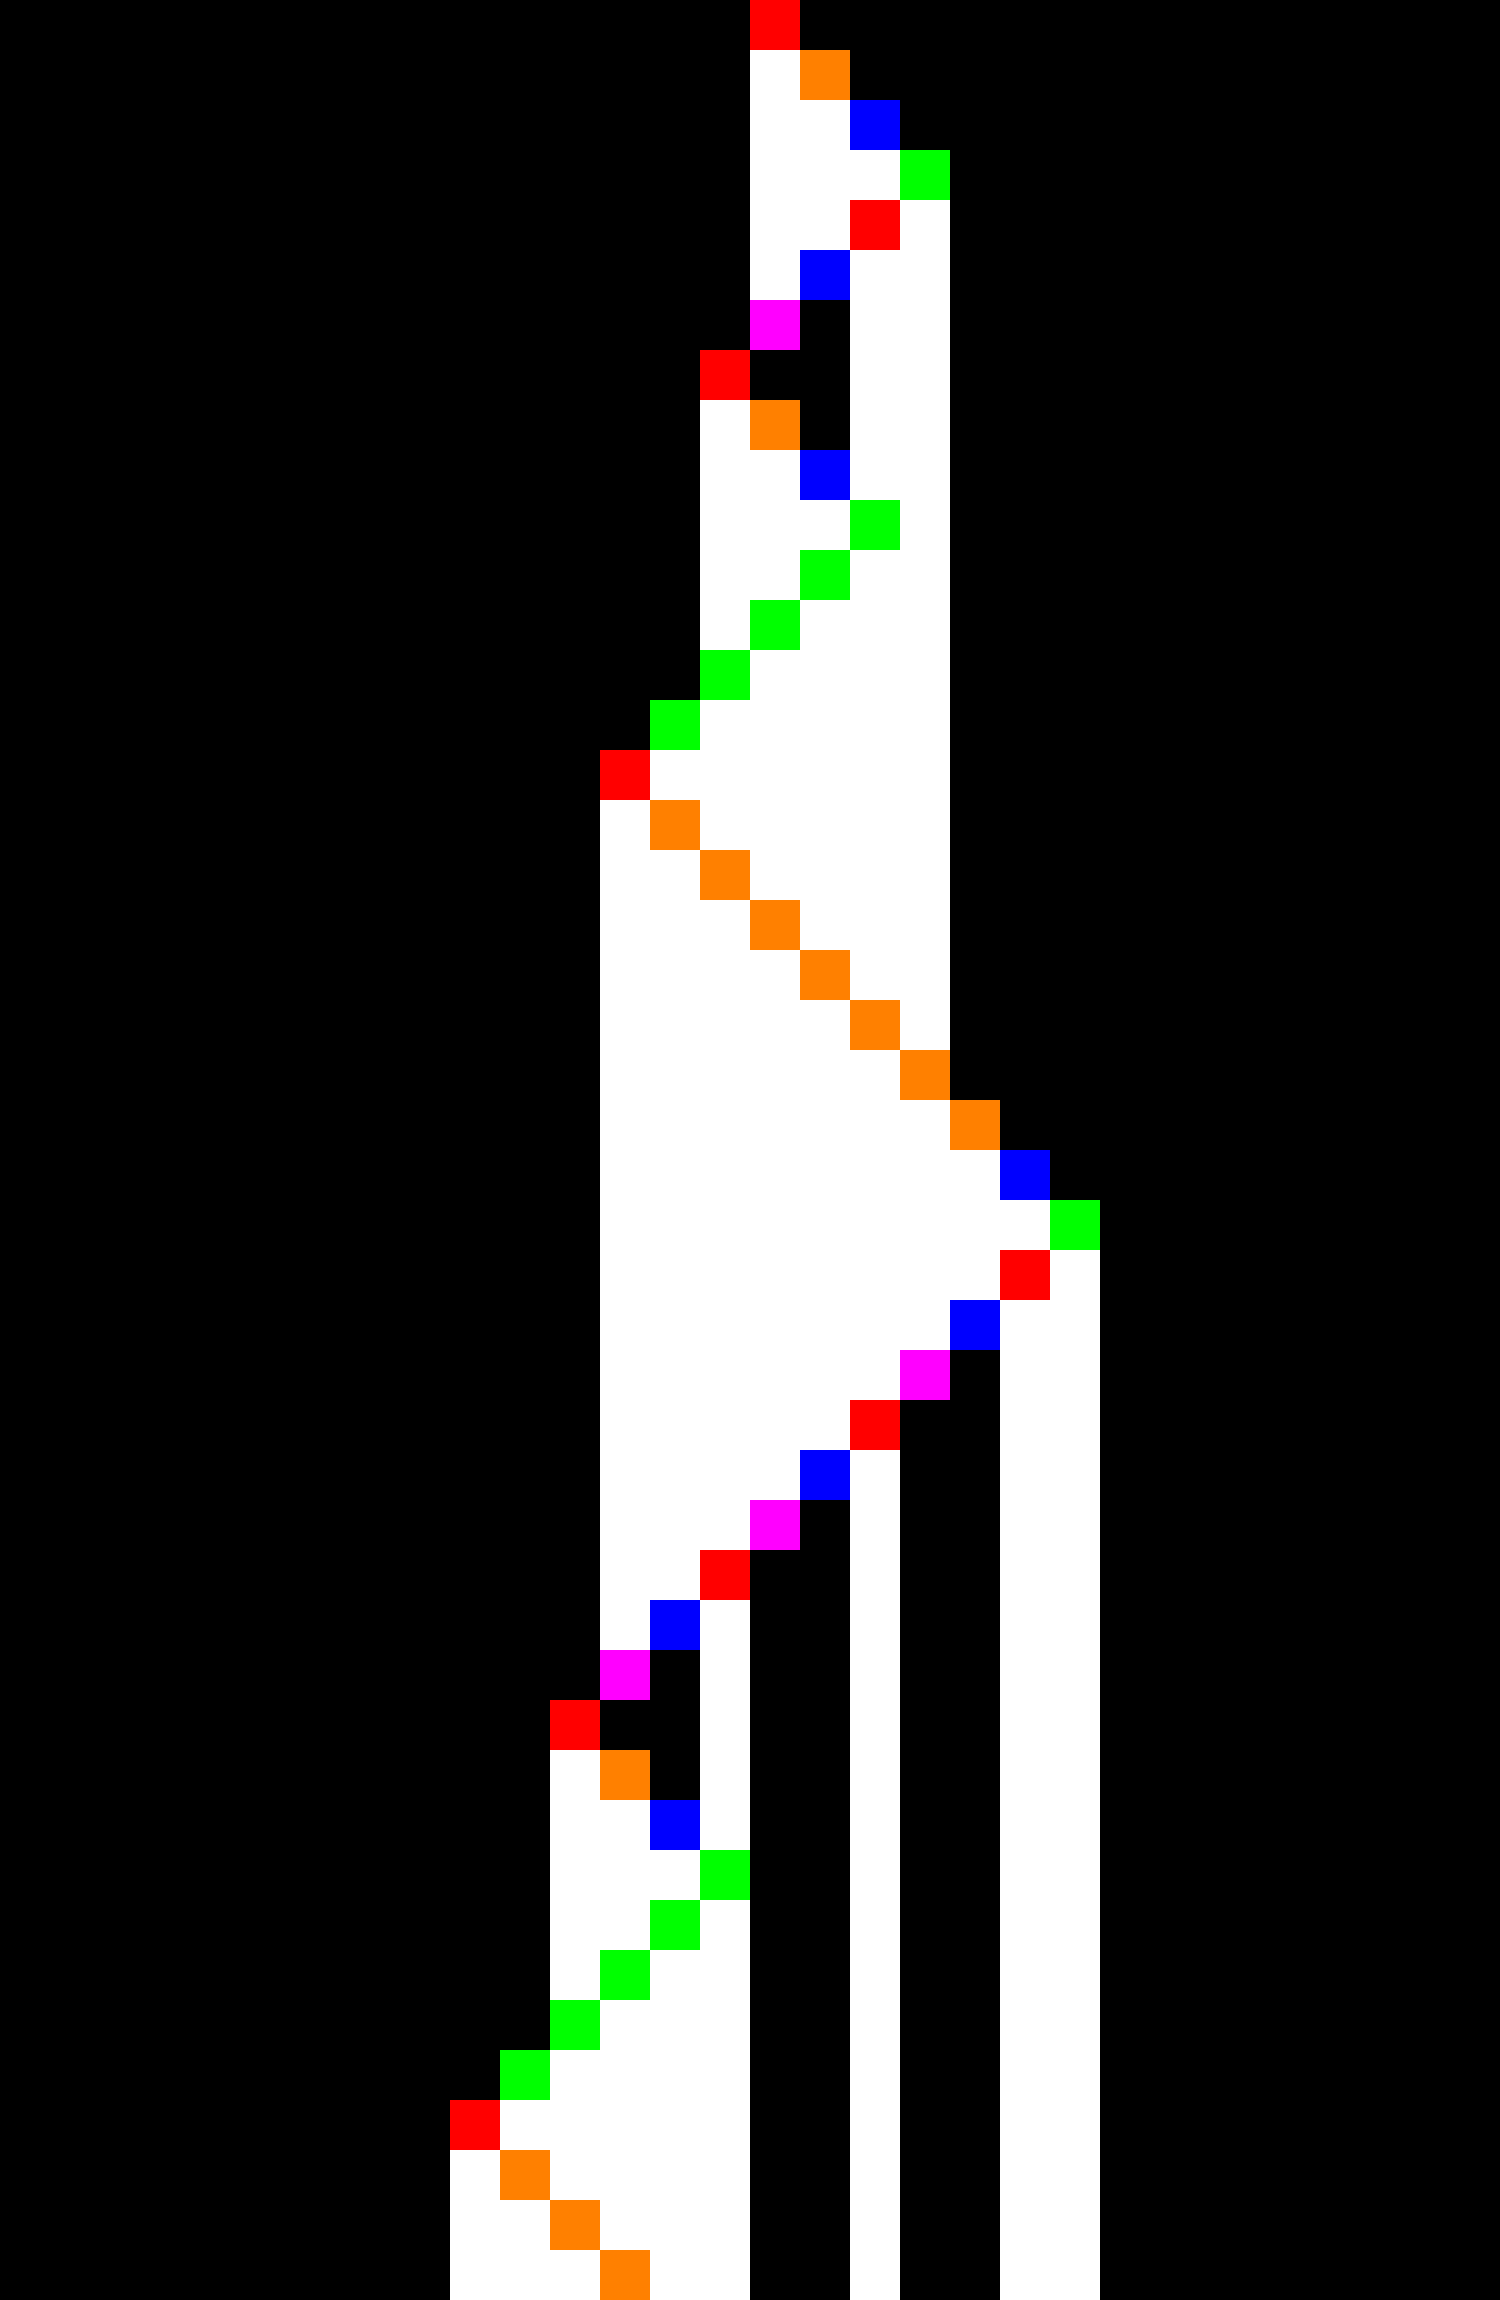
\includegraphics[width=0.7\linewidth]{figures/space-time-diagrams/bb5.pdf}
        \caption{Space-time diagram of the first 45 steps of the 5-state winner.}
        \label{fig:bb5-diagram}
    \end{subfigure}
    \caption{Transition table and space-time diagrams of the 5-state 2-symbol busy beaver winner, which halts after 47,176,870 steps.
        \url{https://bbchallenge.org/1RB1LC_1RC1RB_1RD0LE_1LA1LD_---0LA}.}
    \label{fig:bb5}
\end{figure}


We consider Turing machines that use a single, discrete, bi-infinite tape -- \ie the tape can be thought of a function $t: \mathbb{Z} \to \alphabet$ with $\alphabet$ the alphabet of symbols used by the machine. Machine transitions are either undefined (the machine halts if it ever reaches an undefined transition) or given by (a) a symbol of $\alphabet$ to write (b) a direction to move (right or left) and (c) a state to go to -- \ie the transition table of a Turing machine is a partially defined function $\delta: \text{States} \times \alphabet \to \alphabet \times \{\text{L},\text{R}\} \times \text{States}$. Figure~(\ref{table:bb5}) gives the transition table of the 5-state 2-symbol \BBfull winner. The machine halts after 47,176,870 steps (starting from all-0 tape) when it reads a \szero in state \stateE (undefined transition).

In the \BBfull context, machines are always executed from the all-0 tape and starting in state \stateA. Execution goes as follows: at each step, the machine which is in state $s$ looks at which symbol $\sigma$ is present on the tape cell the head is currently on and then, if defined, executes the instruction given by its transition table, \eg $\delta(s, \sigma) = 0\text{L}\text{\stateE}$ means that the machine will write a \szero, move the cell on the left of the current one and switch to state \stateE. If $\delta(s, \sigma)$ is not defined, the machine halts.



A \textit{configuration} (also known as \textit{execution state}) of a Turing machine is defined by the 3-tuple: (i) state (ii) position of the head on the tape (iii) content of the memory tape. As mentioned above, here, \textit{the initial configuration} of a machine is always (i) state is A, i.e. the first state to appear in the machine's description (ii) head's position is 0 (iii) the initial tape is all-0 -- i.e. each memory cell is containing 0. We write $c_1 \TMstep_\mathcal{M} c_2$ if a configuration $c_2$ is obtained from $c_1$ in one computation step of machine $\mathcal{M}$. We omit $\mathcal{M}$ if it is clear from context. We let $c_1 \TMstep^s c_2$ denote a sequence of $s$ computation steps, and let $c_1 \TMstep^* c_2$ denote zero or more computation steps. % exact same wording as in https://dna.hamilton.ie/assets/dw/NearyWoodsFCT09.pdf
We write $c_1 \TMstep \bot$ if the machine halts after executing one computation step from configuration $c_1$. Halting happens when an undefined machine transition is met i.e. no instruction is given for when the machine is in the state, tape position and tape corresponding to configuration $c_1$.

% When discussing concrete configurations, we write
% $0^\infty\; s_1\; \cdots\; s_{k-1}\; [s_k]_q\; s_{k+1}\; \cdots\; s_n\; 0^\infty$
% to mean the configuration where the machine is in state $q$, with the head
% positioned on the symbol $s_k$, and the tape both starts and end by an infinite sequence of 0s, represented $0^\infty$. Thus, the initial configuration of the machine
% can be written as $0^\infty\; [0]_A\; 0^\infty$.

% \paragraph*{Directional Turing machines.} We will sometimes prefer to think of the tape head as being between
% symbols. Thus, we write $l \lhead{q} r$, with $l,r\in\{0,1\}^*$ to mean that the head is at the rightmost symbol
% of $l$, and $l \rhead{q} r$ to mean that the head is at the leftmost symbol of $r$.
% For example, $0^\infty\; [1]_A\; 0^\infty$ can be written as
% $0^\infty\; 1 \lhead A 0^\infty$ or $0^\infty \rhead A 1\; 0^\infty$.


\paragraph*{Space-time diagrams.} We use space-time diagrams to give a visual representation of the behavior of a given machine. The space-time diagram of machine $\mathcal{M}$ is an image where the $i^\text{th}$ row of the image gives:
\begin{enumerate}
    \item The content of the tape after $i$ steps (for 2-symbol machines, black is 0 and white is 1, while for $n$ symbols, black is 0, white is symbol $n-1$ and linear gray-scaling is used in between).
    \item The position of the head is colored to give state information using the following colours for 5-state machines: \textcolor{colorA}{A},  \textcolor{colorB}{B},  \textcolor{colorC}{C},  \textcolor{colorD}{D},  \textcolor{colorE}{E} (you have to look at the row above to deduce what symbol is the head reading, unless it is the initial row, where a \szero is read).
\end{enumerate}

Figure~(\ref{fig:bb5-diagram}) gives a 45-step space-time diagram for the 5-state 2-symbol \BBfull winner. We often use \textit{zoomed-out} space-time diagrams without state-coloring information, such as Figure~(\ref{fig:bb5-diagram-zoomout}) which gives the 20,000 first steps of the 5-state 2-symbol \BBfull winner.


\paragraph*{Turing machine format.} We often communicate Turing machines using the following linear format: \\ \texttt{1RB1LC\_1RC1RB\_1RD0LE\_1LA1LD\_---0LA} represents the transition table of Figure~\ref{table:bb5} where \texttt{\_} is used to separate states and transitions are given in read-symbol order. Note that, historically, the undefined transition reached by a halting machine was represented using \texttt{1RZ}, hence our format allows to use any letter outside of the state space to represent halting, \eg \texttt{1RB1LC\_1RC1RB\_1RD0LE\_1LA1LD\_1RZ0LA}. Multi-symbols machines are represented in the same way, \eg the 2-state 4-symbol \BBfull winner is \texttt{1RB2LA1RA1RA\_1LB1LA3RB---} (also given by \texttt{1RB2LA1RA1RA\_1LB1LA3RB1RZ}), see Figure~\ref{fig:bb2x4}.

This format can be used as URL for the \url{bbchallenge.org} website, \eg \url{https://bbchallenge.org/1RB1LC\_1RC1RB\_1RD0LE\_1LA1LD\_1RZ0LA} will display the transition table, space-time diagrams and known information about the machine.

\begin{figure}[h!]
    \centering
    \begin{subfigure}[t]{0.45\textwidth}
        \centering
        \renewcommand{\arraystretch}{1.3} % Increase row height
        \setlength{\tabcolsep}{12pt} % Increase column spacing
        \vspace{10pt} % Adjust vertical alignment
        \begin{tabular}{cccccc}
            \toprule
                    & \textbf{0} & \textbf{1} & \textbf{2} & \textbf{3} \\
            \midrule
            \stateA & 1R\stateB  & 2L\stateA  & 1R\stateA  & 1R\stateA  \\
            \stateB & 1L\stateB  & 1L\stateA  & 3R\stateB  & ---        \\
            \bottomrule
        \end{tabular}
        \caption{Transition table of the 2-state 4-symbol \BBfull winner.}
        \label{table:bb2x4}

        \vspace{10pt} % Adjust spacing
        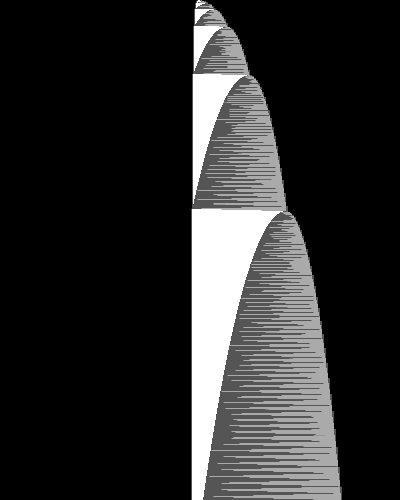
\includegraphics[width=0.7\linewidth]{figures/space-time-diagrams/bb2x4_20k.png} % Adjust the path as needed
        \caption{20,000-step \textit{zoomed out} space-time diagram of the 2-state 4-symbol winner.}\label{fig:bb2x4-diagram-zoomout}
    \end{subfigure}
    \hfill
    \begin{subfigure}[t]{0.45\textwidth}
        \centering
        \vspace{10pt} % Adjust vertical alignment
        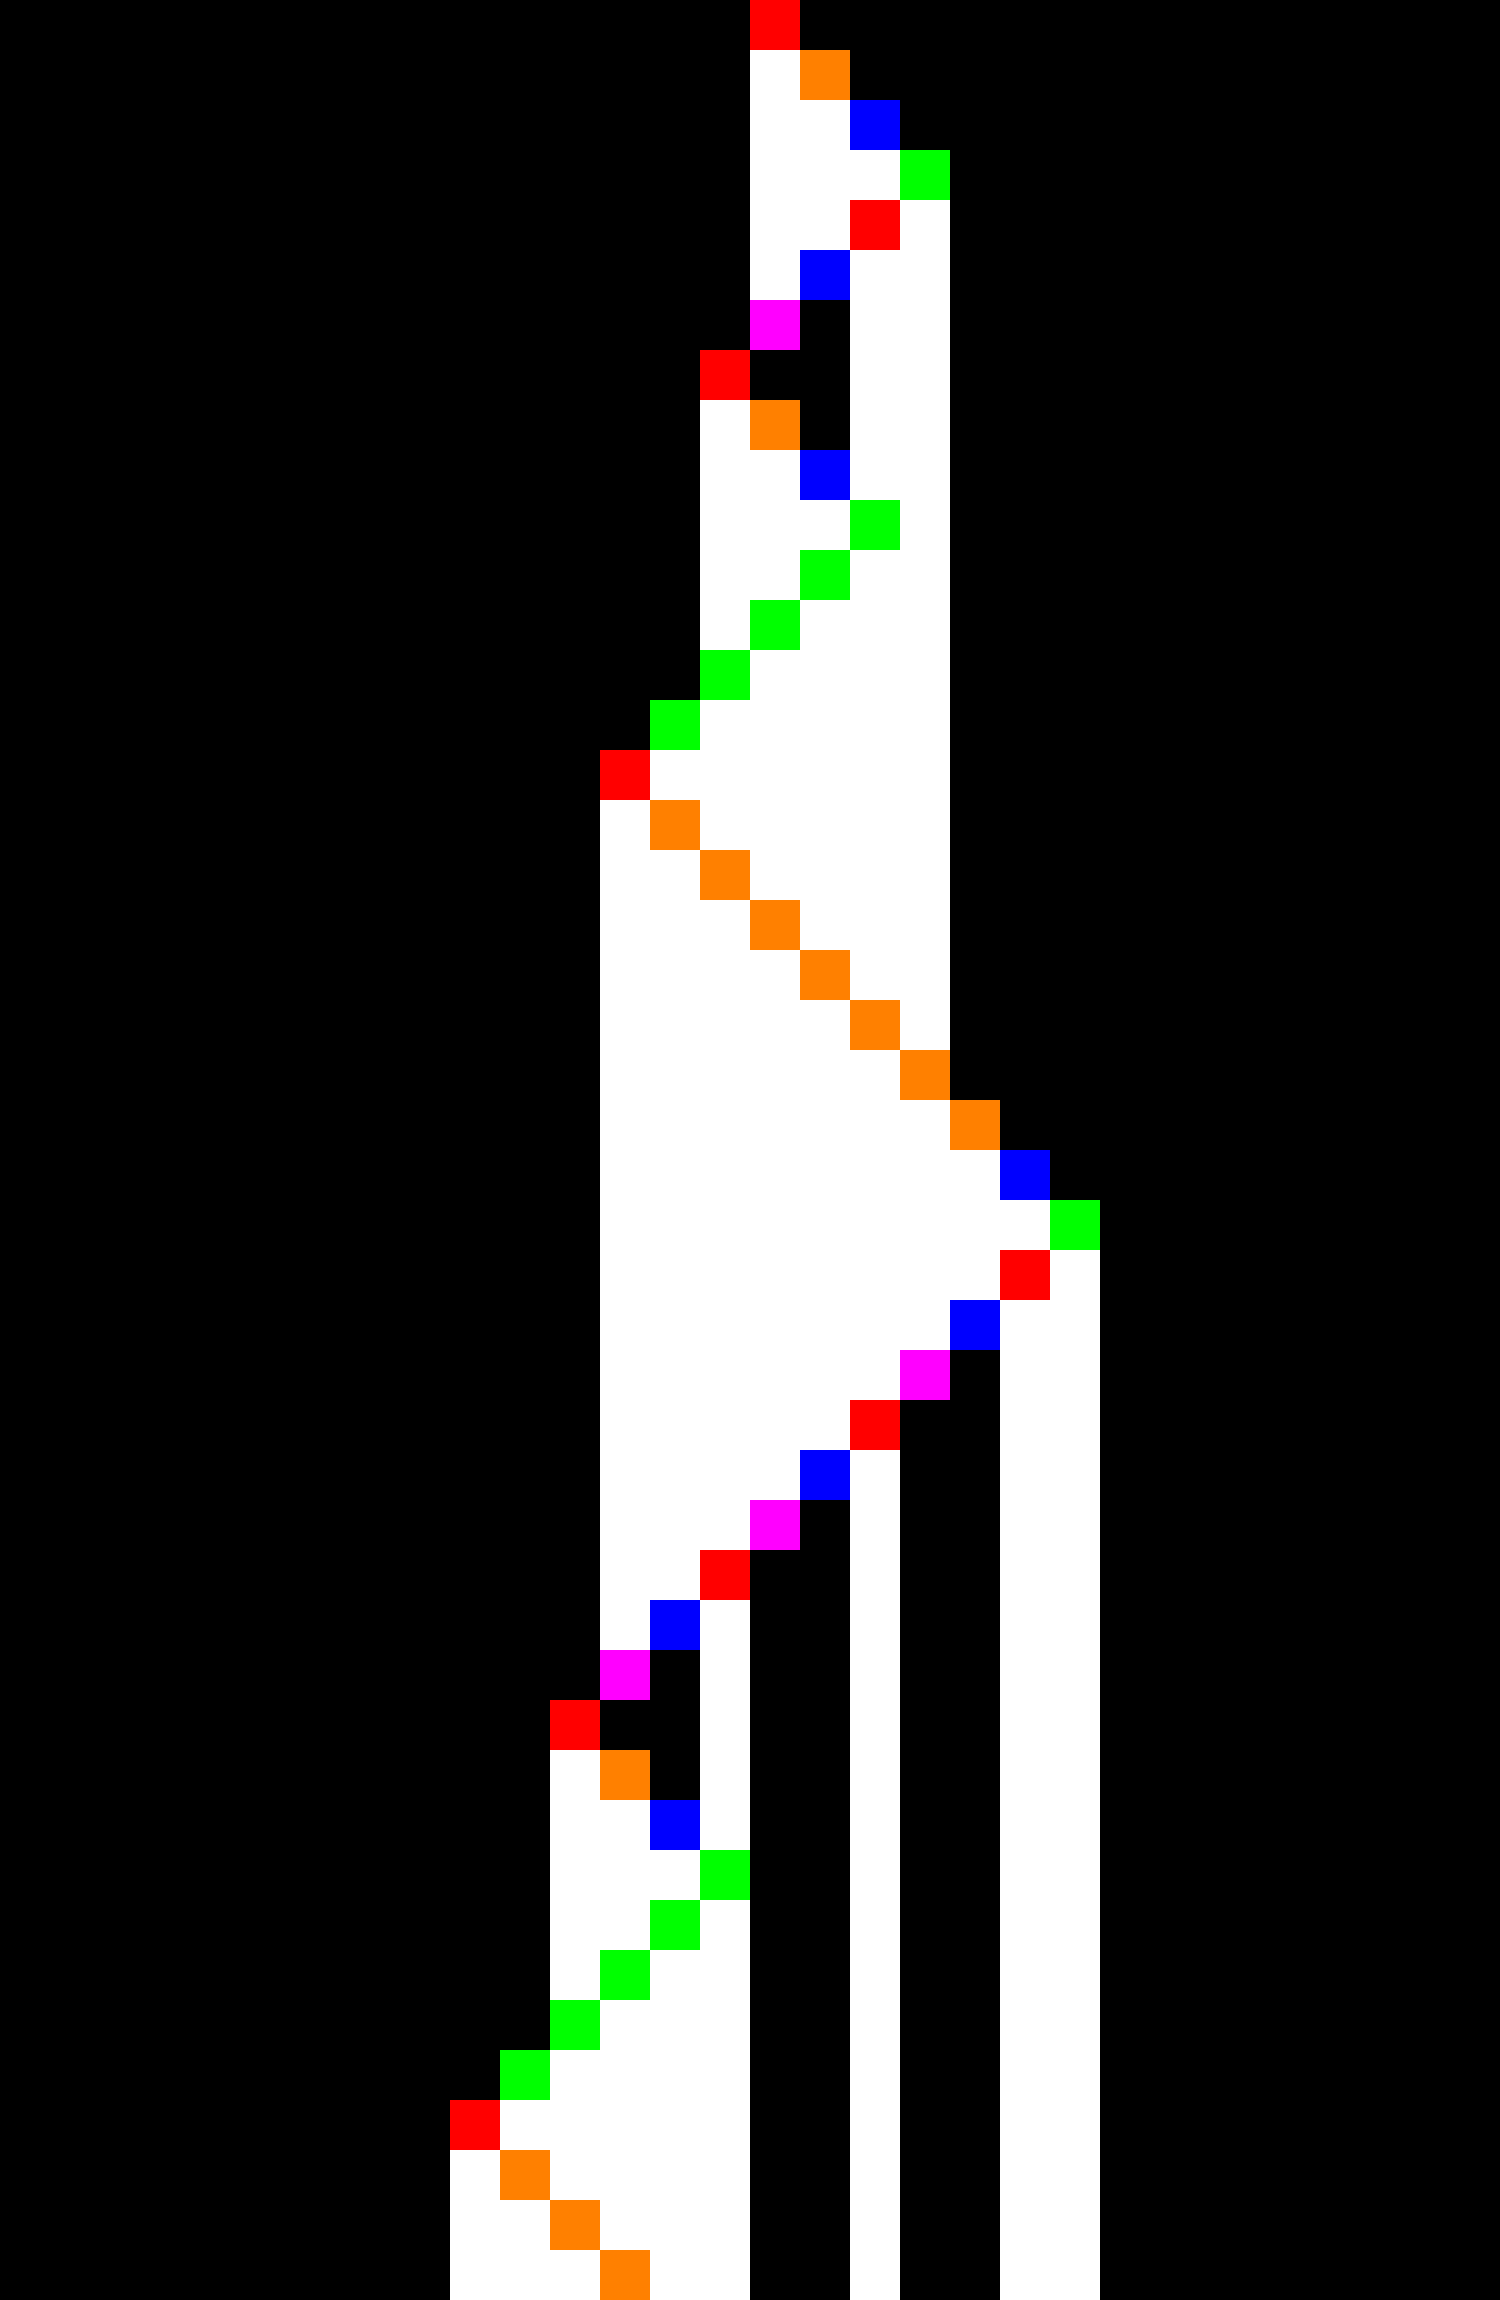
\includegraphics[width=0.7\linewidth]{figures/space-time-diagrams/bb5.pdf}
        \caption{Space-time diagram of the first 45 steps of the 2-state 4-symbol winner.}
        \label{fig:bb2x4-diagram}
    \end{subfigure}
    \caption{Transition table and space-time diagrams of the 2-state 4-symbol \BBfull winner, which halts after $\BBTxF$ steps.
        \url{https://bbchallenge.org/https://bbchallenge.org/1RB2LA1RA1RA_1LB1LA3RB---}.}
    \label{fig:bb2x4}
\end{figure}

\newpage
\section{Tree Normal Form machine enumeration (TNF)}\label{sec:enum}

\newpage
\section{Deciders}\label{sec:deciders}

A \textit{decider} is a program that takes as input a Turing machine $\mathcal{M}$ and that returns either \HALT, \NONHALT, \UNKNOWN whether it was able to detect that the machine's halting status (halt or nonhalt) or not.

\subsection{Pipelines}\label{sec:pipelines}
A \textit{pipeline} of deciders consists of applying several deciders in sequence: a machine is tested by each decider successively until one decider outputs \HALT or \NONHALT. Table~\ref{tab:pipelineBB5} gives an approximation of the pipeline of deciders implemented in \CoqBB in order to decide all the $\BBtheFifthTNF$ enumerated 5-state machines (see Section~\ref{sec:enum}) and that way, conclude that $S(5) = \BBtheFifth$ since any machine running more steps is decided \NONHALT, see Theorem~\ref{th:BB5}. Similarly, Table~\ref{tab:pipelineBB2x4} and Table~\ref{tab:pipelineBB4} repsectively approximations of the pipelines leading to $S(2,4) = \BBTxF$ and $S(4) = \BBtheFourth$ -- the latter confirming the result for $S(4)$ given in \cite{Brady83}.

The exact pipelines are give in Appendix~\ref{app:pipelines} and only differ in that the precise parameters and sometimes algorithmic variants are given for each decider which are sometimes interleaved with each other (\eg the decider for loops is first called with a small step-count parameter, then other deciders are applied and later on it is called again with higher step-count parameter).

\ts{TS: I'm hesitating to say this early that a subtlelty of the S(5) pipeline is that parameters (or, more "concerning" certificates) are given hardocded for approx 8k machines. Also questionning to say (or repeat) here that WFAR is irregular (as well as some sporadic), which makes a disctinction between S(5) and S(4)/S(2,4).}

\begin{table}[h!]

    \begin{tabular}{llll}
        $S(5)$ decider pipeline                                                              & Nonhalt                         & Halt                           & Total decided \\
        \hline
        1. Loops, see \textbf{Section~\ref{sec:loops}}                                       & 126,994,099                     & 48,379,711                     & 175,373,810   \\
        2. $n$-gram Closed Position Set (NGramCPS), see \textbf{Section~\ref{sec:n-gramCPS}} & 6,005,142                       & 0                              & 6,005,142     \\
        3. Repeated Word List (RepWL), see \textbf{Section~\ref{sec:RepWL}}                  & 6,577                           & 0                              & 6,577         \\
        4. Finite Automata Reduction (FAR), see \textbf{Section~\ref{sec:FAR}}               & 32                              & 0                              & 32            \\
        5. Weighted Finite Automata Reduction (WFAR), see \textbf{Section~\ref{sec:WFAR}}    & 31                              & 0                              & 31            \\
        6. Long halters (simulation up to $\BBtheFifth$ steps)                               & 0                               & 183                            & 183           \\
        7. Sporadic machines, individual proofs, see \textbf{Section~\ref{sec:sporadic}}     & 14                              & 0                              & 14            \\ \hline
        Total                                                                                & \multicolumn{1}{r}{133,005,895} & \multicolumn{1}{r}{48,379,894} & 181,385,789
    \end{tabular}
    \caption{Approximation of the $S(5)$ decider pipeline as implemented in \CoqBB. All the $\BBtheFifthTNF$ enumerated 5-state machines are decided by this pipeline, which solves $S(5) = \BBtheFifth$, see Theorem~\ref{th:BB5}. The exact pipeline, with deciders parameters is given in Appendix~\ref{app:pipelines}. }\label{tab:pipelineBB5}
\end{table}

\begin{table}[h!]

    \begin{tabular}{llll}
        $S(2,4)$ decider pipeline                                                            & Nonhalt & Halt & Total decided \\
        \hline
        1. Loops, see \textbf{Section~\ref{sec:loops}}                                       &         &      &               \\
        2. $n$-gram Closed Position Set (NGramCPS), see \textbf{Section~\ref{sec:n-gramCPS}} &         &      &               \\
        3. Repeated Word List (RepWL), see \textbf{Section~\ref{sec:RepWL}}                  &         &      &               \\
        4. Long halters (simulation up to $\BBTxF$ steps)                                    &         &      &               \\
        \\ \hline
        Total                                                                                &         &      &
    \end{tabular}
    \caption{Approximation of the $S(2,4)$ decider pipeline as implemented in \CoqBB. All the $\BBTxFTNF$ enumerated 2-state 4-symbol machines are decided by this pipeline, which solves $S(2,4) = \BBTxF$, see Theorem~\ref{th:BB2x4}. The exact pipeline, with deciders parameters is given in Appendix~\ref{app:pipelines}. }\label{tab:pipelineBB2x4}
\end{table}

\begin{table}[h!]

    \begin{tabular}{llll}
        $S(4)$ decider pipeline                                                              & Nonhalt & Halt & Total decided \\
        \hline
        1. Loops, see \textbf{Section~\ref{sec:loops}}                                       &         &      &               \\
        2. $n$-gram Closed Position Set (NGramCPS), see \textbf{Section~\ref{sec:n-gramCPS}} &         &      &               \\
        3. Repeated Word List (RepWL), see \textbf{Section~\ref{sec:RepWL}}                  &         &      &               \\
        \\ \hline
        Total                                                                                &         &      &
    \end{tabular}
    \caption{Approximation of the $S(4)$ decider pipeline as implemented in \CoqBB. All the $\BBtheFourthTNF$ enumerated 4-state machines are decided by this pipeline, which brings confirmation that $S(4) = \BBtheFourth$ \cite{Brady83}, see Theorem~\ref{th:BB4}. The exact pipeline, with deciders parameters is given in Appendix~\ref{app:pipelines}. }\label{tab:pipelineBB4}
\end{table}



% !TeX root = ../bbchallenge-paper.tex

\newpage
\subsection{Loops}\label{sec:loops}

\begin{figure}[h!]
  \centering
  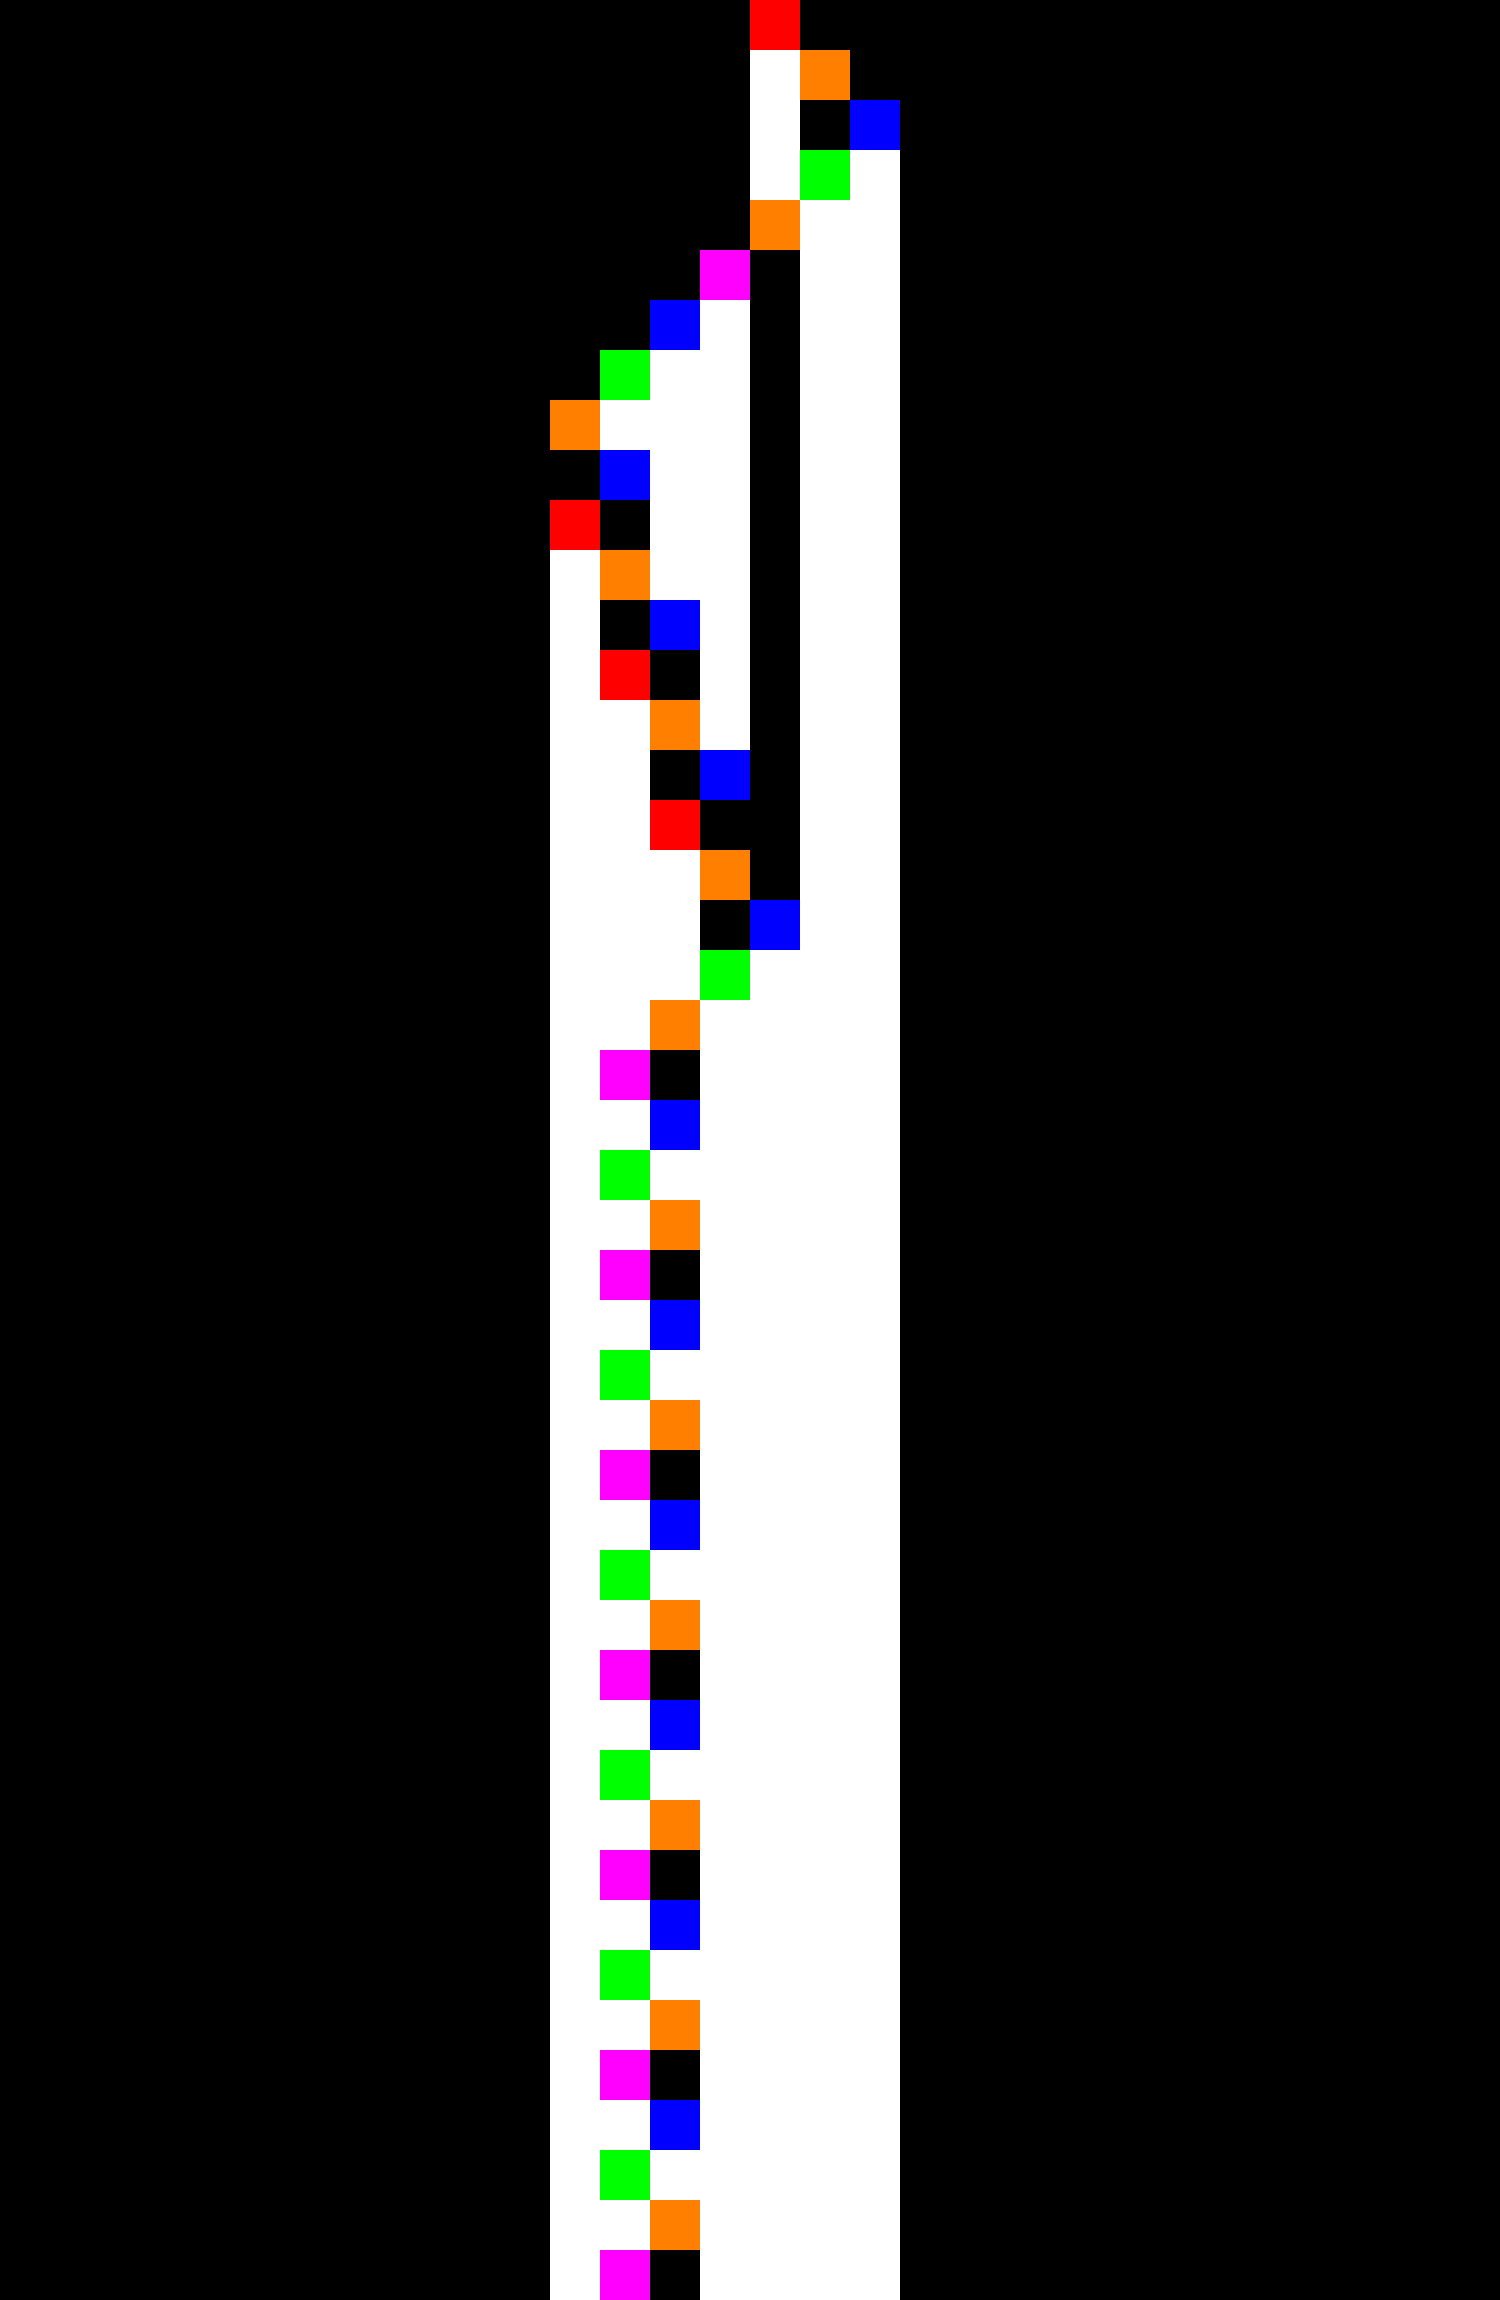
\includegraphics[width=0.4\textwidth]{figures/space-time-diagrams/cycler_279081.pdf}
  \hspace{2ex}
  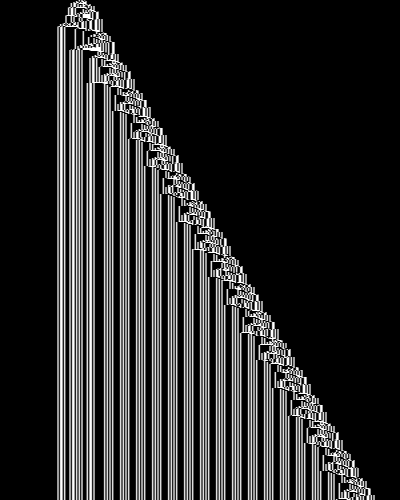
\includegraphics[width=0.4\textwidth]{figures/space-time-diagrams/translated_cycler_59090563_2.png}
  \caption{Space-time diagrams of the 30 first steps of a \textit{\cycler} with colors indicating head position and state (left) and of the 10,000 first steps of a \TC (right). \cyclers are machines that eventually repeat the same configuration forever. \TCs are machines that eventually repeats the same configuration forever, but translated in space. We refer to these two types of machines as \textit{loops}.}\label{fig:loops}
\end{figure}

The goal of this decider is to recognise \textit{Loops} which are Turing machines that eventually repeat the same configuration forever (called \textit{\cyclers}, Figure~\ref{fig:loops}~left), potentially translated in space (called \textit{\TCs}, Figure~\ref{fig:loops}~right).

Deciding Cyclers reduces to the well-known mathematical problem of detecting the cycles of a function for which standard algorithms exist \cite{wiki:Cycle_detection}, the simplest one consisting in memorizing each successive configuration of the machine until encountering one that has been already seen. Translated Cyclers, also known as \textit{Lin's recurrence}, have first been described and decided in Shen Lin's 1963 PhD thesis \cite{Lin1963}, other algorithms to detect them have been developed since then\footnote{\url{https://discuss.bbchallenge.org/t/decider-translated-cyclers/34}}.

Here, we develop a new algorithm (Algorithm~\ref{alg:loops}) for deciding both \cyclers and \TCs. The particularity of this algorithm is that it detects cyclers only by analysing the history of \ssps seen by the machine's head instead of considering entire configurations (\ie with full tape content information). This algorithm is also able to detect if a machine halts and in practice detects 99.99\% of all enumerated halting machines \ts{TS: link to section/table about stats or something and maybe link to the pipeline figure}.

\newpage
\begin{algorithm}
  \caption{{\sc decider-Loops}}\label{alg:loops}

  \begin{algorithmic}[1]
    \State{\textbf{Input:} A Turing machine `$\mathcal{M}$', a step limit parameter $L$.}
    \State{\textbf{Output:} `NON-HALT' if the decider detects that the machine is a loop, `HALT' if the machine halts and `UNKNOWN' otherwise.}

    \State
    \State Simulate $\mathcal{M}$ for $L$ steps and save the history of
    each consecutive state, read-symbol and tape position reached, \ie consecutive $h_i = (s_i,m_i,d_i) \in \states \times \alphabet \times \Z$ for $0 \leq i \leq L$ and $h_0 = (\stateA,\symbolzero,0)$.


    \State \If{the machine has halted before $L$ steps}
    \State \Return HALT
    \EndIf
    \State \For{$l$ \textbf{in} $[0,+\infty[$ } \Comment{$l+1$ is the length of the potential loop}
    \State \If{$2(l + 1) > L$} \Comment{The history does not contain two potential loops of size $l+1$}
    \State \Return UNKNOWN
    \State \EndIf
    \State $K = L-l-1$
    \State $\text{allseen} = \text{true}$
    \State $\text{recordbreak} = \text{false}$
    \State \For{$i$ \textbf{in} $[0,l]$ } \Comment{Comparing \ssp equality at each step of both potential loops}
    \State $s,m,d = h_{L-i}$
    \State $s',m',d' = h_{K-i}$ \Comment{$d'$ will not be used}
    \State \If{$s\neq s'$ \textbf{or} $m \neq m'$}
    \State $\text{allseen} = \text{false}$
    \State \textbf{break}
    \EndIf
    \State \If{$d > \text{max} \{d_j \, | \, j < L-i \}$ \textbf{or} $d < \text{min} \{d_j \, | \, j < L-i \}$}
    \State $\text{recordbreak} = \text{true}$
    \EndIf
    \EndFor
    \State \If{$\text{allseen}$ \textbf{and} ($d_L == d_K$ \textbf{or} $\text{recordbreak}$)}
    \State \Return NON-HALT
    \EndIf
    \EndFor


  \end{algorithmic}
\end{algorithm}
% \input{sections/decider-1-translated-cyclers.tex}
% !TeX root = ../bbchallenge-paper.tex

\newpage
\subsection{n-gram Closed Position Set (NGramCPS)}\label{sec:n-gramCPS}

\newcommand{\alphabet}{\mathcal{A}}
\newcommand{\leftngram}{left\xspace}
\newcommand{\rightngram}{right\xspace}
\newcommand{\middlesymbol}{middle\xspace}

\begin{algorithm}
    \caption{{\sc decider-NGramCPS}}\label{alg:NGramCPS}

    \begin{algorithmic}[1]
        \State{\textbf{Input:} a Turing machine `tm', the zero symbol of the alphabet $\alphabet_0$, the size of the n-grams $r > 0$.}
        \State{\textbf{Output:} `NON-HALT' if the decider detects that the machine doesn't halt and `UNKNOWN' otherwise.}

        \State $g_0 = (\alphabet_0)^r$ \Comment{The zero n-gram consists of $r$ zero symbols}
        \State $L = \{ g_0 \}$ \Comment{The seen left n-grams}
        \State $R = \{ g_0 \}$ \Comment{The seen right n-grams}
        \State $C =$ \{\{.\leftngram $=$ $g_0$, .\rightngram $=$ $g_0$, .\middlesymbol $=$ $\alphabet_0$, .state $=$ \textcolor{colorA}{A} \}\} \Comment{The seen local contexts}
        \While{true}
        \State $V = C$
        \State any\_updates $=$ false
        \While{$|V| \neq 0$}
        \State $c = V.\textbf{pop}()$
        \State $c' = c$
        \State $\{w,d,s\}$ $=$ tm(c.state, c.\middlesymbol) \Comment{Transition's write symbol, move direction, and next state}
        \State \If{$s$ is undefined} \Comment{Undefined transition is met}
        \State \textbf{return} UNKNOWN
        \EndIf
        \State \If{$d$ is Right}
        \State Add $c.\text{\leftngram}$ to $L$ \Comment{$c.\text{\leftngram}$ is the falling n-gram}
        \State Set $c'.\text{\leftngram}$ to the last $r-1$ symbols of $c.\text{\leftngram}$ followed by $w$
        \State Set $c'.\text{\middlesymbol}$ to the first symbol of $c.\text{\rightngram}$
        \For{each ngram $r\in R$ starting with the last $r-1$ symbols of $c.\text{\rightngram}$}
        \State Set $c'.\text{\rightngram}$ to $r$
        \If{$c'$ is not in $C$}
        \State \tabi Insert $c'$ in $C$
        \State \tabi Insert $c'$ in $V$
        \State \tabi any\_updates $=$ true
        \EndIf
        \EndFor
        \EndIf
        \State \If{$d$ is Left}
        \State Add $c.\text{\rightngram}$ to $R$ \Comment{$c.\text{\rightngram}$ is the falling n-gram}
        \State Set $c'.\text{\rightngram}$ to the first $r-1$ symbols of $c.\text{\rightngram}$ preceded by $w$
        \State Set $c'.\text{\middlesymbol}$ to the last symbol of $c.\text{\leftngram}$
        \For{each ngram $l \in L$ ending with the first $r-1$ symbols of $c.\text{\leftngram}$}
        \State Set $c'.\text{\leftngram}$ to $l$
        \If{$c'$ is not in $C$}
        \State \tabi Insert $c'$ in $C$
        \State \tabi Insert $c'$ in $V$
        \State \tabi any\_updates $=$ true
        \EndIf
        \EndFor
        \EndIf
        \EndWhile
        \State \If{\textbf{not} any\_updates}
        \State \textbf{return} NON-HALT
        \EndIf

        \EndWhile
    \end{algorithmic}
\end{algorithm}
\newpage
% !TeX root = ../bbchallenge-paper.tex

\newpage
\subsection{Repeated Word List (RepWL)}\label{sec:RepWL}

The Repeated Word List (RepWL) technique is based on the following simple idea: if a word (or \textit{block}) of length $l > 0$ appears consecutively on the tape more than $T > 0$ times (with $T, l \in \mathbb{N}$ fixed) then, let's assume it will eventually repeat forever. In practice, it means we represent configurations as regular expressions. For instance, consider the following configuration:

$$ \texttt{0}^\infty \; \texttt{1100 A> 111101010101000000} \; \texttt{0}^\infty$$

Using $l=2$ and $T = 3$, we represent it as (treating $\texttt{0}^\infty$ as implicit border condition):

$$ (\texttt{11})^2 \; (\texttt{00}) \; \texttt{A>} \; (\texttt{11})^2 \; (\texttt{01})^{3+} \; (\texttt{00})^{3+}$$

Where regular expression $(w)^{k+}$ means that the word $w$ is repeated at least $k$ times, with $w \in \{\szero,\sone\}^*$ and $k > 0$. Note that here, we use \textit{directional head notation} for Turing machines, where the head lives in between cells and points either right or left. This framework is equivalent to the Turing machines setup (Appendix~\ref{app:TMs}) used elsewhere in this work.

We now need to deal with two cases: (i) \textit{block simulation} when the head is facing a constant block (\ie block without a $+$), such as $\texttt{A>} \; (\texttt{11})^2$ and (ii) \textit{regex branching} when the head is facing a block with a $+$, \eg $\texttt{B>} \; (\texttt{01})^3+$.

\paragraph{Block simulation.} When the head is facing a constant block, such as in the above example $\texttt{A>} \; (\texttt{11})^2$, we can proceed to \textit{block simulation}. Block simulation consists in simulating the Turing machine until the head potentially eventually leaves the block. We say potentially as the machine could enter a cycle inside the block and never leave it. In practice this is dealt with either using a gas parameter limiting how many steps we're willing to take in block simulation before giving up (option taken in \CoqBB), or to embed a decider for loops in the block simulator (Section~\ref{sec:loops}). For instance, block simulation from $\texttt{A>} \; (\texttt{11})^2$ could produce, for instance, $(\texttt{00})^2 \; \texttt{B>}$ or $\texttt{<C} \; \texttt{10} \; \texttt{11} $ or enter a cycle and never leave the block.

\paragraph{Regex branching.} When the head is facing a block with a $+$, for instance $\texttt{B>} \; (\texttt{01})^{3+}$, we add two configurations to the set of configurations to visit next:
\begin{enumerate}
    \item A configuration where $\texttt{B>} \; (\texttt{01})^{3+}$ is replaced with $\texttt{B>} \; (\texttt{01}) \; (\texttt{01})^{2}$
    \item A configuration where $\texttt{B>} \; (\texttt{01})^{3+}$ is replaced with  $\texttt{B>} \; (\texttt{01}) \; (\texttt{01})^{3+}$
\end{enumerate}
In both case, we've reduced to block simulation.

\paragraph{RepWL decider.} Starting from the initial configuration (\ie $\texttt{A>}$, assuming that $0^\infty$ are treated as implicit border conditions), using block simulation and regex branching, we're creating a graph of regex configurations to explore -- nodes using regex branching have out-degree two. If this graph is eventually closed and contains no halting configuration then we know that the machine will never halt (Theorem~\ref{th:repwl}) since we have constructed a set of configurations bigger than the one it will visit and that does not contain any halting transition.
% !TeX root = ../bbchallenge-paper.tex

\newpage
\subsection{Finite automata reduction (FAR)}\label{sec:FAR}

% \paragraph{Acknowledgement.} Sincere thanks to bbchallenge's contributor Justin Blanchard who initially presented this method and the first implementation\footnote{See: \url{https://discuss.bbchallenge.org/t/decider-finite-automata-reduction/}.}. Others have contributed to this method by producing alternative implementations (see Section~\ref{sec:far-implem}) or discussing and writing the formal proof presented here: Tony Guilfoyle, Tristan Stérin (cosmo), Nathan Fenner, Mateusz Naściszewski (Mateon1), Konrad Deka, Iijil, Shawn Ligocki. %, savask.


% \subsubsection{Method overview}\label{far-overview}

% The core idea of Finite Automate Reduction (FAR) is to find, for a given Turing machine, a regular language that contains the set of the machine's eventually-halting configurations (with finitely many 1s). Then, provided that the all-0 configuration is not in the regular language, we know that the machine does not halt.

% In this section, we limit ourselves to Turing machines configurations with finite support, \ie configurations with finitely many \texttt{1}s (or, more generally, finitely many non-\texttt{0} symbols) and, when we write \textit{configuration}, we mean, \textit{configuration with finite support}.

\subsubsection{Overview}

\newcommand{\M}{M}
\newcommand{\T}{^{T}}

Finite Automata Reduction (FAR) is a \textit{co-CTL} technique, \ie it is dual to the Closed Tape Language (CTL) framework given in Section~\ref{sec:deciders-overview}: for a given Turing machine, we are looking for a regular language that contains the set of the machine's eventually-halting configurations and, provided that the all-0 configuration is not in the regular language, we know that the machine does not halt.

The specificity of FAR is to restrict regular languages to a class of Nondeterministic Finite Automata (NFA) -- those satisfying Theorem~\ref{far-main-theorem} -- for which it is computationally simple to verify that they have the co-CTL properties: (i) reject the all-0 initial configuration, (ii) closed under Turing machines transitions, (iii) accept all eventually-halting configurations.

In \CoqBB, FAR is only used as a \textbf{verifier} meaning that specific Turing machines together with their FAR NFAs are directly hardcoded in the proof (in file \texttt{Verifier\_FAR\_Hardcoded\_Certificates.v}) and then verified using Theorem~\ref{far-main-theorem} -- see Section~\ref{sec:FAR:results} for results. FAR was originally developed by Blanchard as a fully-fledged decider -- \ie the verifier together with search algorithms for NFAs \cite{FAR}.

We only present the verifier part of FAR, which is encompassed in Theorem~\ref{far-main-theorem}.

\subsubsection{Verifier theorem}

In the following, we limit ourselves to Turing machines configurations with finite support, \ie configurations with finitely many \texttt{1}s (or, more generally, finitely many non-\texttt{0} symbols) and, when we write \textit{configuration}, we mean, \textit{configuration with finite support}.

A Turing machine configuration $c$ is represented as a finite word, called a \textit{word-representation} of $c$, by concatenating the tape content (from left to right, making sure to include all the \texttt{1}s) and adding the state (in our case, a letter from A to E) just before the position of the head. For instance, two word-representations of the configuration on the top row of Figure~\ref{fig:finite-automata-reduction}(c), are $\hat{c} = \texttt{00A001100}$ and $\hat{c}' = \texttt{000A00110000}$. Word-representations of the same configuration will only differ in the number of leading and trailing \texttt{0}s that they have.


Then, a co-CTL regular language of word-represented configurations $\mathcal{L}$ for a Turing machine $\mathcal{M}$ satisfies:
\begin{align}
    u \in \mathcal{L}                               & \iff 0u \in \mathcal{L}           &  & \text{(leading zeros ignored)}
    \label{eq:lzignore}
    \\
    u \in \mathcal{L}                               & \iff u0 \in \mathcal{L}           &  & \text{(trailing zeros ignored)}
    \label{eq:tzignore}
    \\
    c\TMstep\bot                                    & \implies \hat{c} \in \mathcal{L}  &  & \text{(recognising halt, base case)} \nonumber \\
    (c_1\TMstep c_2)\land \hat{c}_2 \in \mathcal{L} & \implies\hat{c}_1 \in \mathcal{L} &  & \text{(recognising halt, induction)} \nonumber
\end{align}


With $c, c_1, c_2$ configurations of $\mathcal{M}$ (with finite support) and $\hat{c}, \hat{c}_1, \hat{c}_2$ any of their word-representations.


Given how word-representations are defined, the last two above conditions become:
\begin{align}
    \forall u,z\in\{0, 1\}^*: \; ufrz \in \mathcal{L},\;                                                           & \text{if $\delta(f,r)$ is undefined (\ie halting)} \label{eq:h0}
    \\
    \forall u,z\in\{0, 1\}^*,\,\forall b \in \{0, 1\}: utbwz \in \mathcal{L} \implies ubfrz \in \mathcal{L},\;     & \text{if $\delta(f,r) = (w,\text{L},t)$} \label{eq:hnl}
    \\
    \forall u,z\in\{0, 1\}^*,\,\forall b \in \{0, 1\}: u w t z \in \mathcal{L} \implies u f r z \in \mathcal{L},\; & \text{if $\delta(f,r) = (w,\text{R},t)$} \label{eq:hnr}
\end{align}

With $f,t \in \{\stateA,\stateB,\stateC,\stateD,\stateE\}$ the ``from'' and ``to'' states in a transition, $r,w,b \in \{0,1\}$ the bit ``read'', the bit ``written'', and just a bit, and $\delta$ the transition table (see Section~\ref{sec:TMs}) of $\mathcal{M}$.

%\footnote{A semiring is a ring without the requirement to have additive inverses, e.g. the set of natural numbers $\N=\{0,1,2\dots\}$ is a semiring.}

We now transform Conditions~\eqref{eq:lzignore}–\eqref{eq:hnr} into, sometimes stronger, conditions on the structure of NFAs -- using the usual linear-algebraic description of NFAs, which we first recall. Let $\mathbf{2}$ denote the Boolean semiring $\{0,1\}$ with operations $+$ and $\cdot$ respectively implemented by $\operatorname{OR}$ and $\operatorname{AND}$ \cite{CUNINGHAMEGREEN1991251}. Let $\M_{m,n}$ be the set of matrices with $m$ rows and $n$ columns over $\mathbf{2}$. We may define a Nondeterministic Finite Automaton (NFA) with $n$ states and alphabet $\mathcal{A}$ as a tuple $(q_0, \{T_\gamma\}_{\gamma \in \mathcal{A}}, a)$ where $q_0 \in \M_{1,n}$ and $a \in \M_{1,n}$ respectively represent the initial states and accepting states of the NFA. (i.e. if the $i^\text{th}$ state of the NFA is an initial state then the $i^\text{th}$ entry of $q_0$ is set to 1 and the rest are 0, and the $i^\text{th}$ entry of $a$ is set to 1 if and only if the $i^\text{th}$ state of the NFA is accepting), and where transitions are matrices $T_\gamma\in \M_{n,n}$ for each $\gamma\in\mathcal{A}$ (i.e. the entry $(i,j)$ of matrix $T_\gamma$ is set to 1 iff the NFA transitions from state $i$ to state $j$ when reading $\gamma$). Furthermore, for any word $u=\gamma_1\dots\gamma_\ell \in \mathcal{A}^*$, let $T_u = T_{\gamma_1} T_{\gamma_2} \dots T_{\gamma_\ell}$ be the state transformation resulting from reading word $u$ (Note: $T_\epsilon = I$). A word $u=\gamma_1\dots\gamma_\ell \in \mathcal{A}^*$ is accepted by the NFA iff there exists a path from an initial state to an accepting state that is labelled by the symbols of $u$, which algebraically translates to $q_0 T_u a\T = 1$ with $a\T \in \M_{n,1}$ the transposition of $a$.

Using this algebraic framework, Conditions~\eqref{eq:lzignore}~and~\eqref{eq:tzignore} are implied by the following stronger conditions on transition matrix $T_0 \in \M_{n,n}$:
\begin{align}
    q_0 T_0 & = q_0
    \label{far-cond-leading-0}
    \\
    T_0 a\T & = a\T
    \label{far-cond-trailing-0}
\end{align}

Indeed, Condition~\eqref{far-cond-leading-0} transparently ignores leading zeros, Condition~\eqref{far-cond-trailing-0} means that for all accepting states of the NFA, reading a \szero is possible and leads to an accepting state since $T_0 a\T$ describes the set of NFA states that reach the set of accepting states $a$ after reading a \szero.

Then, Conditions~\ref{eq:h0}--\eqref{eq:hnr} algebraically translate to:
{\small
\begin{align*}
    \forall u,z\in\{0, 1\}^*: \; q_0 T_u T_f T_r T_z a\T = 1, \;                                                                           & \text{if $\delta(f,r)$ is undefined (\ie halting)}
    \\
    \forall u,z\in\{0, 1\}^*,\,\forall b \in \{0, 1\}: q_0 T_{u} T_t T_b T_w T_{z} a\T = 1 \implies q_0 T_{u} T_b T_f T_r T_{z} a\T = 1,\; & \text{if $\delta(f,r) = (w,\text{L},t)$}
    \\
    \forall u,z\in\{0, 1\}^*,\,\forall b \in \{0, 1\}: q_0 T_{u} T_w T_t T_{z} a\T = 1 \implies q_0 T_{u} T_f T_r T_{z} a\T = 1,\;         & \text{if $\delta(f,r) = (w,\text{R},t)$}
\end{align*}
}

These conditions are unwiedly. We seek stronger (thus still sufficient) conditions which are simpler:

\begin{itemize}

    \item For machine transitions going left/right, simply require $T_t T_b T_w\preceq T_b T_f T_r$ and $T_w T_t\preceq T_f T_r$, respectively with $\preceq$ the following relation on same-size matrices: $M\preceq M'$ if $M_{ij}\le M'_{ij}$ element-wise, that is, if the second matrix has at least the same 1-entries as the first matrix.

    \item To simplify the condition for halting machine transitions: define an \emph{accepted steady state-set} $s$ to be a row vector such that $sa\T = 1$, $s T_0\succeq s$, and $s T_1\succeq s$. Given such $s$, we have that: $\forall q\in\M_{1,n}\; q \succeq s\implies \forall z\in\{0, 1\}^*: qT_{z}a\T = 1$. Assuming that such $s$ exists we can simply require: $\forall u\in\{0, 1\}^*: q_0T_u T_f T_r \succeq s$ which is stronger than $\forall u,z\in\{0, 1\}^*: \; q_0 T_u T_f T_r T_z a\T = 1$ with $(f,r) \to \bot$ a halting transition.

          % \footnote{\ts{Note that our new condition $\forall u\in\{0, 1\}^*: q_0T_u T_f T_r \succeq s$ requires that $\forall u\in\{0, 1\}^*: q_0T_u \neq 0$, i.e. that reading 0 and 1 from the initial states must always lead to some state. This assertion is not limiting since if it is not met by some NFA, adding an additional sink state to the NFA will not change the recognised language and will satisfy the assertion.}}

          % assert that for all $u \in \{0, 1\}^*$, the sub-expression $q_0 T_{u}$ is not zero \ts{(this means that reading 0 and 1 from the initial states must always lead to some state\footnote{This assertion is not limiting since if it is not met by some NFA, adding an additional sink state to the NFA will not change the recognised language and will satisfy the assertion.})},
          % and \tss{(for $q$ a nonzero combination of such vectors and $fr\TMstep\bot$ a halt rule)}{that $q_0 T_{u} T_f T_r$}
          % is a vector $q'$ satisfying $\forall z\in\{0, 1\}^*: q' T_{z} a = 1$ \ts{(this means that the NFA will accept any word containing a halting transition independently of the bits written after the machine's head)}.

          % Given such $s$, we have $q'\succeq s\implies \forall z\in\{0, 1\}^*: q'T_{z}a = 1$.
\end{itemize}

Combining the above, we get FAR:



\begin{theorem}[\CoqBB: \texttt{Lemma dfa\_nfa\_verifier\_spec}\footnote{\CoqBB's lemma is slightly different, as it builds the NFA satisfying this theorem using a given ``precursor'' Deterministic Finite Automaton (DFA) -- as initially developed in \cite{FAR} -- see Section~\ref{sec:FAR:results}.}]
    \label{far-main-theorem}
    Machine $\mathcal{M}$, with transition table $\delta$ (see Section~\ref{sec:TMs}), doesn't halt from the initial all-0 configuration if there is a Nondeterministic Finite Automaton $(q_0, \{T_\gamma\}, a)$ and row vector $s$ satisfying the below:
    \begin{align}
        \label{far-cond-first}
        q_0 T_0                                & = q_0
                                               &                     & \text{(leading zeros ignored)}
        \tag{\ref{far-cond-leading-0}}
        \\
        T_0a\T                                 & = a\T
                                               &                     & \text{(trailing zeros ignored)}
        \tag{\ref{far-cond-trailing-0}}
        \\
        sa\T                                   & = 1
                                               &                     & \text{($s$ is accepted)}
        \label{far-cond-ass-accepted}
        \\
        sT_0,sT_1                              & \succeq s
                                               &                     & \text{($s$ is a steady state)}
        \label{far-cond-ass-steady}
        \\
        \forall u\in\{0, 1\}^*: q_0T_u T_f T_r & \succeq s
                                               &                     & \text{if $\delta(f,r)$ is undefined (\ie halting)}
        \label{far-cond-halt}
        \\
        \forall b\in\{0, 1\}: T_b T_f T_r      & \succeq T_t T_b T_w
                                               &                     & \text{if $\delta(f,r) = (w,\text{L},t)$}
        \label{far-cond-left}
        \\
        T_f T_r                                & \succeq T_w T_t
                                               &                     & \text{if $\delta(f,r) = (w,\text{R},t)$}
        %\label{far-cond-right}
        \label{far-cond-last}
        \\
        q_0 T_A a\T                            & = 0
                                               &                     & \text{(initial configuration rejected)}
        \label{far-cond-reject-start}
    \end{align}
\end{theorem}
\begin{proof}
    Conditions \eqref{far-cond-leading-0}--\eqref{far-cond-last} ensure that the NFA's language includes at least all eventually halting configurations of $\mathcal{M}$, see above. Condition~\eqref{far-cond-reject-start} ensures that the initial all-0 configuration of the machine is rejected, hence not eventually halting. Hence, if conditions \eqref{far-cond-leading-0}--\eqref{far-cond-reject-start} are satisfied, we can conclude that $\mathcal{M}$ does not halt from the initial all-0 configuration.
\end{proof}

\paragraph{Verifier.} Theorem~\ref{far-main-theorem} has the nice property of being easy to verify: given a Turing machine, an NFA and a vector $s$, the task of verifying that equations \eqref{far-cond-first}--\eqref{far-cond-reject-start} hold and thus that the machine does not halt, is computationally simple\footnote{Note that although equation~\eqref{far-cond-halt} has a $\forall u\in\{0, 1\}^*$ quantification, the set of NFA states reachable after reading an arbitrary $u \in \{0,1\}^*$ is computable, and we just have to consider one instance of equation~\eqref{far-cond-halt} replacing $q_0 T_u$ per such state.}.



\subsubsection{Implementations and results}\label{sec:FAR:results}



% The regular languages considered by FAR are described using Nondeterministic Finite Automata (NFA) and one important aspect of the technique is that, given a Turing machine and its FAR NFA, it is a computationally simple task to verify that the NFA's language does indeed recognise at least all the eventually-halting configurations of the machine.

% Concretely, a Turing machine configuration $c$ is represented as a finite word, called a \textit{word-representation} of $c$, by concatenating the tape content (from left to right, making sure to include all the \texttt{1}s) and adding the state (in our case, a letter from A to E) just before the position of the head. For instance, two word-representations of the configuration on the top row of Figure~\ref{fig:finite-automata-reduction}(c), are $\hat{c} = \texttt{00A001100}$ and $\hat{c}' = \texttt{000A00110000}$. Word-representations of the same configuration will only differ in the number of leading and trailing \texttt{0}s that they have.

% Then, given this encoding of configurations, for a given Turing machine $\mathcal{M}$, by definition, a co-CTL regular language $\mathcal{L}$ satisfies:
% \begin{align}
%     u \in \mathcal{L} \iff 0u \in \mathcal{L}                                         &  & \text{(leading zeros ignored)}
%     \label{eq:lzignore}
%     \\
%     u \in \mathcal{L} \iff u0 \in \mathcal{L}                                         &  & \text{(trailing zeros ignored)}
%     \label{eq:tzignore}
%     \\
%     c\TMstep\bot  \implies \hat{c} \in \mathcal{L}                                    &  & \text{(recognising halt, base case)}\label{eq:h0} \\
%     (c_1\TMstep c_2)\land \hat{c}_2 \in \mathcal{L} \implies\hat{c}_1 \in \mathcal{L} &  & \text{(recognising halt, induction)}\label{eq:hn}
% \end{align}


% With $c, c_1, c_2$ configurations of $\mathcal{M}$ (with finite support) and $\hat{c}, \hat{c}_1, \hat{c}_2$ any of their word-representations. \\



% FAR represents regular languages using Nondeterministic Finite Automata (NFA) and makes use of their algebraic presentation: let $\mathbf{2}$ denote the Boolean semiring\footnote{A semiring is a ring without the requirement to have additive inverses, e.g. the set of natural numbers $\N=\{0,1,2\dots\}$ is a semiring.} $\{0,1\}$ with operations $+$ and $\cdot$ respectively implemented by $\operatorname{OR}$ and $\operatorname{AND}$ \cite{CUNINGHAMEGREEN1991251}. Let $\M_{m,n}$ be the set of matrices with $m$ rows and $n$ columns over $\mathbf{2}$. We may define a Nondeterministic Finite Automaton (NFA) with $n$ states and alphabet $\mathcal{A}$ as a tuple $(q_0, \{T_\gamma\}_{\gamma \in \mathcal{A}}, a)$ where $q_0 \in \M_{1,n}$ and $a \in \M_{1,n}$ respectively represent the initial states and accepting states of the NFA. (i.e. if the $i^\text{th}$ state of the NFA is an initial state then the $i^\text{th}$ entry of $q_0$ is set to 1 and the rest are 0, and the $i^\text{th}$ entry of $a$ is set to 1 if and only if the $i^\text{th}$ state of the NFA is accepting), and where transitions are matrices $T_\gamma\in \M_{n,n}$ for each $\gamma\in\mathcal{A}$ (i.e. the entry $(i,j)$ of matrix $T_\gamma$ is set to 1 iff the NFA transitions from state $i$ to state $j$ when reading $\gamma$). Furthermore, for any word $u=\gamma_1\dots\gamma_\ell \in \mathcal{A}^*$, let $T_u = T_{\gamma_1} T_{\gamma_2} \dots T_{\gamma_\ell}$ be the state transformation resulting from reading word $u$ (Note: $T_\epsilon = I$). A word $u=\gamma_1\dots\gamma_\ell \in \mathcal{A}^*$ is accepted by the NFA iff there exists a path from an initial state to an accepting state that is labelled by the symbols of $u$, which algebraically translates to $q_0 T_u a\T = 1$ with $a\T \in \M_{n,1}$ the transposition of $a$.

% Using this algebraic framework, Equations~\eqref{eq:lzignore}~and~\eqref{eq:tzignore} are implied by the following stronger conditions on transition matrix $T_0 \in \M_{n,n}$:
% \begin{align}
%     q_0 T_0 & = q_0
%     \label{far-cond-leading-0}
%     \\
%     T_0 a\T & = a\T
%     \label{far-cond-trailing-0}
% \end{align}

% Indeed, Equation~\eqref{far-cond-leading-0} means that reading a \szero in the initial state $q_0$ leads back to $q_0$, while Equation~\eqref{far-cond-trailing-0}, means that for all accepting states of the NFA, reading a \szero is possible and leads to an accepting state since $T_0 a\T$ describes the set of NFA states that reach the set of accepting states $a$ after reading a $0$.



% A dual idea has been explored by other authors under the name Closed Tape Languages (CTL) as described in S. Ligocki's blog \cite{ShawnCTL} and credited to H. Marxen in collaboration with J. Buntrock.
% The CTL technique for proving a Turing machine doesn't halt is to exhibit a set $C$ of configurations such that:

% \begin{enumerate}
%     \item $C$ contains the all-0 initial configuration\footnote{
%               Criteria 1--2 give a strict definition; in \cite{ShawnCTL}, $C$ only needs to contain some descendant of the initial configuration and some descendant of the successor to each $c\in C$.
%               In that case, the set of ancestor configurations to those in $C$ meets the strict definition.
%           }
%     \item $C$ is \textit{closed} under transitions: for any $c \in C$, the configuration one step later belongs to $C$\addtocounter{footnote}{-1}\addtocounter{Hfootnote}{-1}\footnotemark
%     \item $C$ does not contain any halting configuration
% \end{enumerate}


% If such a set $C$ exists then the machine does not halt.
% The CTL approach has proven to be practical and powerful when we search for $C$ among regular languages \cite{ShawnCTL} \cite{BruteforceCTL}.

% Here, we develop an original \textit{co-CTL} technique\footnote{By co-CTL we mean a set whose complement is a CTL, characterized by closure criteria inverse---or equivalently converse---to 1--3. In other words, a co-CTL contains all halting configurations, any configuration which can \emph{precede} any member configuration by one TM transition, and not the initial configuration.}, based on the algebraic description of Nondeterministic Finite Automata (NFA), for finding a regular language which contains a machine's eventually halting configurations (in general a superset).

% One important aspect of the technique is that, given a Turing machine and its constructed NFA---if found---it is a computationally simple task to verify that the NFA's language does indeed recognise all eventually-halting configurations (with finitely many 1s) of the machine.


% \usetikzlibrary {automata, positioning}

% \begin{figure}
%     \begin{center}
%         \begin{tikzpicture}[scale=0.2]
%             \tikzstyle{every node}+=[inner sep=0pt]
%             \draw [black] (32.4,-20.7) circle (3);
%             \draw (32.4,-20.7) node {$X$};
%             \draw [black] (19.9,-32.9) circle (3);
%             \draw (19.9,-32.9) node {$Y$};
%             \draw [black] (43.9,-32.9) circle (3);
%             \draw (43.9,-32.9) node {$Z$};
%             \draw [black] (43.9,-32.9) circle (2.4);
%             \draw [black] (12.2,-32.9) -- (16.9,-32.9);
%             \fill [black] (16.9,-32.9) -- (16.1,-32.4) -- (16.1,-33.4);
%             \draw [black] (32.4,-13.6) -- (32.4,-17.7);
%             \fill [black] (32.4,-17.7) -- (32.9,-16.9) -- (31.9,-16.9);
%             \draw [black] (31.917,-23.654) arc (-16.01031:-75.38142:12.771);
%             \fill [black] (31.92,-23.65) -- (31.22,-24.28) -- (32.18,-24.56);
%             \draw (29.58,-29.75) node [below] {$\alpha$};
%             \draw [black] (20.894,-35.718) arc (47.15723:-240.84277:2.25);
%             \draw (18.84,-40.19) node [below] {$\alpha$};
%             \fill [black] (18.27,-35.4) -- (17.36,-35.65) -- (18.09,-36.33);
%             \draw [black] (20.283,-29.932) arc (165.64786:102.96041:12.277);
%             \fill [black] (29.42,-21.01) -- (28.53,-20.7) -- (28.76,-21.68);
%             \draw (22.58,-23.71) node [above] {$\beta$};
%             \draw [black] (34.46,-22.88) -- (41.84,-30.72);
%             \fill [black] (41.84,-30.72) -- (41.66,-29.79) -- (40.93,-30.48);
%             \draw (37.62,-28.27) node [left] {$\beta$};
%             \draw [black] (34.454,-18.529) arc (164.32314:-123.67686:2.25);
%             \draw (39.49,-17.55) node [right] {$\beta$};
%             \fill [black] (35.37,-21.01) -- (36.01,-21.71) -- (36.28,-20.74);
%             \draw [black] (45.807,-35.201) arc (67.3925:-220.6075:2.25);
%             \draw (46.66,-40.1) node [below] {$\alpha,\beta$};
%             \fill [black] (43.23,-35.81) -- (42.47,-36.36) -- (43.39,-36.74);
%             \draw [black] (41.27,-34.338) arc (-65.18014:-114.81986:22.321);
%             \fill [black] (22.53,-34.34) -- (23.05,-35.13) -- (23.47,-34.22);
%             \draw (31.9,-36.9) node [below] {$\alpha$};
%         \end{tikzpicture}
%     \end{center}
%     \caption{Example Nondeterministic Finite Automaton (NFA) with 3 states X, Y and Z, alphabet $\mathcal{A} = \{\alpha,\beta\}$, initial states X and Y, and accepting state Z. The linear-algebra representation of this NFA is given in Example~\ref{ex:nfa}. Example accepted words are: $\beta$, $\alpha\beta$, $\alpha\alpha\beta\beta$. Example rejected words are: $\alpha$, $\alpha\alpha$, $\alpha\alpha\alpha$.}\label{fig:example_nfa}
% \end{figure}

% \begin{figure}

%     % \begin{subfigure}[m]{0.13\textwidth}
%     %   \centering
%     %   \includegraphics[width=\textwidth]{figures/space-time-diagrams/finite-automata-reduction-counter4.pdf}
%     %   \caption{First few descendants of \tss{a 4-state TM's}{the initial all-0 configuration for the machine given in (\ref{fig:far_transitions})}.}
%     %   \label{fig:far_spacetime}
%     % \end{subfigure}
%     % \hfill
%     % \parbox{0.2\textwidth}{
%     %   \begin{subfigure}[t]{0.22\textwidth}
%     %     \centering
%     %     \includegraphics[width=\textwidth]{figures/space-time-diagrams/finite-automata-reduction-counter4-halt.pdf}
%     %     \caption{\tss{The same TM halts in these configurations.}{Some  eventually-halting successive configurations of the machine given in (\ref{fig:far_transitions}): the machine halts after 18 steps by reading a 0 in state D.}}
%     %     \label{fig:far_spacetime_halt}
%     %   \end{subfigure}
%     %   \vspace{0.23\textheight}

%     %   \begin{subfigure}[t]{0.2\textwidth}
%     %     \centering
%     %     \begin{tabular}{lll}
%     %                             & 0                       & 1                       \\
%     %       \textcolor{colorA}{A} & 1R\textcolor{colorB}{B} & 0L\textcolor{colorD}{D} \\
%     %       \textcolor{colorB}{B} & 1L\textcolor{colorC}{C} & 1R\textcolor{colorA}{A} \\
%     %       \textcolor{colorC}{C} & 0R\textcolor{colorB}{B} & 0L\textcolor{colorC}{C} \\
%     %       \textcolor{colorD}{D} & - - -                   & 1L\textcolor{colorA}{A} \\
%     %     \end{tabular}
%     %     \caption{Transition table.}
%     %     \label{fig:far_transitions}
%     %   \end{subfigure}
%     % }
%     % \hfill
%     % \begin{subfigure}[m]{0.62\textwidth}
%     %   \begin{tikzpicture}[shorten >=1pt]
%     %     \node[state,initial above] (0) at (-2, 2) {0};
%     %     \node[state]           (1) at (-2, -2) {1};
%     %     \node[state,accepting] (H) at (2, 4) {$\bot$};
%     %     \node[state]           (0A) at (0, 2) {0A};
%     %     \node[state,accepting] (0D) at (4, 2) {0D};
%     %     \node[state]           (0B) at (2, 0) {0B};
%     %     \node[state]           (0C) at (4, 0) {0C};
%     %     \node[state]           (1C) at (2, -2.5) {1C};
%     %     \node[state]           (1B) at (0, -4) {1B};
%     %     \node[state]           (1A) at (4, -4) {1A};
%     %     \node[state,accepting] (1D) at (5.5, -2) {1D};

%     %     \path[->]  (0)  edge [loop right]       node {$0$} (0)
%     %     edge                    node [right] {$1$} (1)
%     %     (1)  edge [bend left=15]     node [above left] {$0|1$} (0)
%     %     (0A) edge                    node [right] {$0$} (1B)
%     %     edge                    node [above,rotate=60] {$1$} (H)
%     %     (0C) edge                    node [above] {$0$} (0B)
%     %     edge                    node [right] {$1$} (1A)
%     %     (0D) edge                    node [above,rotate=300] {$0$} (H)
%     %     edge                    node [above] {$1$} (0A)
%     %     edge [bend left]        node [left] {$1$} (1A)
%     %     (1A) edge                    node [above] {$1$} (1B)
%     %     (1A) edge [bend right=15]    node [above,rotate=300] {$0|1$} (0B)
%     %     (0B) edge [bend right=5]     node [above,rotate=300] {$0|1$} (1A)
%     %     (1B) edge                    node [above right,rotate=60] {$0$} (0B)
%     %     edge [loop left]        node {$0$} (1B)
%     %     edge [bend left]        node [right] {$1$} (0A)
%     %     (1C) edge                    node [above right,rotate=270] {$0|1$} (0B)
%     %     (1D) edge [bend right=48]    node [below,rotate=300] {$0|1$} (H)
%     %     (H)  edge [loop above]       node {$0|1$} (H)
%     %     (0)  edge [dotted,bend left] node {\textcolor{colorA}{A}} (0A)
%     %     edge [dotted]           node [left] {\textcolor{colorB}{B}} (0B)
%     %     edge [dotted]           node {\textcolor{colorC}{C}} (0C)
%     %     edge [dotted,bend left] node [right] {\textcolor{colorD}{D}} (0D)
%     %     (1)  edge [dotted]           node {\textcolor{colorB}{B}} (1B)
%     %     edge [dotted]           node {\textcolor{colorA}{A}} (1A)
%     %     edge [dotted]           node [left] {\textcolor{colorC}{C}} (1C)
%     %     edge [dotted]           node [left] {\textcolor{colorD}{D}} (1D);
%     %   \end{tikzpicture}
%     %   \caption[Caption for figure]{Diagram of a Nondeterministic Finite Automaton\ts{, constructed using the direct FAR algorithm (Section~\ref{far-algo-direct}),} recognizing at least all \tss{rows of (\ref{fig:far_spacetime_halt}) but none of (\ref{fig:far_spacetime})}{eventually-halting configurations of the machine given in (\ref{fig:far_transitions}). For instance, it recognises all rows of (\ref{fig:far_spacetime_halt}). However, it recognises no rows of (\ref{fig:far_spacetime}), hence the machine does not halt from the all-0 configuration.}}
%     %   \label{fig:far_nfa}
%     % \end{subfigure}
%     % \bigskip

%     % \begin{subfigure}{\textwidth}
%     %   \usetikzlibrary{chains,fit,shapes}
%     %   \begin{tikzpicture}
%     %     \tikzstyle{tmtape}=[draw,minimum size=15mm]
%     %     \tikzstyle{tmhead}=[arrow box,draw,minimum size=10mm,arrow box arrows={east:3mm, west:3mm},minimum height=5mm]
%     %     \tikzstyle{fastate}=[draw,minimum size=10mm,minimum height=64pt]
%     %     \begin{scope}[start chain=1 going right,node distance=0]
%     %       \node [on chain=1,tmtape,draw=none] (--) {Configuration: \dots};
%     %       \node [on chain=1,tmtape] (-2) {\textbf{0}};
%     %       \node [on chain=1,tmtape] (-1) {\textbf{0}};
%     %       \node [on chain=1,tmtape] (-0) {\textbf{0}};
%     %       \node [on chain=1,tmtape] (+1) {\textbf{0}};
%     %       \node [on chain=1,tmtape] (+2) {\textbf{1}};
%     %       \node [on chain=1,tmtape] (+3) {\textbf{1}};
%     %       \node [on chain=1,tmtape] (+4) {\textbf{0}};
%     %       \node [on chain=1,tmtape] (+5) {\textbf{0}};
%     %       \node [on chain=1,tmtape,draw=none] (++) {$\dots$};
%     %     \end{scope}
%     %     \node [tmhead,yshift=-3mm] at (-0.south) (+0) {\textcolor{colorA}{A}};

%     %     \begin{scope}[start chain=2 going right,node distance=5mm]
%     %       \node [on chain=2,fastate,draw=none,below=of --,xshift=-.5cm,yshift=-5mm] (a--) {Scan: \dots};
%     %       \node [on chain=2,fastate] (a-2) {0};
%     %       \node [on chain=2,fastate] (a-1) {0};
%     %       \node [on chain=2,fastate,minimum height=24pt,yshift=-18pt] (a-0) {0A};
%     %       \node [above=of a-0,fastate,minimum height=24pt] (a+0) {1B};
%     %       \node [on chain=2,fastate,yshift=18pt] (a+1) {$\begin{aligned}&\textrm{0B}\\|&\textrm{1B}\end{aligned}$};
%     %       \node [on chain=2,fastate] (a+2) {$\begin{aligned}&\textrm{0A}\\|&\textrm{1A}\end{aligned}$};
%     %       \node [on chain=2,fastate] (a+3) {$\begin{aligned}&\bot\\|&\textrm{0B}\\|&\textrm{1B}\end{aligned}$};
%     %       \node [on chain=2,fastate] (a+4) {$\begin{aligned}&\bot\\|&\textrm{0B}\\|&\textrm{1A}\\|&\textrm{1B}\end{aligned}$};
%     %       \node [on chain=2,fastate] (a+5) {$\begin{aligned}&\bot\\|&\textrm{0B}\\|&\textrm{1A}\\|&\textrm{1B}\end{aligned}$};
%     %       \node [on chain=2,fastate,draw=none] (a++) {$\dots$};
%     %     \end{scope}

%     %     \path (a--) edge node [above] {$\boldsymbol{0}$} (a-2)
%     %     (a-2) edge node [above] {\textbf{0}} (a-1)
%     %     (a-1) edge node [above] {\textbf{A}} (a-0)
%     %     (a-0) edge node [right] {\textbf{0}} (a+0)
%     %     (a+0) edge node [above] {\textbf{0}} (a+1)
%     %     (a+1) edge node [above] {\textbf{1}} (a+2)
%     %     (a+2) edge node [above] {\textbf{1}} (a+3)
%     %     (a+3) edge node [above] {\textbf{0}} (a+4)
%     %     (a+4) edge node [above] {\textbf{0}} (a+5)
%     %     (a+5) edge                    (a++);
%     %   \end{tikzpicture}
%     %   \caption{\tss{An NFA with transitions (\ref{fig:far_nfa}), scanning the top row of (\ref{fig:far_spacetime_halt}), stays in ``accepted'' state
%     %       $\bot|\textrm{0B}|\textrm{1A}|\textrm{1B}$.}{oo}}
%     %   \label{fig:far_scan}
%     % \end{subfigure}
%     \centering
%     \includegraphics*[scale=0.65]{figures/FAR-finite-automata-reduction/FAR-texts.pdf}

%     \caption{\small A Nondeterministic Finite Automaton, used as follows to decide a 4-state Turing machine\protect\footnotemark:
%         (a) Space-time diagram showing the first few descendants of the all-0 configuration for the machine. The machine actually runs forever from the all-0 configuration, adopting a ``counting'' behavior.
%         (b) Transition table for the TM.
%         (c) The TM halts in 18 steps from a different configuration; these 18 rows depict \emph{eventually-halting} configurations.
%         (d) A Nondeterministic Finite Automaton, constructed using the direct FAR algorithm (Section~\ref{far-algo-direct}), that recognises at least all eventually-halting configurations (with finitely many 1s) of the machine. Inputting the top row of (c), encoded as word \texttt{00A001100} (see Definition~\ref{def:wordc}), the NFA transitions by reading each successive symbol of the input, through NFA states: 0, 0, 0A, 1B, \{0B, 1B\}, \{1A, 0A\}, \{0B, 1B, $\bot$\}, \{1A, 0B, 1B, $\bot$\} and finally \{0B, 1A, 0B, 1B, $\bot$\}. Since NFA state $\bot$ is accepting (doubly circled in (d)), the NFA accepts \texttt{00A001100}, classifying this configuration as potentially eventually-halting. However, the NFA does not accept input \texttt{A0}, which corresponds to the all-0 configuration, hence this TM cannot halt from there.}



%     \thisfloatpagestyle{empty}
%     \label{fig:finite-automata-reduction}
% \end{figure}

% \footnotetext{\url{https://bbchallenge.org/1RB0LD_1LC1RA_0RB0LC_---1LA}, the machine exhibits a non-trivial counting behavior.}

% \subsubsection{Potential-halt-recognizing automata}
% \newcommand{\M}{\mathcal{M}}
% \newcommand{\T}{^T}
% \newcommand{\row}{\text{row}}
% \label{far-defs-recognizer}
% For a given Turing machine, we aim at building an NFA that recognises at least all its eventually-halting configurations (with finitely many 1s). In other words, the NFA recognises configurations that \textit{potentially} eventually halt, which is why we call the NFA \textit{potential-halt-recognizing}. Importantly, if the NFA does not recognise the all-0 initial configuration then we know that the Turing machine does not halt from it. Figure~\ref{fig:finite-automata-reduction} gives a potential-halt-recognizing NFA for a 4-state Turing machine, constructed using the results of Section~\ref{far-algo-direct}.


% Let's first recall how Nondeterministic Finite Automata (\textbf{NFA}) can be described using linear algebra. Let $\mathbf{2}$ denote the Boolean semiring\footnote{A semiring is a ring without the requirement to have additive inverses, e.g. the set of natural numbers $\N=\{0,1,2\dots\}$ is a semiring.} $\{0,1\}$ with operations $+$ and $\cdot$ respectively implemented by $\operatorname{OR}$ and $\operatorname{AND}$ \cite{CUNINGHAMEGREEN1991251}.
% Let $\M_{m,n}$ be the set of matrices with $m$ rows and $n$ columns over $\mathbf{2}$. We may define a Nondeterministic Finite Automaton (NFA) with $n$ states and alphabet $\mathcal{A}$ as a tuple $(q_0, \{T_\gamma\}_{\gamma \in \mathcal{A}}, a)$ where $q_0 \in \M_{1,n}$ and $a \in \M_{1,n}$ respectively represent the initial states and accepting states of the NFA. (i.e. if the $i^\text{th}$ state of the NFA is an initial state then the $i^\text{th}$ entry of $q_0$ is set to 1 and the rest are 0, and the $i^\text{th}$ entry of $a$ is set to 1 if and only if the $i^\text{th}$ state of the NFA is accepting), and where transitions are matrices $T_\gamma\in \M_{n,n}$ for each $\gamma\in\mathcal{A}$ (i.e. the entry $(i,j)$ of matrix $T_\gamma$ is set to 1 iff the NFA transitions from state $i$ to state $j$ when reading $\gamma$). Furthermore, for any word $u=\gamma_1\dots\gamma_\ell \in \mathcal{A}^*$, let $T_u = T_{\gamma_1} T_{\gamma_2} \dots T_{\gamma_\ell}$ be the state transformation resulting from reading word $u$ (Note: $T_\epsilon = I$). A word $u=\gamma_1\dots\gamma_\ell \in \mathcal{A}^*$ is accepted by the NFA iff there exists a path from an initial state to an accepting state that is labelled by the symbols of $u$, which algebraically translates to $q_0 T_u a\T = 1$ with $a\T \in \M_{n,1}$ the transposition of $a$.



% \begin{example}\label{ex:nfa}
%     The NFA depicted in Figure~\ref{fig:example_nfa}, with states X, Y, Z and alphabet $\mathcal{A}=\{\alpha,\beta\}$, is algebraically encoded as follows: $q_0 = (1,1,0)$, $a=(0,0,1)$, $T_\alpha=\begin{bmatrix}
%             0 & 0 & 0 \\
%             1 & 1 & 0 \\
%             0 & 1 & 1
%         \end{bmatrix}$ and $T_\beta= \begin{bmatrix}
%             1 & 0 & 1 \\
%             1 & 0 & 0 \\
%             0 & 0 & 1
%         \end{bmatrix}$. The reader can check that words $\beta$, $\alpha\beta$ and $\alpha\alpha\beta\beta$ are accepted, i.e. $q_0T_\beta a\T = 1$, $q_0T_\alpha T_\beta a\T = 1$ and $q_0T_\alpha T_\alpha T_\beta T_\beta a \T = 1$. But, words $\alpha$, $\alpha\alpha$ and $\alpha\alpha\alpha$ are rejected, i.e. $q_0T_\alpha a\T = 0$, $q_0T_\alpha T_\alpha a\T = 0$ and $q_0T_\alpha T_\alpha T_\alpha a \T = 0$.
% \end{example}


% Now, we describe how we transform Turing machine configurations that have finitely many 1s into finite words that will be read by our NFA. First recall that a Turing machine configuration is defined by the 3-tuple: (i) state in which the machine is (ii) position of the head (iii) content of the memory tape, see Section~\ref{sec:conventions}. Then, a word-representation of a configuration is defined by:

% \begin{definition}[Word-representations of a configuration]\label{def:wordc}
%     Let $c$ be a Turing machine configuration with finite support, i.e. there are finitely many 1s on the memory tape of the configuration. A word-representation of the configuration $c$ is a word $\hat{c}$ constructed by concatenating (from left to right) the symbols of any finite region of the tape that contains all the 1s, and adding the state (a letter between A and E in the case of 5-state TMs) just before the position of the head.
% \end{definition}

% \begin{example}
%     A word-representation of the configuration on the top row of Figure~\ref{fig:finite-automata-reduction}(c), is $\hat{c} = \texttt{00A001100}$.
% \end{example}

% Note that two word-representations of the same configuration will only differ in the number of leading and trailing 0s that they have. Hence, if $\mathcal{L}$ is the regular language of the NFA that we wish to construct to recognise the eventually-halting configurations (with finitely many 1s) of a given TM, it is natural that we require the following:
% \begin{align*}
%     u \in \mathcal{L} \iff 0u \in \mathcal{L} &  & \text{(leading zeros ignored)}
%     \\
%     u \in \mathcal{L} \iff u0 \in \mathcal{L} &  & \text{(trailing zeros ignored)}
% \end{align*}

% These are implied by the following, generally stronger, conditions on the transition matrix $T_0 \in \M_{n,n}$:
% \begin{align}
%     q_0 T_0 & = q_0
%     \label{far-cond-leading-0}
%     \\
%     T_0 a\T & = a\T
%     \label{far-cond-trailing-0}
% \end{align}


% Note that Condition~\ref{far-cond-trailing-0}, $T_0 a\T = a\T$, means that for all accepting states of the NFA, reading a 0 is possible and leads to an accepting state. Indeed, $T_0 a\T$ describes the set of NFA states that reach the set of accepting states $a$ after reading a $0$.


% Then, we want our NFA's language $\mathcal{L}$ to include all eventually-halting configurations (with finitely many 1s) of a given Turing machine $\mathcal{M}$.  Inductively, we want that:
% \begin{align*}
%     c\TMstep\bot                                    & \implies \hat{c} \in \mathcal{L}  \\
%     (c_1\TMstep c_2)\land \hat{c}_2 \in \mathcal{L} & \implies\hat{c}_1 \in \mathcal{L}
% \end{align*}

% With $c, c_1, c_2$ configurations of the TM (with finite support) and $\hat{c}, \hat{c}_1, \hat{c}_2$ any of their finite word-representations, see Definition~\ref{def:wordc}. Let $f,t \in \{A,B,C,D,E\}$ denote TM states (the ``from'' and ``to'' states in a TM transition), and $r,w,b \in \{0,1\}$ denote bits (a bit ``read'', a bit ``written'', and just a bit), then the above conditions turn into:
% \begin{align*}
%     \forall u,z\in\{0, 1\}^*: \; ufrz \in \mathcal{L},\;                                                           & \text{if $(f,r) \to \bot$ is a halting transition of $\mathcal{M}$}
%     \\
%     \forall u,z\in\{0, 1\}^*,\,\forall b \in \{0, 1\}: utbwz \in \mathcal{L} \implies ubfrz \in \mathcal{L},\;     & \text{if $(f,r) \to (t,w,\text{left})$ is a transition of $\mathcal{M}$}
%     \\
%     \forall u,z\in\{0, 1\}^*,\,\forall b \in \{0, 1\}: u w t z \in \mathcal{L} \implies u f r z \in \mathcal{L},\; & \text{if $(f,r) \to (t,w,\text{right})$ is a transition of $\mathcal{M}$}
% \end{align*}

% Which algebraically becomes:
% \begin{align*}
%     \forall u,z\in\{0, 1\}^*: \; q_0 T_u T_f T_r T_z a\T = 1, \;                                                                           & \text{if $(f,r) \to \bot$ is a halting transition of $\mathcal{M}$}
%     \\
%     \forall u,z\in\{0, 1\}^*,\,\forall b \in \{0, 1\}: q_0 T_{u} T_t T_b T_w T_{z} a\T = 1 \implies q_0 T_{u} T_b T_f T_r T_{z} a\T = 1,\; & \text{if $(f,r) \to (t,w,\text{left})$ is a transition of $\mathcal{M}$}
%     \\
%     \forall u,z\in\{0, 1\}^*,\,\forall b \in \{0, 1\}: q_0 T_{u} T_w T_t T_{z} a\T = 1 \implies q_0 T_{u} T_f T_r T_{z} a\T = 1,\;         & \text{if $(f,r) \to (t,w,\text{right})$ is a transition of $\mathcal{M}$}
% \end{align*}

% These conditions are unwieldy. Let's seek stronger (thus still sufficient) conditions which are simpler:

% \begin{itemize}

%     \item For machine transitions going left/right, simply require $T_t T_b T_w\preceq T_b T_f T_r$ and $T_w T_t\preceq T_f T_r$, respectively with $\preceq$ the following relation on same-size matrices: $M\preceq M'$ if $M_{ij}\le M'_{ij}$ element-wise, that is, if the second matrix has at least the same 1-entries as the first matrix.

%     \item To simplify the condition for halting machine transitions: define an \emph{accepted steady state-set} $s$ to be a row vector such that $sa\T = 1$, $s T_0\succeq s$, and $s T_1\succeq s$. Given such $s$, we have that: $\forall q\in\M_{1,n}\; q \succeq s\implies \forall z\in\{0, 1\}^*: qT_{z}a\T = 1$. Assuming that such $s$ exists we can simply require: $\forall u\in\{0, 1\}^*: q_0T_u T_f T_r \succeq s$ which is stronger than $\forall u,z\in\{0, 1\}^*: \; q_0 T_u T_f T_r T_z a\T = 1$ with $(f,r) \to \bot$ a halting transition.

%           % \footnote{\ts{Note that our new condition $\forall u\in\{0, 1\}^*: q_0T_u T_f T_r \succeq s$ requires that $\forall u\in\{0, 1\}^*: q_0T_u \neq 0$, i.e. that reading 0 and 1 from the initial states must always lead to some state. This assertion is not limiting since if it is not met by some NFA, adding an additional sink state to the NFA will not change the recognised language and will satisfy the assertion.}}

%           % assert that for all $u \in \{0, 1\}^*$, the sub-expression $q_0 T_{u}$ is not zero \ts{(this means that reading 0 and 1 from the initial states must always lead to some state\footnote{This assertion is not limiting since if it is not met by some NFA, adding an additional sink state to the NFA will not change the recognised language and will satisfy the assertion.})},
%           % and \tss{(for $q$ a nonzero combination of such vectors and $fr\TMstep\bot$ a halt rule)}{that $q_0 T_{u} T_f T_r$}
%           % is a vector $q'$ satisfying $\forall z\in\{0, 1\}^*: q' T_{z} a = 1$ \ts{(this means that the NFA will accept any word containing a halting transition independently of the bits written after the machine's head)}.

%           % Given such $s$, we have $q'\succeq s\implies \forall z\in\{0, 1\}^*: q'T_{z}a = 1$.
% \end{itemize}

% Combining the above, we get our main result:

% \begin{theorem}
%     \label{far-main-theorem}
%     Machine $\mathcal{M}$ doesn't halt from the initial all-0 configuration if there is an NFA $(q_0, \{T_\gamma\}, a)$ and row vector $s$ satisfying the below:
%     \begin{align}
%         \label{far-cond-first}
%         q_0 T_0                                & = q_0
%                                                &                     & \text{(leading zeros ignored)}
%         \tag{\ref{far-cond-leading-0}}
%         \\
%         T_0a\T                                 & = a\T
%                                                &                     & \text{(trailing zeros ignored)}
%         \tag{\ref{far-cond-trailing-0}}
%         \\
%         sa\T                                   & = 1
%                                                &                     & \text{($s$ is accepted)}
%         \label{far-cond-ass-accepted}
%         \\
%         sT_0,sT_1                              & \succeq s
%                                                &                     & \text{($s$ is a steady state)}
%         \label{far-cond-ass-steady}
%         \\
%         \forall u\in\{0, 1\}^*: q_0T_u T_f T_r & \succeq s
%                                                &                     & \text{if $(f,r) \to \bot$ is a halting transition of $\mathcal{M}$}
%         \label{far-cond-halt}
%         \\
%         \forall b\in\{0, 1\}: T_b T_f T_r      & \succeq T_t T_b T_w
%                                                &                     & \text{if $(f,r) \to (t,w,\text{left})$ is a transition of $\mathcal{M}$}
%         \label{far-cond-left}
%         \\
%         T_f T_r                                & \succeq T_w T_t
%                                                &                     & \text{if $(f,r) \to (t,w,\text{right})$ is a transition of $\mathcal{M}$}
%         %\label{far-cond-right}
%         \label{far-cond-last}
%         \\
%         q_0 T_A a\T                            & = 0
%                                                &                     & \text{(initial configuration rejected)}
%         \label{far-cond-reject-start}
%     \end{align}
% \end{theorem}
% \begin{proof}
%     Conditions \eqref{far-cond-leading-0}--\eqref{far-cond-last} ensure that the NFA's language includes at least all eventually halting configurations of $\mathcal{M}$. Condition~\eqref{far-cond-reject-start} ensures that the initial all-0 configuration of the machine is rejected, hence not eventually halting. Hence, if conditions \eqref{far-cond-leading-0}--\eqref{far-cond-reject-start} are satisfied, we can conclude that $\mathcal{M}$ does not halt from the initial all-0 configuration.
% \end{proof}


% \begin{remark}[Verification]\label{far-remark-verification}
%     Theorem~\ref{far-main-theorem} has the nice property of being suited for the purpose of \textit{verification}: given a TM, an NFA and a vector $s$, the task of verifying that equations \eqref{far-cond-first}--\eqref{far-cond-reject-start} hold and thus that the TM does not halt, is computationally simple\footnote{Note that although equation~\eqref{far-cond-halt} has a $\forall$ quantifier, the set of NFA states reachable after reading an arbitrary $u \in \{0,1\}^*$ is computable, and we just have to consider one instance of equation~\eqref{far-cond-halt} replacing $q_0 T_u$ per such state.}. Verifiers have been implemented for Theorem~\ref{far-main-theorem}, see Section~\ref{sec:far-implem}.
% \end{remark}


% Now, we want to design an efficient search algorithm that will, for a given TM, try to find an NFA satisfying Theorem~\ref{far-main-theorem}. For that search to be feasible, we impose more structure on the NFA so that (a) the search space of NFAs is smaller (b) a subset of Conditions \eqref{far-cond-first}--\eqref{far-cond-last} is automatically satisfied by these NFAs.


% \subsubsection{Search algorithm: direct FAR algorithm}
% \label{far-algo-direct}

% We design an efficient search algorithm for Theorem~\ref{far-main-theorem} that we call the \textit{direct FAR algorithm}. We start by adding more structure to our NFAs as follows:


% \begin{enumerate}

%     \item The NFA is constructed from two sub-NFAs: one NFA responsible for handling the left-hand side of the tape (i.e. before reading the tape-head state) and one NFA for handling the right-hand side of the tape (i.e. after reading the tape-head state).
%     \item The sub-NFA for the left-hand side of the tape is a Deterministic Finite Automaton (DFA).
%     \item Edges labelled by a tape-head state are only those that start in the left-hand side DFA and end in the right-hand side NFA. Furthermore, we require that no such two edges reach the same state in the right-hand side NFA. Hence, the right-hand side NFA has at least $5l$ states with $l$ the number of states in the left-hand side DFA.\label{pt:injective}
%     \item In fact, we require that the right-hand side NFA has exactly $5l+1$ states with the extra state $\bot$ that we call the \textit{halt state}.

% \end{enumerate}

% \begin{example}
%     The structure described above is followed by the NFA depicted in Figure~\ref{fig:finite-automata-reduction}(d)~Left. Note that, following above Point~\ref{pt:injective}, it is natural to name states in the right-hand side NFA by prepending left-hand side DFA states to the transitions' TM state letter, e.g. state 1C in Figure~\ref{fig:finite-automata-reduction} is reached from DFA state 1 after reading TM state letter C.
% \end{example}

% This structure might seem arbitrary but it has a very nice property that we demonstrate here: once the left-hand side DFA is chosen, there is at most one right-hand side NFA (minimal for $\succeq$) such that the overall NFA satisfies Theorem~\ref{far-main-theorem}.



% Indeed, let's rewrite the above structural points algebraically:


% \begin{enumerate}
%     \item We write the state space of the NFA as the direct sum $\mathbf{2}^l \oplus \mathbf{2}^d$ with $l$ the number of states of the left-hand side DFA and $d=5l+1$ the number of states of the right-hand side NFA. Initial state is $\begin{bmatrix}q_0&0\end{bmatrix}$ with $q_0 \in \mathbf{2}^l$,
%           transitions
%           $T_b=\begin{bmatrix}L_b&0\\0&R_b\end{bmatrix}$ ($b\in\{0,1\}$) with $L_b \in \M_{l,l},\, R_b \in \M_{d,d}$ and
%           $T_f=\begin{bmatrix}0&M_f\\0&0\end{bmatrix}$ ($f\in\{A,\ldots,E\}$) with $M_f \in \M_{l,d}$,
%           and acceptance $\begin{bmatrix}0&a\end{bmatrix}$ with $a \in \M_{1,d}$.
%     \item $(q_0,\{L_0, L_1\})$ comes from a DFA with transition function $\delta: [l] \times \{0,1\} \to [l]$ (with $[l]$ the set $\{0,\dots,l-1\}$) that ignores leading zeros, i.e. $\delta(0,0) = 0$. That ensures \eqref{far-cond-leading-0} of Theorem~\ref{far-main-theorem}.
%     \item Row vectors of matrices $M_f$ (with $f\in\{A,\ldots,E\}$) are the standard basis row vectors $e_0,\, \dots,\, e_{5l-1} \in \M_{1,d}$ where basis vector $e_i$ has its $i^\text{th}$ entry set to 1 and the other entries set to 0.\label{pt:basis}
%     \item The right-hand side NFA has \textit{halt state} $\bot$ and $e_{5l} = e_\bot$ as its corresponding basis row vector.

% \end{enumerate}


% For a given Turing machine, our direct FAR algorithm will enumerate left-hand side DFAs and for each, find an associated right-hand side NFA by solving Theorem~\ref{far-main-theorem} \eqref{far-cond-first}--\eqref{far-cond-last} for $R_0$, $R_1$, and $a$. If Condition \eqref{far-cond-reject-start} is also satisfied then, by Theorem~\ref{far-main-theorem}, the Turing machine is proven non-halting and we stop the search.


% For a given left-hand side DFA with transition function $\delta$, the right-hand side NFA is constructed by rewriting Theorem~\ref{far-main-theorem} conditions~\eqref{far-cond-ass-steady}--\eqref{far-cond-last} in the following way, where we set the accepted steady state-set to $s=\begin{bmatrix}0&e_\bot\end{bmatrix}$. The algebra is helped by the general observation that for any $i$, the condition $\row_i(M) \succeq v$ with $\row_i(M)$ the $i^\text{th}$ row of matrix $M$ and $v$ some row vector, is equivalent to $M\succeq e_i\T v$ with $e_i$ the $i^\text{th}$ standard basis vector\footnote{This is why we asked that row vectors of matrices $M_f$ are standard basis vectors, Point~\ref{pt:basis} above.}.

% % A helpful property of standard basis vectors is: the condition $\row_i(M) \succeq v$ with $\row_i(M)$ the $i^\text{th}$ row of matrix $M$ and $v$ some row vector, is equivalent to $M\succeq e_i\T v$. We asked that row vectors of matrices $M_f$ are basis vectors (Point~\ref{pt:basis} above) because of this property as it crucially lets us re-express conditions \eqref{far-cond-ass-steady}--\eqref{far-cond-last} of Theorem~\ref{far-main-theorem} in the following way, where we


% \begin{align}
%     R_r                                        & \succeq (e_\bot)\T e_\bot
%                                                &                                               & \text{for }r\in\{0,1\}
%     \tag{\ref{far-cond-ass-steady}'}
%     \\
%     \forall i\in[l]: R_r                       & \succeq \row_i(M_f)\T e_\bot
%                                                &                                               & \text{if $(f,r) \to \bot$ is a halting transition of $\mathcal{M}$}
%     \tag{\ref{far-cond-halt}'}
%     \\
%     \forall b \in\{0,1\}, \forall i\in[l]: R_r & \succeq
%     \row_{\delta(i,b)}(M_f)\T \row_i(M_t)R_b R_w
%                                                &                                               & \text{if $(f,r) \to (t,w,\text{left})$ is a transition of $\mathcal{M}$}
%     \tag{\ref{far-cond-left}'}
%     \\
%     \forall i\in[l]: R_r                       & \succeq \row_i(M_f)\T \row_{\delta(i,w)}(M_t)
%                                                &                                               & \text{if $(f,r) \to (t,w,\text{right})$ is a transition of $\mathcal{M}$}
%     %\label{far-cond-right}
%     \tag{\ref{far-cond-last}'}
% \end{align}

% \begin{lemma}\label{lem:far-unique-min}
%     There's a unique minimal solution (w.r.t $\preceq$) to the system  of inequalities (\ref{far-cond-ass-steady}')--(\ref{far-cond-last}') and an effective way to compute it: initialize $R_0$, $R_1$ to zero,
%     then set entries to 1 as (\ref{far-cond-ass-steady}'), (\ref{far-cond-halt}') and (\ref{far-cond-last}') demand then iterate (\ref{far-cond-left}') until $R_0$ and $R_1$ stop changing.
% \end{lemma}
% \begin{proof}

%     First notice that (\ref{far-cond-ass-steady}'), (\ref{far-cond-halt}') and (\ref{far-cond-last}') have their right-hand side constant (with respect to $R$) hence they only amount to constant lower bounds for matrices $R_0$ and $R_1$. Then note that, given any lower bound $B_0\preceq R_0$ and $B_1\preceq R_1$ for true solutions of the system, we have  $\row_{\delta(i,b)}(M_f)\T \row_i(M_t)R_b R_w \succeq \row_{\delta(i,b)}(M_f)\T \row_i(M_t)B_b B_w$ by compatibility of $\succeq$ with the performed operations. Hence, iterating (\ref{far-cond-left}') produces an increasing, eventually stationary, sequence of lower bounds for $R_0$ and $R_1$ whose fixed point is solution to the system.
% \end{proof}


% Now that we have found $R_0$ and $R_1$ we need to find the set of accepting states $\begin{bmatrix}0&a\end{bmatrix}$ with $a \in \M_{1,d}$.
% Conditions \eqref{far-cond-trailing-0}, \eqref{far-cond-ass-accepted} of Theorem \ref{far-main-theorem}   translate to:
% \begin{align}
%     R_0 a\T & = a\T
%             &
%     \tag{\ref{far-cond-trailing-0}'}
%     \\
%     a       & \succeq e_{\bot}
%             &
%     \tag{\ref{far-cond-ass-accepted}'}
% \end{align}

% Similarly, there is a unique minimal solution (w.r.t $\preceq$) to this system which is found by initially setting $a_0 = e_\bot$ then iterating $a_{k+1} = (R_0 a_{k}\T)\T$ until a fixed point is reached which gives the value of $a$. Indeed, from (\ref{far-cond-ass-steady}'), we see that the sequence $e_\bot\T \preceq  R_0 e_\bot\T\preceq R_0^2 e_\bot\T  \preceq\dots$ is increasing hence it reaches a fixed point, which satisfies (\ref{far-cond-trailing-0}') and (\ref{far-cond-ass-accepted}').

% The last condition from Theorem~\ref{far-main-theorem} that we need to satisfy is \eqref{far-cond-reject-start} (rejection of the initial configuration), which translates to:
% \begin{align}
%     \row_0 (M_A) a\T & =0
%                      & \tag{\ref{far-cond-reject-start}'}
% \end{align}

% By minimality, a solution of (\ref{far-cond-trailing-0}') and (\ref{far-cond-ass-accepted}') will satisfy (\ref{far-cond-reject-start}') if and only if the minimal solution exhibited above does. Hence, we check (\ref{far-cond-reject-start}') for the minimal $a$ that we constructed and there are two cases:

% \begin{itemize}
%     \item If $a$ satisfies (\ref{far-cond-reject-start}') then we have found an NFA satisfying Theorem~\ref{far-main-theorem} and we can conclude that the Turing machine does not halt from the all-0 initial configuration.
%     \item If $a$ does not satisfy (\ref{far-cond-reject-start}') then we cannot conclude and we continue our search for an appropriate left-hand side DFA.
% \end{itemize}

% This method relies on a way to enumerate DFAs. In Section~\ref{far-defs-dfa} we give an efficient {\sc search-dfa} algorithm for enumerating canonically-represented DFAs. The search space of DFAs is a tree of partial transition functions and we can skip traversing some sub-trees based on a crucial observation. Solutions $R_0$, $R_1$ and $a$ (given by Lemma~\ref{lem:far-unique-min}) for partial DFA transition function $\delta$ are lower bounds of solutions for any $\delta'$ that extends $\delta$. This observation gives that if $a$, constructed from $\delta$, violates (\ref{far-cond-reject-start}') then, any $a'$, constructed from $\delta'$ extending $\delta$, will violate it too. Hence, in that case, descendants of $\delta$ in the DFA search tree can be skipped.
% This efficient pruning technique completes the method, shown below as Algorithm \ref{alg:finite-automata-reduction-direct}.

% \begin{algorithm}
%     \caption{{\sc decider-finite-automata-reduction-direct}}\label{alg:finite-automata-reduction-direct}

%     \begin{algorithmic}[1]
%         \Procedure{\textbf{bool} {\sc decider-finite-automata-direct}}{\textbf{TM} machine, \textbf{int} n, \textbf{bool} left\_to\_right}
%         \If{\textbf{not} left\_to\_right} switch all left-going transitions of the TM to right-going and vice versa
%         \EndIf
%         \State \textbf{Matrix$\boldsymbol<$bool}, $5*n+1, 5*n+1${}$\boldsymbol>$ $\textrm{R}[2*n+1][2]$ = $[[0,0],\ldots,[0,0]]$
%         \State \textbf{ColVector$\boldsymbol<$bool}, $5*n+1${}$\boldsymbol>$ $aT[2*n+1]$ = 0 // $aT$ for transpose as $a$ is row vector in Section~\ref{far-algo-direct}
%         % The next line is a hacky attempt at a full-line comment:
%         \State \(\triangleright\) Basis vector indexing: for $\row_i(M_f)$ use index $5*i+f$, and for $e_\bot$, use index $5*n$.
%         \State Initialize R[0] using (\ref{far-cond-ass-steady}') and (\ref{far-cond-halt}')
%         \State Initialize aT[0] = $e_\bot\T$
%         \Procedure{{\rm CheckResult} {\sc check}}{List$\boldsymbol<$int$\boldsymbol>$ L}
%         \State k $\coloneqq$ L.\textbf{length}
%         \State R[k], aT[k] = R[k-1], aT[k-1]
%         \State Increase R[k] using (\ref{far-cond-last}'), with $(i,w)=\operatorname{divmod}(\textrm{k-1}, 2)$
%         \Repeat
%         \State Increase R[k] using (\ref{far-cond-left}'), restricted to $2*i+b<\textrm{k}$
%         \Until{R[k] stops changing}
%         \Repeat
%         \State aT[k] = $\textrm{R}[k][0] \cdot \textrm{aT}[k]$
%         \Until{aT[k] stops changing}
%         \If{$\row_0(M_\textrm{A})\cdot \textrm{aT}[k]\ne 0$}
%         \Return SKIP
%         \ElsIf{k == 2*n}
%         \Return STOP
%         \Else\;\Return MORE
%         \EndIf
%         \EndProcedure
%         \State \Return \Call{search-dfa}{check}
%         \EndProcedure
%     \end{algorithmic}
% \end{algorithm}

% \subsubsection{Efficient enumeration of Deterministic Finite Automata}
% \label{far-defs-dfa}
% The direct FAR algorithm (Section~\ref{far-algo-direct} and Algorithm~\ref{alg:finite-automata-reduction-direct}) relies on a procedure to enumerate Deterministic Finite Automata (DFA). We first recall the formal definition of DFAs then give an efficient algorithm (Algorithm~\ref{alg:search-dfa}) to enumerate them and to prune the search space early based on using Lemma~\ref{lem:far-unique-min} on partial DFA transition functions.

% Textbooks define \emph{deterministic} finite automata (on the binary alphabet, with acceptance unspecified) as tuples $(Q, \delta, q_0)$ of: a finite set $Q$ (states), a $q_0\in Q$ (initial state), and $\delta: Q\times\{0, 1\}\to Q$ (transition function).
% Though NFAs generalize DFAs, they can be emulated by (exponentially larger) power-set DFAs. \cite{Sipser}

% To put this definition in the linear-algebraic framework:
% identify $q_0\in Q$ with $0\in [n]\mathrel{\mathop:}=\{0,\ldots,n-1\}$;
% represent states $q$ with elementary row vectors $e_q$;
% define transition matrices $T_b$ via $e_q T_b = e_{\delta(q, b)}$.

% As we did for transition matrices, extend $\delta$ to words: $\delta(q,\epsilon)=q$, $\delta(q,ub)=\delta(\delta(q,u),b)$.

% Given a DFA on $[n]$, call its \emph{transition table} the list $(\delta(0,0),\delta(0,1),\ldots,\delta(n-1,0),\delta(n-1,1))$.

% Call $\{\delta(q_0,u): u\in\{0,1\}^*\}$ the set of \emph{reachable} states.

% When building a larger recognizer,
% we expect no benefit from considering DFAs which just relabel others or add unreachable states.
% So motivated, we define a canonical form for DFAs:
% enumerate the reachable states via breadth-first search from $q_0$,
% producing $f:[n]=\mathrel{\mathop:}Q_\textsf{cf}\to Q$.
% Explicitly,
% $f(0)=q_0$ and $f(k)$ is the first of
% $\delta(f(0),0), \delta(f(0),1), \ldots, \delta(f(k-1),0), \delta(f(k-1),1)$ not in $f([k])$,
% valid until $f([k])$ is closed under transitions.
% This induces $\delta_\textsf{cf}(q,b)\mapsto f^{-1}(f(q), b)$.
% (Warning: this definition and terminology aren't standard.)

% \begin{lemma}
%     \label{far-dfa-canonical form}
%     In a DFA with $(Q,q_0)=([n],0)$, the following are equivalent:
%     \begin{enumerate}
%         \item it's in canonical form ($Q_\textsf{cf}\to Q$ is the identity)
%               and ignores leading zeros (equation \eqref{far-cond-leading-0} or $\delta(0,0)=0$);
%         \item its transition table includes each of $0,\ldots,n-1$, whose first appearances occur in order,
%               and with each $0 < q < n$ appearing before the $2q$ position in the transition table;
%         \item the sequence $\{m_k \mathrel{\mathop:}= \max\{\delta(q,b): 2q+b\le k\}\}_{k=0}^{2n-1}$ of cumulative maxima runs from $0$ to $n-1$ in steps of $0$ or $1$,
%               with $m_{2q-1}\ge q$ for $0<q<n$.
%     \end{enumerate}
% \end{lemma}
% \begin{proof}
%     \begin{description}
%         \item[$1\iff 2$:]
%               We prove a partial version by induction:
%               the DFA ignores leading zeros and $f(q)=q$ for $q\le k$,
%               iff $0,\ldots,k$ have ordered first appearances in the transition table
%               which precede appearances of any $q>k$
%               and occur before the $2k$ position in $\delta$ if $k>0$.
%               In case $k=0$, the DFA ignores leading zeros iff $0$ comes first in the transition table by definition.
%               (The other conditions are vacuous.)
%               In case the claim holds for preceding $k$, $f(k)$ is by definition the first number outside of $f([k])=[k]$ in the transition table---if any---and the inductive step follows.
%         \item[$2\iff 3$:]
%               If the first appearances of $0,\ldots,n-1$ appear in order, any value at its first index is the largest so far, so $m_k$ takes the same values. The sequence $m_k$ is obviously nondecreasing, so to be gap-free it can only grow in steps of 0 or 1.
%               Conversely, if $m_k$ runs from $0$ to $n-1$ in steps of $0$ or $1$, each value $q\in [n]$ must appear in the table at the first index $k$ for which $m_k=q$, and all preceding values in the transition table must be strictly less.

%               In case these equivalent conditions are true, that last observation shows that $q$ appears before the $\delta(q,0)$ position iff $m_k$ reaches $q$ by index $k=2q-1$, or equivalently $m_{2q-1}\ge q$.
%     \end{description}
% \end{proof}

% \begin{corollary}
%     $\{t_k\}_{k=0}^\ell$ ($\ell<2n$) is a prefix of a canonical, leading-zero-ignoring, $n$-state DFA transition table iff
%     $m_k \mathrel{\mathop:}= \max\{t_j\}_{j=0}^k$ runs from $0$ to $m_\ell<n$ in steps of $0$ or $1$, and $m_{2q-1}\ge q$ (for all $2q - 1 \le \ell$).
% \end{corollary}
% \begin{proof}
%     If $\ell=2n-1$, $\{m_k\}$ grows to exactly $n-1$ (since $m_{2(n-1)-1}\ge n-1$), and lemma \ref{far-dfa-canonical form} applies.
%     Otherwise, we may extend the sequence with $t_{\ell+1}=\min(m_\ell+1,n-1)$, the same conditions apply.
% \end{proof}

% So, Algorithm \ref{alg:search-dfa} searches such DFAs incrementally (avoiding partial DFAs already deemed unworkable).

% \begin{algorithm}
%     \caption{{\sc search-dfa}}\label{alg:search-dfa}

%     \begin{algorithmic}[1]
%         \State \textbf{enum} CheckResult \{MORE, SKIP, STOP\}
%         \Statex
%         \Procedure{\textbf{bool} {\sc search-dfa}}{\textbf{int} n, \textbf{function$\boldsymbol<$List$\boldsymbol<$int$\boldsymbol>$}, CheckResult$\boldsymbol>$ check}
%         \Require{$\operatorname{check}(t)\ne\textrm{MORE}$ if $t$ is a complete (length-$2n$) table}

%         \State \textbf{int} k = 1, t[$2*n$] = $[0,\ldots,0]$, m[$2*n$] = $[0,\ldots,0]$
%         \Loop
%         \State state = check(length-k prefix of t)
%         \If{state == MORE}
%         \State \textbf{int} q\_new = m[k-1] + 1
%         \State t[k] = (q\_new $<$ \textrm{n} \textbf{and} 2*q\_new-1 == k) ? q\_new : 0
%         \ElsIf{state == SKIP}
%         \Repeat
%         \If{k $\le$ 1}
%         \Return false
%         \EndIf
%         \State k -= 1
%         \Until{t[k] $\le$ m[k-1] \textbf{and} t[k] $<$ n-1}
%         \State t[k] += 1
%         \Else\;\Return true
%         \EndIf
%         \State m[k] = max(m[k-1], t[k])
%         \State k += 1
%         \EndLoop
%         \EndProcedure

%     \end{algorithmic}
% \end{algorithm}


% \subsubsection{Generality of the method}
% In the preceding sections, we started from the idea of a closed language of word-representations of TM configurations, made a series of simplifying assumptions, and obtained a search algorithm.
% This raises a question: if \emph{any} regular language proves a given TM infinite by co-CTL argument\footnote{
%     As regular languages' complements are regular, this is the same as a regular CTL (in the strict sense of \S\ref{far-overview}) existing.
% },
% must a proof of the form used in Theorem~\ref{far-main-theorem}, let alone in \S\ref{far-algo-direct}, exist?

% The answer is yes, and we sketch the proof below.
% The following definitions and results aren't needed to prove this decider method's soundness---or outside of this subsubsection at all---but they justify using Remark~\ref{far-remark-verification} to build a universal (regular) CTL verification scheme.
% Historically, they were discovered together with Algorithm~\ref{alg:finite-automata-reduction-direct}, and motivated its development.

% Any closed language $\mathcal{L}$ classifies the binary words $w\in\{0,1\}^*$ by Nerode congruence: $w\sim_\mathcal{L} w'$ if for every $z\in\{0,1,A,\ldots,E\}^*$, $wz\in\mathcal{L}\iff w'z\in\mathcal{L}$.
% We may form a modified version of the Turing machine $\mathcal{M}$, herein called $\mathcal{M}/\sim_\mathcal{L}$, with the following semantics:

% A \textit{configuration} of $\mathcal{M}/\sim_\mathcal{L}$ is defined by the 3-tuple: (i) a state of $\mathcal{M}$, (ii) an equivalence class $[w]_{\sim_\mathcal{L}}$ of some $w\in\{0,1\}^*$ representing the (strictly) left-of-head portion of the tape,  (iii) a finite word $w\in\{0,1\}^*$, representing the remainder of the tape.
% We additionally define one distinct configuration, named $\bot$, which represents the machine in a halted state.

% Note that any finitely supported configuration $c$ of $\mathcal{M}$ maps to a configuration $[c]$ of $\mathcal{M}/\sim_{\mathcal{L}}$, by sending the left-of-head contents to their equivalence class modulo $\sim_\mathcal{L}$.
% This is a many-to-one mapping.

% The \emph{transitions} of $\mathcal{M}/\sim_{\mathcal{L}}$ are the images of those of $\mathcal{M}$: that is, if $c_1\TMstep_\mathcal{M} c_2$, $[c_1]\TMstep_{\mathcal{M}/\sim_\mathcal{L}} [c_2]$. Since $c_1\mapsto[c_1]$ is a many-to-one mapping, this definition makes $\mathcal{M}/\sim_\mathcal{L}$ a nondeterministic machine.
% In case $c_1\TMstep_\mathcal{M}\bot$ (i.e., the $\mathcal{M}$-transition from $c_1$ is undefined), we also define $[c_1]\TMstep_{\mathcal{M}/\sim_\mathcal{L}}\bot$.

% For any configurations $c_1,c_2$ of $\mathcal{M}$, if $[c_1]\TMstep_\mathcal{M}/\sim_\mathcal{L} [c_2]$ and a word-representation of $c_2$ is in $\mathcal{L}$, observe that a word-representation of $c_1$ is also in $\mathcal{L}$.
% This follows because the $\mathcal{M}/\sim_\mathcal{L}$-transition must come from some transition $c_1'\TMstep_\mathcal{M}c'_2$ of $\mathcal{M}$, where $[c_1]=[c_1']$ and $[c_2]=[c_2']$. Now, $c'_2$ has a word-representation which differs from one of $c_2$ only by substituting a Nerode-congruent prefix, so $c'_2$ also has a word-representation in $\mathcal{L}$. By closure of $\mathcal{L}$, this is true of $c'_1$, and similarly by Nerode congruence this is true of $c_1$.

% Similarly, if $[c_1]\TMstep_\mathcal{M}/\sim_\mathcal{L}\bot$, $c_1$ has a word-representation in $\mathcal{L}$.

% Say that $\mathcal{M}/\sim_\mathcal{L}$ halts from its initial configuration (which is the image of $\mathcal{M}$'s initial configuration) if there exists a sequence of $\mathcal{M}/\sim_\mathcal{L}$-transitions from it to $\bot$.
% The point of this is: if $\mathcal{L}$ is a closed language for $\mathcal{M}$, separating its initial configuration from all halting configurations, then that's impossible!
% For that would imply a sequence $[c_0]\TMstep_{\mathcal{M}/\sim_\mathcal{L}}\dots\TMstep_{\mathcal{M}/\sim_\mathcal{L}}[c_n]\TMstep_{\mathcal{M}/\sim_\mathcal{L}}\bot$, where $c_0$ is the initial configuration of $\mathcal{M}$ and $\{c_i\}_{i=1}^n$ is a sequence of other configurations.
% By the above, this would imply that $c_0$ has a word-representation in $\mathcal{L}$, contrary to assumption that $\mathcal{L}$ provides a CTL proof that $c_0\not\TMstep^*_\mathcal{M}\bot$.

% We now seek to recover $\mathcal{L}$, or another regular language which leads to a CTL proof, by studying the halting problem of $\mathcal{M}/\sim_\mathcal{L}$.
% In fact, the work has been done already: observe that, just as any Turing machine $\mathcal{M}$ is equivalent to a PDA equipped with two stacks (corresponding to the strict left-hand side of the tape and the rest of it), the machine $\mathcal{M}/\sim_\mathcal{L}$ is equivalent to a  standard nondeterministic PDA. (The control-state space of the PDA to is simply $\{0,1\}^*/\sim_\mathcal{L} \times \{A,\ldots,E\}$---which is a finite set by the Myhill-Nerode theorem. A transition of $\mathcal{M}/\sim_\mathcal{L}$ corresponding to a leftward TM transition pushes the written bit onto the stack. A transition of $\mathcal{M}/\sim_\mathcal{L}$ corresponding to a rightward TM transition pops the read bit off the stack.)
% The halting problem of a PDA is solved in  \cite{BEM_1997}: the eventually-halting configurations of any PDA are in fact described by a regular language, whose construction corresponds exactly to the procedure of \S\ref{far-algo-direct}.

% In summary: we may take the Myhill-Nerode DFA for the original language $\mathcal{L}$, restrict it to the alphabet $\{0,1\}$, apply the construction from \S\ref{far-algo-direct} to obtain an NFA which recognizes precisely the halting configurations of $\mathcal{M}/\sim_\mathcal{L}$, and combine the DFA/NFA to form a recognizer for some closed language $\mathcal{L}'$ for $\mathcal{M}$; that is, it satisfies \eqref{far-cond-first}--\eqref{far-cond-last}. We also know that a language solving the halting problem of $\mathcal{M}/\sim_\mathcal{L}$ rejects its initial configuration, and so \eqref{far-cond-reject-start} is also satisfied and the constructed $\mathcal{L}'$ provides a CTL proof for $\mathcal{M}$.

% \subsubsection{Search algorithm \ts{II}: meet-in-the-middle DFA}
% \label{far-algo-mtim_dfa}
% A symmetric recognizer construction has also shown good results.
% Again, pass the left half-tape through a DFA with $l$ states.
% Imagine a DFA with $d$ states scanning the (strict) right half-tape right-to-left.

% \begin{remark}
%     Our definitions require a left-to-right scan direction.
%     Any NFA $(e_0, \{R_b\})$ can be transposed.
%     (Transposing transition matrices reverses the arrows in the diagram, as with graph adjacency matrices.)
%     We can shoehorn this into the preceding framework by making an accept state from R's transposed initial state $e_0\T$,
%     defining middle transitions $M_{fr}$ for the configuration's head state/bit,
%     superposing all states of R to get our $s$ vector,
%     and trying to satisfy conditions like
%     $e_0 M_{A0} e_0\T = 0$, $M_{fr}=\sum_L e_q\T s$ (for halt rules),
%     $L_b M_{fr} \succeq M_{tb} R^T_w$ (for left rules),
%     $M_{fr} R^T_b \succeq L_w M_{tb}$ (for right rules).
%     What follows is more intuitive.
%     \todo{JEB: Is this remark needed?}
% \end{remark}

% \begin{figure}
%     \begin{tikzpicture}[shorten >=1pt, shorten <=1pt]]
%         % The commented code below turns this into a complete NFA diagram, if the 2nd "initial above" also becomes "accepting".
%         \node[state,initial above] (0L) at (-2, 2) {$0_L$};
%         \node[state]           (1L) at (-2, -2) {$1_L$};
%         \node[state,initial above] (0R) at (10, 0) {$0_R$};
%         \node[state]           (1R) at (8, 0) {$1_R$};
%         \node[state]           (2R) at (6, 0) {$2_R$};
%         \node[state]           (3R) at (4, 0) {$3_R$};
%         \node[state]           (4R) at (2, 2) {$4_R$};
%         \node[state]           (5R) at (2, -2) {$5_R$};
%         %\node[state]           (mid)at (0, 0) {Censored};

%         \path[->]  (0L)  edge [loop left]        node {$0$} (0L)
%         edge                    node [right] {$1$} (1L)
%         %edge                    (mid)
%         (1L)  edge [bend left=15]     node [left] {$0|1$} (0L)
%         %edge                    (mid)
%         %; \path[-]   (mid) edge (5R) edge (4R) edge [dotted] (3R)
%         %; \path[<-]
%         (0R)  edge [loop right]       node {$0$} (0R)
%         edge                    node [above] {$1$} (1R)
%         (1R)  edge [bend right]       node [below] {$0$} (0R)
%         edge                    node [above] {$1$} (2R)
%         (2R)  edge [loop above]       node {$0$} (2R)
%         edge                    node [above] {$1$} (3R)
%         (3R)  edge                    node [above left] {$1$} (5R)
%         (4R)  edge [bend right=15]    node [below left] {$1$} (3R)
%         (5R)  edge [loop right]       node {$0|1$} (5R)
%         ;
%         \path[<->]   (3R)  edge                    node [above right] {$0$} (4R);
%     \end{tikzpicture}
%     \caption{This pair of DFAs can also recognize halting configurations for the TM of figure \ref{fig:finite-automata-reduction}.
%         Configurations are classified by their head state, head bit, and the two half-tapes (processed outside-in by the DFAs.)}
%     \label{fig:far_mitm_dfa}
% \end{figure}

% As in Figure \ref{fig:far_mitm_dfa}, let's consider the DFAs on their own terms.
% Each one partitions its input into a family of regular languages (one per state).
% Accounting for the head state/bit and right half-tape, we obtain $l\cdot 5\cdot 2\cdot d$ classes of TM configuration.
% Propose a recognizer which distils this classification into a result.
% We'll work out conditions for a good ``accepted'' set $A\subseteq[l]\times\{A,\ldots,E\}\times\{0,1\}\times[d]$.
% If they're satisfiable, even if we don't prove the scheme sound, we can feed the left DFA into Algorithm \ref{alg:finite-automata-reduction-direct} to check the result.

% Despite the new setting, we can write out closure conditions analogous to \S\ref{far-defs-recognizer}'s, each $\forall i\in[l],j\in[d]$:
% \begin{align}
%                                            & (i,f,r,j)\in A
%                                            &                               & \text{if $\ldots fr\ldots\TMstep_\mathcal{M}\bot$ is a halt rule}
%     \tag{\ref{far-cond-halt}''}
%     \\
%     (i, t, b, \delta_R(j,w))\in A \implies & (\delta_L(i,b), f, r, j)\in A
%                                            &                               & \text{if $\ldots bfr\ldots\TMstep_\mathcal{M}\ldots tbw\ldots$ is a left rule}
%     \tag{\ref{far-cond-left}''}
%     \\
%     (\delta_L(i,w), t, b, j)\in A \implies & (i, f, r, \delta_R(j,b))\in A
%                                            &                               & \text{if $\ldots frb\ldots\TMstep_\mathcal{M}\ldots wtb\ldots$ is a right rule}
%     %\label{far-cond-right}
%     \tag{\ref{far-cond-last}''}
% \end{align}

% The goal, analogous to \eqref{far-cond-reject-start}, is $(0, A, 0, 0)\notin A$.

% We could now search all DFA pairs, checking if the smallest $A$ closed under (\ref{far-cond-halt}'')--(\ref{far-cond-last}'') rejects $(0,A,0,0)$.
% However, to get decent performance, we must express the above as a boolean satisfiability ({\sc sat}) problem.

% Other lessons learned in practice:
% it was most effective to use the same state count on both sides ($l=d=n$),
% and it was decisively faster to impose the canonical form restrictions of Lemma \ref{far-dfa-canonical form}.

% Algorithm \ref{alg:finite-automata-reduction-mitm_dfa} shows how this works.
% Here especially, actual code can vary from the given pseudocode:
% \begin{itemize}
%     \item If {\sc sat} solvers use integers for literals (variables and their negations), one needn't ``allocate variables''.
%     \item It may be possible to simplify by adding propositional variables for more edge cases.
%     \item The ``outcomes are mutually exclusive'' condition may be represented differently.
%     \item Checking a solution is valid needn't involve Algorithm \ref{alg:finite-automata-reduction-direct}, if the author proves more.
% \end{itemize}

% \begin{algorithm}
%     \caption{{\sc decider-finite-automata-reduction-MitM-DFA}}\label{alg:finite-automata-reduction-mitm_dfa}

%     \begin{algorithmic}[1]
%         \Procedure{\textbf{bool} {\sc decider-finite-MitM-DFA}}{\textbf{TM} machine, \textbf{int} n}
%         % The next line is a hacky attempt at a full-line comment:
%         \State \(\triangleright\) Allocate variables.
%         \State\textbf{Map$\boldsymbol<$tuple, int$\boldsymbol>$} tk\_eq, tk\_le, mk\_eq, A
%         \ForAll{$(\textrm{lr}, \textrm{k}, \textrm{y})\in[2]\times[n]\times[2*n]\times[n+1]$}
%         \If{(k, y) == (0, 0)}
%         tk\_eq[lr, k, y] = true
%         \ElsIf{$0\le y\le\min(k,n-1)$}
%         tk\_eq[lr, k, y] = \Call{new-variable}{}
%         \Else\;
%         tk\_eq[lr, k, y] = false
%         \EndIf

%         \If{$y\le 0$}
%         tk\_le[lr, k, y] = tk\_eq[lr, k, y]
%         \ElsIf{$0\le y\le\min(k-1,n-2)$}
%         tk\_le[lr, k, y] = \Call{new-variable}{}
%         \Else\;
%         tk\_le[lr, k, y] = true
%         \EndIf

%         \If{(k, y) == (2*n-1, n-1)}
%         mk\_eq[lr, k, y] = true
%         \ElsIf{\textbf{not} $\left\lceil\frac{k}{2}\right\rceil\le y<\min(n,k+1)$}
%         mk\_eq[lr, k, y] = false
%         \ElsIf{$\min(n, k+1)-((k+1)/2) \le 1$}
%         mk\_eq[lr, k, y] = true
%         \Else\;
%         mk\_eq[lr, k, y] = \Call{new-variable}{}
%         \EndIf
%         \EndFor

%         \ForAll{$(\textrm{i}, \textrm{f}, \textrm{r}, \textrm{j})\in[n]\times[5]\times[2]\times[n]$}
%         \If{(k, y) == (2*n-1, n-1)}
%         A[i, f, r, j] = false
%         \Else\;
%         A[i, f, r, j] = \Call{new-variable}{}
%         \EndIf
%         \EndFor

%         % The next line is a hacky attempt at a full-line comment:
%         \State \(\triangleright\) Transition validity: outcomes are mutually exclusive.
%         \ForAll{$(\textrm{lr}, k, \textrm{y})\in[2]\times[2*n]\times[n]$}
%         \State \Call{new-clause}{$\textrm{tk\_eq}(\textrm{lr}, k, y)\implies \textrm{tk\_le}(\textrm{lr}, k, y)$}
%         \State \Call{new-clause}{$\textrm{tk\_le}(\textrm{lr}, k, y)\implies \textrm{tk\_le}(\textrm{lr}, k, y+1)$}
%         \State \Call{new-clause}{$\textrm{tk\_eq}(\textrm{lr}, k, y+1)\implies \neg\textrm{tk\_le}(\textrm{lr}, k, y)$}
%         \EndFor
%         \State \(\triangleright\) Transition validity: an outcome occurs.
%         \ForAll{$(\textrm{lr}, k)\in[2]\times\{1,\ldots,2*n-1\}$}
%         \Call{new-clause}{$\bigvee_{y=0}^{\min(k,n-1)} \textrm{tk\_eq}(\textrm{lr}, k, y)$}
%         \EndFor

%         % The next line is a hacky attempt at a full-line comment:
%         \State \(\triangleright\) Closure conditions.
%         \ForAll{$(i,j,(f,r))\in[n]^2\times$\Call{halt-rules}{machine}}
%         \State\Call{new-clause}{$A[i, f, r, j]$}
%         \EndFor
%         \ForAll{$(i,j,\textrm{ib},\textrm{jw},(f,r,w,L,t))\in[n]^4\times$\Call{left-rules}{machine}}
%         \State\Call{new-clause}{$
%                 \textrm{tk\_eq}[L, i, b, \textrm{ib}]
%                 \land \textrm{tk\_eq}[R, j, w, \textrm{jw}]
%                 \land A[i, t, b, \textrm{jw}]
%                 \implies A[\textrm{ib}, f, r, j]
%             $}
%         \EndFor
%         \ForAll{$(i,j,\textrm{iw},\textrm{jb},(f,r,w,R,t))\in[n]^4\times$\Call{right-rules}{machine}}
%         \State\Call{new-clause}{$
%                 \textrm{tk\_eq}[R, j, b, \textrm{jb}]
%                 \land \textrm{tk\_eq}[L, i, w, \textrm{iw}]
%                 \land A[\textrm{iw}, t, b, j]
%                 \implies A[i, f, r, \textrm{jb}]
%             $}
%         \EndFor

%         % The next line is a hacky attempt at a full-line comment:
%         \State \(\triangleright\) DFA is in canonical form (Lemma \ref{far-dfa-canonical form}).
%         \ForAll{$(\textrm{lr},k)\in[2]\times\{1,\ldots,2*n-1\}$}
%         \For{$m=\lfloor k/2\rfloor,\ldots,\min(n, k)$}
%         \State\Call{new-clause}{$\textrm{mk\_eq}(\textrm{lr}, k-1, m) \implies \textrm{tk\_le}(\textrm{lr}, k, m+1)$}
%         \State\Call{new-clause}{$\textrm{mk\_eq}(\textrm{lr}, k-1, m) \land \textrm{tk\_le}(\textrm{lr}, k, m) \implies \textrm{mk\_eq}(\textrm{lr}, k, m)$}
%         \State\Call{new-clause}{$\textrm{mk\_eq}(\textrm{lr}, k-1, m) \land \textrm{tk\_eq}(\textrm{lr}, k, m+1) \implies \textrm{mk\_eq}(\textrm{lr}, k, m+1)$}
%         \EndFor
%         \EndFor

%         \If{\Call{check-sat}{}}
%         \State Assert L DFA from the model proves the machine using Algorithm \ref{alg:finite-automata-reduction-direct}.
%         \State \Return true
%         \Else\;\Return false
%         \EndIf
%         \EndProcedure
%     \end{algorithmic}
% \end{algorithm}


% \subsubsection{Correctness}
% Our implementation takes a brutally simple approach to correctness:
% independent of the proof-search algorithm, it checks the recognizer it returns satisfies \eqref{far-cond-first}--\eqref{far-cond-last}.
% By theorem \ref{far-main-theorem}, this prevents false proofs.



% \subsubsection{Implementations and results}\label{sec:far-implem}

% Here are the implementations of the decider that were realised:

% \begin{enumerate}
%     \item Justin Blanchard's original, optimized Rust implementation: \url{https://github.com/bbchallenge/bbchallenge-deciders/tree/main/decider-finite-automata-reduction}
%     \item Tony Guilfoyle's C++ reproduction: \url{https://github.com/TonyGuil/bbchallenge/tree/main/FAR}
%     \item Tristan Stérin (cosmo)'s Python reproduction: \url{https://github.com/bbchallenge/bbchallenge-deciders/tree/main/decider-finite-automata-reduction-reproduction}
% \end{enumerate}


% % MitM-DFA impl notes:
% % It uses Kissat\cite{Biere_2020} as its \textsc{SAT} solver.
% % Acknowledgements should point to djmati1111 and mateon1 implementations (pinned in Discord)
% Verifiers for Theorem~\ref{far-main-theorem} -- i.e. programs that check that a given NFA gives a valid nonhalting proof for a given machine, see Remark~\ref{far-remark-verification} -- have also been given with each of the above deciders and, Nathan Fenner provided one verifier formally verified in Dafny: \url{https://github.com/Nathan-Fenner/busy-beaver-dafny-regex-verifier}.


% \paragraph*{Results.} In order to achieve reasonable compute time, the DFA search space (see Section~\ref{far-algo-direct}) was searched up to 6 DFA states. The method decides 503,169 machines out of the 535,801 remaining machines (94\%) after halting segment, in a bit less than 30 minutes using Justin Blanchard's Rust implementation on a 4-core i7 laptop. Hence, after FAR, we have 32,632 machines left to be decided.
% % More information about these results is available at: \url{https://discuss.bbchallenge.org/t/decider-finite-automata-reduction/123}.

% % !TeX root = ../bbchallenge-paper.tex

\newpage
\subsection{Weighted FAR (WFAR)}\label{sec:WFAR}

% 1RB---_0RC1LC_1RD1RC_1LE1LD_0RA0LE
% 1RB---_0RC1LB_1RD1RC_1LE1LD_0RA0LE
% 1RB---_0RC1RC_1RD1RC_1LE1LD_0RA0LE
% 1RB---_0RC1RC_1RD1RB_1LE1LD_0RA0LE *
% 1RB1RA_1LC1LB_0RD0LC_1RE---_0RA1RA
% 1RB1RA_1LC1LB_0RD0LC_1RE---_0RA1LA
% 1RB1RA_1LC1LB_0RD0LC_1RE---_0RA1LE
% 1RB1RE_1LC1LB_0RD0LC_1RE---_0RA1RA
% 1RB1RA_1LC1LE_0RD0LC_1RE---_0RA1LB
% 1RB---_0RC1LD_1RD1RC_1LE1LB_0RA0LE
% 1RB1RE_1LC1LB_0RD0LC_1LE---_0RA1RA
% 1RB---_0LC1LC_1LD1LB_1RE1RD_0LA0RE
% 1RB1LC_1LC1RA_0LE0LD_0RA1RD_---0LC *
% 1RB1LC_1LB1RA_0LE0LD_0RA1RD_---0LC
% 1RB0RC_1LC0LE_0LD0LB_1RA---_1LB0RD
% 1RB0RE_0RC0RA_1LD---_1LA0LB_1RA0LC
% 1RB0LD_1RC0RA_0RD0RB_1LE---_1LB0LC *
\usetikzlibrary{automata, positioning, arrows.meta}
\begin{figure}[h!]
    \centering
    \begin{minipage}[t]{0.23\textwidth}
        \raggedright
        (a) Turing machine \\
        \centering
        \vspace{0.6em}
        \begin{tabular}{ccc}
            \toprule
                    & \textbf{0} & \textbf{1} \\
            \midrule
            \stateA & 1R\stateB  & ---        \\
            \stateB & 0R\stateC  & 1L\stateC  \\
            \stateC & 1R\stateD  & 1R\stateC  \\
            \stateD & 1L\stateE  & 1L\stateD  \\
            \stateE & 0R\stateA  & 0L\stateE  \\
            \bottomrule
        \end{tabular}

        \vspace{0.8em}
        \raggedright
        (a') Space-time diagram \\
        \vspace{0.3em}
        \centering
        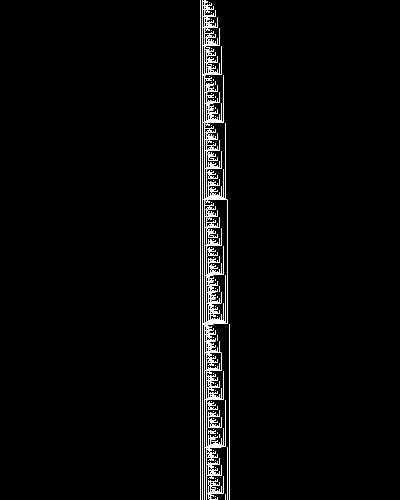
\includegraphics[width=1.1\linewidth]{figures/space-time-diagrams/counter_wfar.png}

        % \vspace{0.8em}
        % \raggedright
        % (a') Space-time diagram \\
        % \vspace{0.3em}
        % \centering
        % 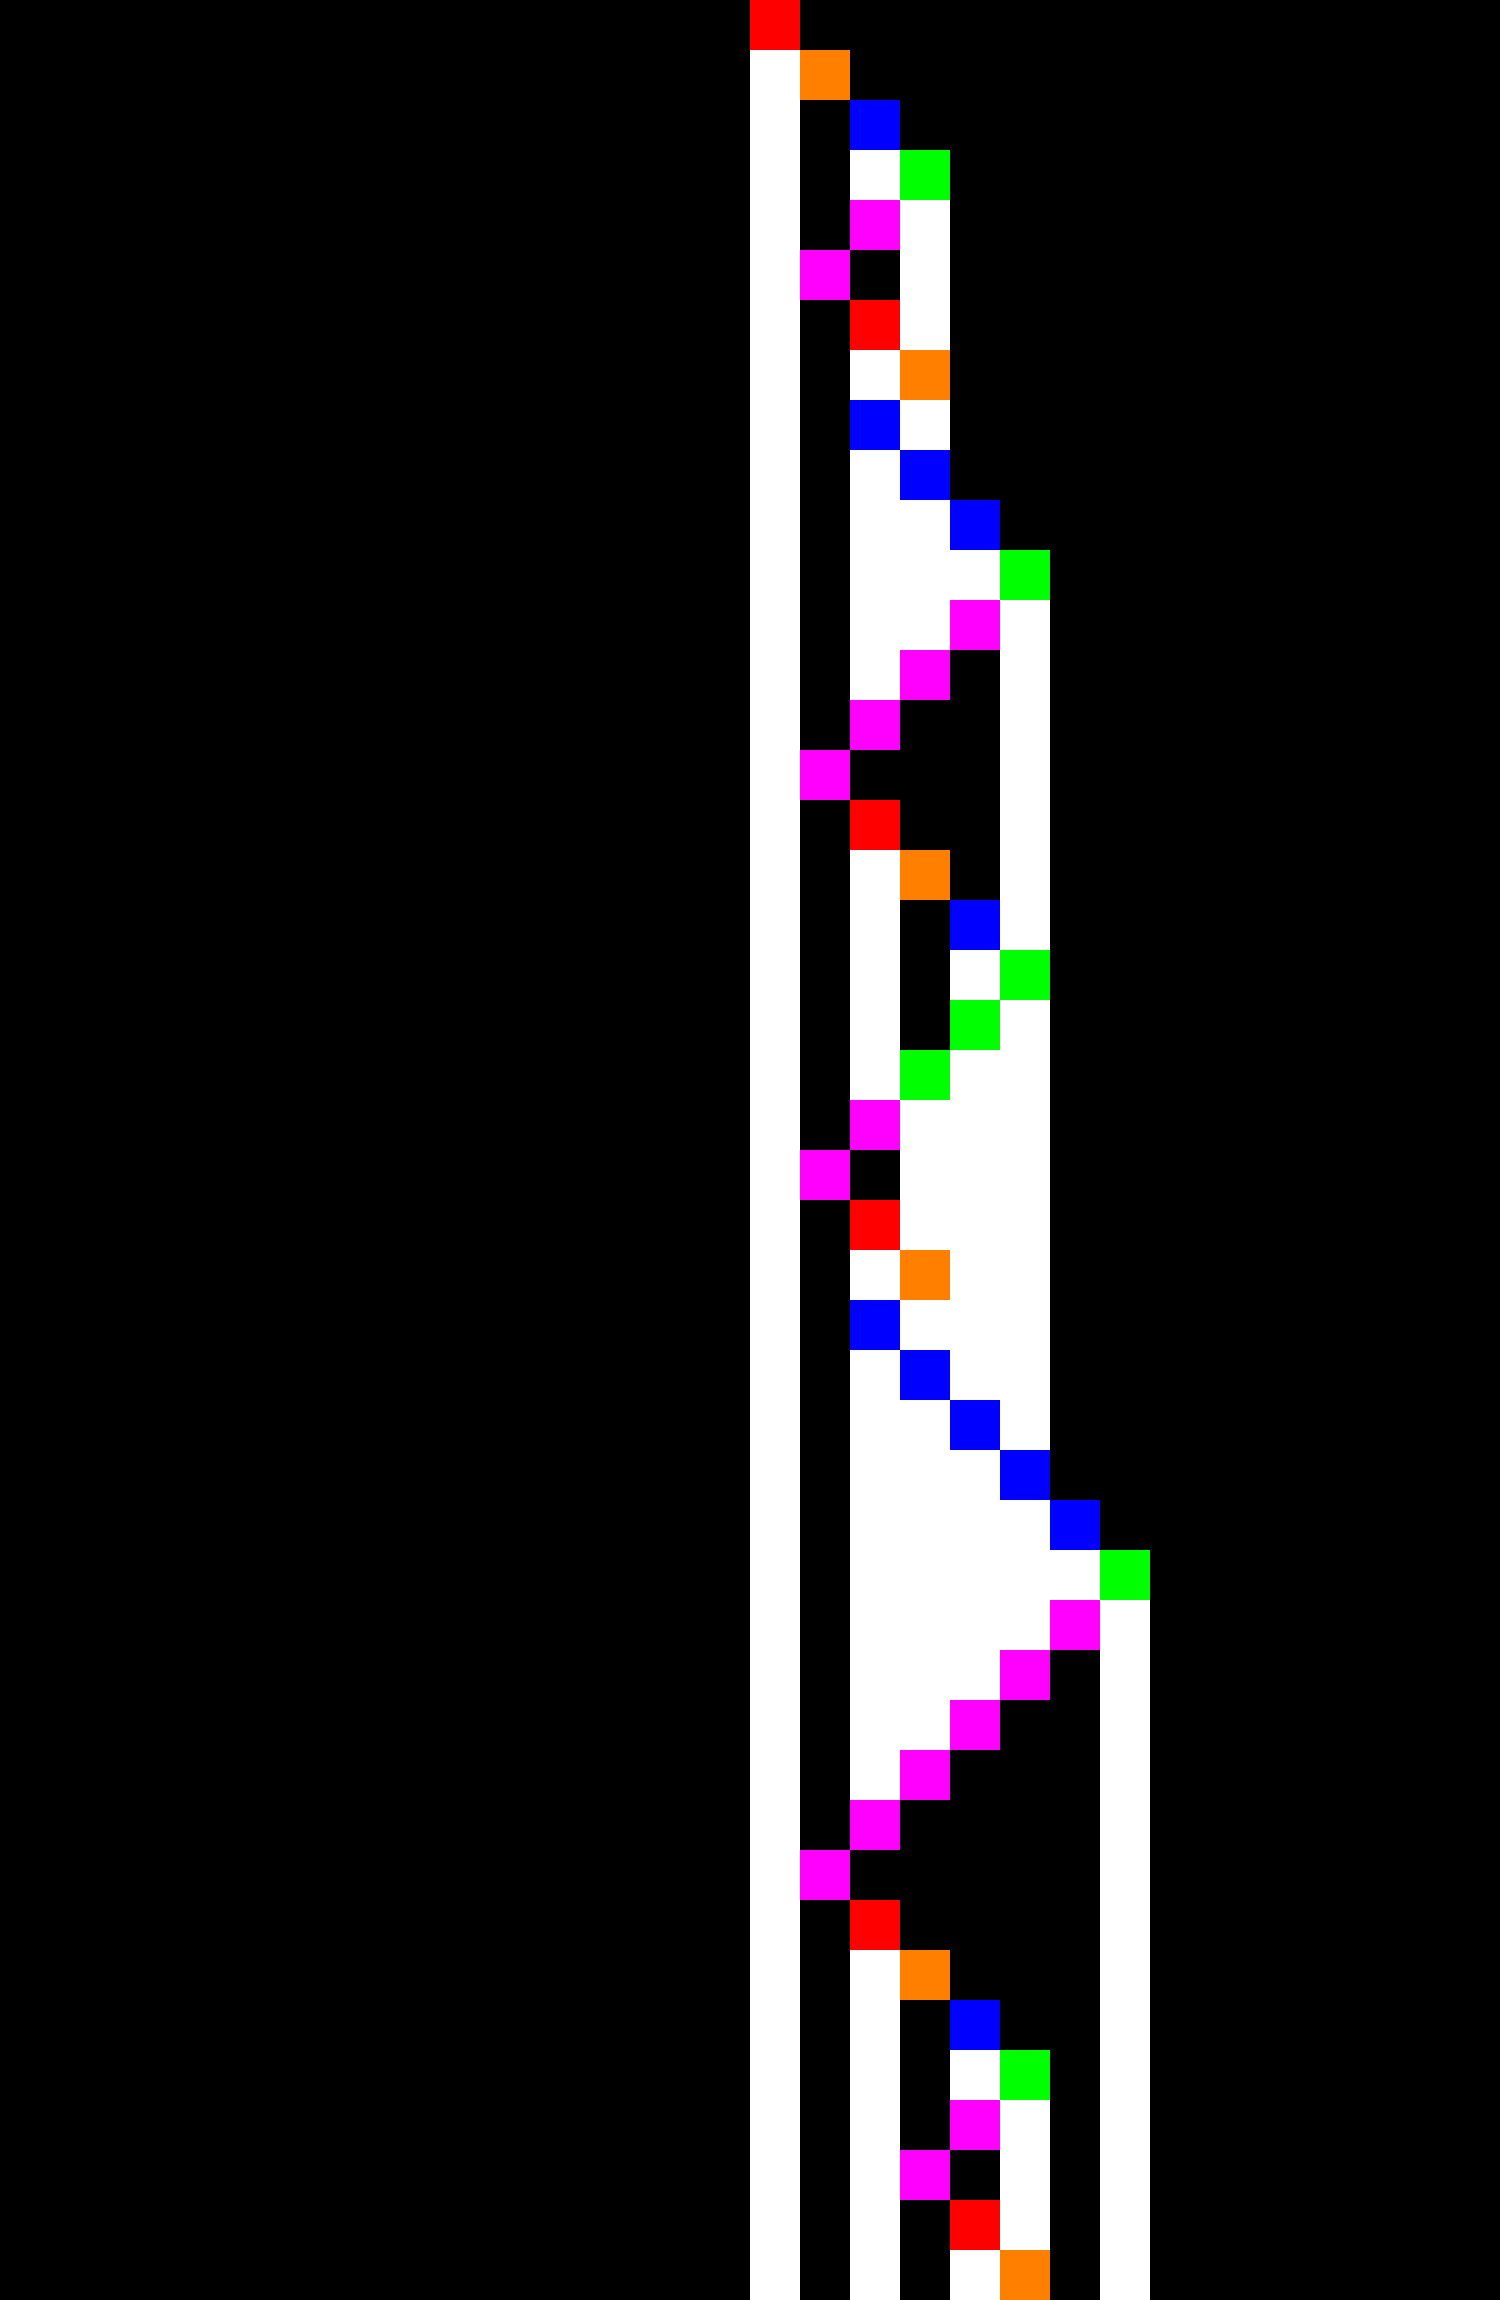
\includegraphics[width=1.1\linewidth]{figures/wfar/wfar_example.pdf}
    \end{minipage}
    \hfill
    \vrule
    \hfill
    \begin{minipage}[t]{0.71\textwidth}

        \begin{minipage}[t]{1\linewidth}

            \begin{minipage}[t]{0.49\textwidth}
                \raggedright
                (b) Left Weighted Automaton \\
                \vspace{0.5em}
                \centering
                \begin{tikzpicture}[->, >=Stealth, auto, node distance=1.8cm, every node/.style={scale=1}]
                    \tikzset{
                        state/.style={
                                circle, draw, minimum size=0.9cm, inner sep=1pt
                            }
                    }

                    % States
                    \node[state] (0) {$p_0$};
                    \node[state] (2) [right of=0] {$p_2$};
                    \node[state] (3) [right of=2] {$p_3$};
                    \node[state] (1) [above of=3] {$p_1$};

                    % Initial arrow
                    \draw[->] (-1,0) -- (0);

                    % Transitions
                    \draw[->, black] (0) edge[loop above] node{\szero} (0);
                    \draw[->, black] (0) edge node{\sone} (2);

                    \draw[->, black] (2) edge[loop above] node{\sone} (2);
                    \draw[->, black, bend left=20] (3) to node{\sone} (2);
                    \draw[->, green!70!black, thick, bend left=20] (2) to node{\szero} (3);

                    \draw[->, black] (3) edge node{\szero} (1);
                    \draw[->, black] (1) edge[loop left] node{\szero, \sone} (1);


                \end{tikzpicture}
            \end{minipage}
            \hfill
            \begin{minipage}[t]{0.49\textwidth}
                \raggedright
                (c) Right Weighted Automaton \\
                \vspace{0.3em}
                \centering
                \begin{tikzpicture}[->, >=Stealth, auto, node distance=2cm, every node/.style={scale=1}]
                    \tikzset{
                        state/.style={
                                circle, draw, minimum size=1cm, inner sep=1pt
                            }
                    }

                    % % Upper isolated state
                    % \node[state] (1top) at (0,2.5) {1};
                    % \draw[->] (1top) edge[loop above] node{1} (1top);
                    % \draw[->] (1top) edge[loop left] node{0} (1top);

                    % Lower automaton
                    \node[state] (0) at (0,0) {$q_0$};
                    \node[state] (2) at (3,0) {
                        $q_1$};

                    \draw[->] (0) edge[loop above] node{\szero} (0);
                    \draw[->] (2) edge[loop above] node{\sone} (2);

                    \draw[->] (0) edge[bend left=10] node{\sone} (2);
                    \draw[->, red, bend left=20, thick] (2) to node[below]{\szero} (0);

                    % Initial state arrow
                    \draw[->] (-1,0) -- (0);

                    % Compact and aligned legend
                    \node[draw, below=0.5cm of 2, inner sep=3pt, rounded corners] (legend) {
                        \scalebox{0.7}{
                            \begin{tabular}{@{}rl@{}}
                                \tikz[baseline=-0.5ex]\draw[->, black, thick] (0,0) -- +(0.6,0);          & \;Weight 0    \\
                                \tikz[baseline=-0.5ex]\draw[->, green!70!black, thick] (0,0) -- +(0.6,0); & \;Weight 1    \\
                                \tikz[baseline=-0.5ex]\draw[->, red, thick] (0,0) -- +(0.6,0);            & \;Weight $-1$
                            \end{tabular}
                        }
                    };
                \end{tikzpicture}
            \end{minipage}

            % \vspace{1em}
            % $\rightarrow$ \quad 1\,0\,|\,0\,|\,0\,1 \\
            % \vspace{0.5em}
            % $+\;4$

        \end{minipage}

        \vspace{1em}

        \raggedright
        (d) Example: configuration is accepted, hence nonhalting \\
        \vspace{0.3em}
        \centering

        \newcommand{\underarrowleft}[1]{%
            \tikz[baseline=(X.base)]{
                \node (X) {$#1$};
                \draw[->, thick] ([yshift=-1.3ex]X.east) -- ([yshift=-1.3ex]X.west);
            }
        }

        \newcommand{\underarrowright}[1]{%
            \tikz[baseline=(X.base)]{
                \node (X) {$#1$};
                \draw[->, thick] ([yshift=-1.3ex]X.west) -- ([yshift=-1.3ex]X.east);
            }
        }

        \scalebox{0.8}{

            \begin{minipage}{\textwidth}
                \centering
                {\LARGE
                $\underarrowright{\texttt{10101}}\; \texttt{\stateC}\sone\; \underarrowleft{\texttt{01}}$ \\
                \vspace{-0.3em}
                {\small $\quad\quad$Left WA reads$\quad\quad\quad\quad\quad\quad\quad\quad$Right WA reads} \\
                %\vspace{0.1em}
                $\quad  \; \;$\fcolorbox{red}{yellow!30}{$[p_2] \; \texttt{\stateC}\sone\; [q_0]$} \\
                \vspace{-2em}
                \[
                    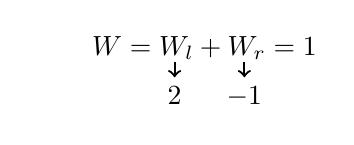
\begin{tikzpicture}[baseline=(base)]
                        \node (base) {$\quad \quad W = W_l + W_r = 1$};

                        \coordinate (Wl) at ([xshift=5.33em]base.base west);
                        \coordinate (Wr) at ([xshift=7.85em]base.base west);

                        % Labels
                        \node[below=1.8ex of Wl] (lval) {\normalsize 2};
                        \node[below=1.8ex of Wr] (rval) {\normalsize $-1$};

                        % Arrows pointing down from W_l and W_r
                        \draw[->, thick] ([yshift=-0.5ex]Wl) -- (lval.north);
                        \draw[->, thick] ([yshift=-0.5ex]Wr) -- (rval.north);
                    \end{tikzpicture}
                \] \\
                \vspace{-0.5em}
                {\large Configuration accepted, see (e), hence machine does not halt starting from $\texttt{10101}\; \texttt{\stateC}\sone\; \texttt{01}$, see Theorem~\ref{th:WFAR}. }
                }
                % \begin{tikzpicture}[->, >=Stealth, auto, node distance=2cm, every node/.style={scale=1}]
                %     \tikzset{
                %         state/.style={
                %                 circle, draw, minimum size=1cm, inner sep=1pt
                %             }
                %     }

                %     % % Upper isolated state
                %     % \node[state] (1top) at (0,2.5) {1};
                %     % \draw[->] (1top) edge[loop above] node{1} (1top);
                %     % \draw[->] (1top) edge[loop left] node{0} (1top);

                %     % Lower automaton
                %     \node[state] (0) at (0,0) {0};
                %     \node[state] (2) at (3,0) {1};

                %     \draw[->] (0) edge[loop above] node{0} (0);
                %     \draw[->] (2) edge[loop above] node{1} (2);

                %     \draw[->] (0) edge[bend left=10] node{1} (2);
                %     \draw[->, red, bend left=20, thick] (2) to node[below]{0} (0);

                %     % Initial state arrow
                %     \draw[->] (-1,0) -- (0);
                % \end{tikzpicture}
            \end{minipage}
        }

        \vspace{0.5em}
        \raggedright
        (e) Accepted weighted configurations \\
        \centering

        \usetikzlibrary{positioning, shapes.multipart, fit}
        \scalebox{0.8}{
            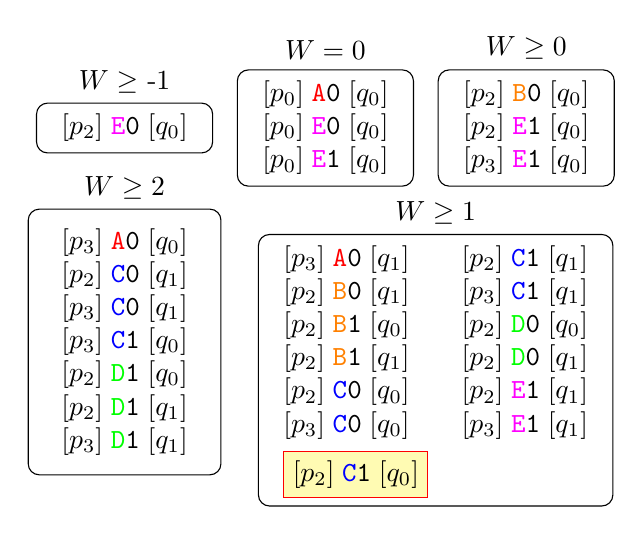
\begin{tikzpicture}[node distance=0.2cm and 0.3cm, every node/.style={font=\normalsize}, anchor=north]

                % Reference coordinate for top alignment
                \coordinate (topref) at (0,0);

                % W >= -1 group
                \node[draw, rectangle, rounded corners, inner sep=3pt] (wmin1box)
                {\begin{tabular}{l}
                        $[p_2]\; \texttt{\stateE}\szero\; [q_0]$
                    \end{tabular}};
                \node[above=0cm of wmin1box] {$W \geq$ -1};

                % W = 0 group
                \node[draw, rectangle, rounded corners, inner sep=3pt, right=of wmin1box] (w0box)
                {\begin{tabular}{l}
                        $[p_0]\; \texttt{\stateA}\szero\; [q_0]$ \\
                        $[p_0]\; \texttt{\stateE}\szero\; [q_0]$ \\
                        $[p_0]\; \texttt{\stateE}\sone\; [q_0]$
                    \end{tabular}};
                \node[above=0cm of w0box] {$W = 0$};

                % W >= 0 group
                \node[draw, rectangle, rounded corners, inner sep=3pt, right=of w0box] (w0plusbox)
                {\begin{tabular}{l}
                        $[p_2]\; \texttt{\stateB}\szero\; [q_0]$ \\
                        $[p_2]\; \texttt{\stateE}\sone\; [q_0]$  \\
                        $[p_3]\; \texttt{\stateE}\sone\; [q_0]$
                    \end{tabular}};
                \node[above=0cm of w0plusbox] {$W\geq0$};
                % W >= 1 group
                \node[draw, rectangle, rounded corners, inner sep=3pt, below=0.6cm of w0box, xshift=1.4cm] (w1box)
                {\begin{tabular}{ll}
                        $[p_3]\; \texttt{\stateA}\szero\; [q_1]$                                             & $[p_2]\; \texttt{\stateC}\sone\; [q_1]$  \\
                        $[p_2]\; \texttt{\stateB}\szero\; [q_1]$                                             & $[p_3]\; \texttt{\stateC}\sone\; [q_1]$  \\
                        $[p_2]\; \texttt{\stateB}\sone\; [q_0]$                                              & $[p_2]\; \texttt{\stateD}\szero\; [q_0]$ \\
                        $[p_2]\; \texttt{\stateB}\sone\; [q_1]$                                              & $[p_2]\; \texttt{\stateD}\szero\; [q_1]$ \\
                        $[p_2]\; \texttt{\stateC}\szero\; [q_0]$                                             & $[p_2]\; \texttt{\stateE}\sone\; [q_1]$  \\
                        $[p_3]\; \texttt{\stateC}\szero\; [q_0]$                                             & $[p_3]\; \texttt{\stateE}\sone\; [q_1]$  \\
                        \rule{0pt}{3.3ex}\fcolorbox{red}{yellow!30}{$[p_2]\; \texttt{\stateC}\sone\; [q_0]$} &                                          \\
                    \end{tabular}};
                \node[above=0cm of w1box] {$W \geq 1$};

                % W >= 2 group
                \node[draw, rectangle, rounded corners, inner sep=6pt, below=0.7cm of wmin1box] (w2box)
                {\begin{tabular}{l}
                        $[p_3]\; \texttt{\stateA}\szero\; [q_0]$ \\
                        $[p_2]\; \texttt{\stateC}\szero\; [q_1]$ \\
                        $[p_3]\; \texttt{\stateC}\szero\; [q_1]$ \\
                        $[p_3]\; \texttt{\stateC}\sone\; [q_0]$  \\
                        $[p_2]\; \texttt{\stateD}\sone\; [q_0]$  \\
                        $[p_2]\; \texttt{\stateD}\sone\; [q_1]$  \\
                        $[p_3]\; \texttt{\stateD}\sone\; [q_1]$  \\
                    \end{tabular}};
                \node[above=0cm of w2box] {$W \geq 2$};

            \end{tikzpicture}
        }
    \end{minipage}

    \caption{{\small WFAR certificate of nonhalting for machine \tm{1RB---_0RC1LC_1RD1RC_1LE1LD_0RA0LE}: (a) transition table and 20,000-step space-time diagram, (b) left weighted automaton: processes symbols to the left of the head in the left-to-right direction, which results in a left end-state -- \eg state $p_2$ when processing \texttt{10101} -- and a left weight obtained by summing the weights of each transition -- \eg $W_l = 2$ when processing \texttt{10101} (c) right weighted automaton: processes symbols to the right of the head (excluding the symbol read by the head) in the right-to-left direction -- indicated with arrow --, which results in a right end-state -- \eg state $q_0$ when processing \texttt{01} right-to-left -- and a right weight -- \eg $W_r = -1$ when processing \texttt{01} right-to-left (d) example, the total weight of configuration $\texttt{10101}\; \texttt{\stateC}\sone\; \texttt{01}$ is $W=W_l+W_r = 1$, using same word-encoding of configurations as in Section~\ref{sec:FAR}, and the right and left end-states are $p_2$ and $q_0$. Weighted automaton configuration $[p_2]\; \texttt{\stateC}\texttt{1}\; [q_0]$ with $W = 1$ is in the set of accepted weighted configurations (under more general $W \geq 1$), see (e). Therefore we know that the machine does not halt from configuration $\texttt{10101}\; \texttt{\stateC}\sone\; \texttt{01}$, Theorem~\ref{th:WFAR}. Similarly, Turing machine configuration $\texttt{\stateA}\texttt{0}$, which results in weighted configuration $[p_0]\;\texttt{\stateA}\texttt{0}\; [q_0]$ with $W=0$ is accepted, ensuring that the machine does not halt from the all-0 initial tape, Theorem~\ref{th:WFAR}.}}\label{fig:WFAR}
\end{figure}

\subsubsection{Overview}\label{sec:WFAR:overview}



\begin{figure}
    \centering
    \begin{tikzpicture}[->, >=Stealth, auto, node distance=2cm, every node/.style={scale=1}]
        \tikzset{
            state/.style={
                    circle, draw, minimum size=1cm, inner sep=1pt
                }
        }

        % % Upper isolated state
        % \node[state] (1top) at (0,2.5) {1};
        % \draw[->] (1top) edge[loop above] node{1} (1top);
        % \draw[->] (1top) edge[loop left] node{0} (1top);

        % Lower automaton
        \node[state] (0) at (0,0) {$q_0$};
        \node[state] (2) at (3,0) {$q_1$};
        \node[state] (3) at (6,0) {$q_2$};

        \draw[->, green!70!black, thick] (0) edge[loop above] node{\szero} (0);
        \draw[->, red, thick] (2) edge[loop above] node{\sone} (2);
        \draw[->] (3) edge[loop above] node{\szero,\sone} (3);

        \draw[->, red, thick] (0) edge[bend left=10] node{\sone} (2);
        \draw[->] (2) to node[below]{\szero} (3);

        % Initial state arrow
        \draw[->] (-1,0) -- (0);

        % Compact and aligned legend
        \node[draw, right=0.5cm of 3, inner sep=3pt, rounded corners] (legend) {
            \scalebox{0.7}{
                \begin{tabular}{@{}rl@{}}
                    \tikz[baseline=-0.5ex]\draw[->, black, thick] (0,0) -- +(0.6,0);          & \;Weight 0    \\
                    \tikz[baseline=-0.5ex]\draw[->, green!70!black, thick] (0,0) -- +(0.6,0); & \;Weight 1    \\
                    \tikz[baseline=-0.5ex]\draw[->, red, thick] (0,0) -- +(0.6,0);            & \;Weight $-1$
                \end{tabular}
            }
        };
    \end{tikzpicture}
    \caption{Weighted automaton recognising nonregular language $\texttt{0}^n \texttt{1}^n$, using accept set $\{(q_1,W=0)\}$ or $\{(q_1,W=0), (q_0,W=0)\}$ if we include the empty word.}\label{fig:ex_wa}
\end{figure}

Weighted automata are an extension of usual finite state automata where each transition is given a weight in $\Z$: when a word is processed, total weight $W \in \Z$ is computed by summing the weights of all the encountered transitions. Accepted words are described by a set of pairs of final-state and weigth lower and upper bounds (potentially infinite) to satisfy: for instance, the archetypal nonregular language $\texttt{0}^n \texttt{1}^n$ is recognised by the weighted automaton of Figure~\ref{fig:ex_wa} using accept set $\{(q_1,0 \leq W \leq 0)\}$ which we can simplify as $\{(q_1,W=0)\}$ and we may add $(q_0,W=0)$ to the set if we want to include the empty word.

Weighted Finite Automata Reduction (WFAR) is an extension of FAR (Section~\ref{sec:FAR}) using deterministic weighted finite automata. Figure~\ref{fig:WFAR} gives a \textit{WFAR automaton}, which is a certificate of nonhalting the machine given in Figure~\ref{fig:WFAR}~(a). A WFAR automaton consists of (i) a \textit{left deterministic weighted automaton} (ii) a \textit{right deterministic weighted automaton} and (iii) a set of accepted \textit{weighted configurations}, see Figure~\ref{fig:WFAR}~(b), (c), and (e).
A WFAR automaton processes word-representations (as defined in Section~\ref{sec:FAR}) of Turing machine configurations\footnote{With finitely many $\sone$s, which we always assume from now on.} in the way describe below, and, if a configuration is accepted by the WFAR automaton, we know that the associated Turing machine does not halt from that configuration, Theorem~\ref{th:WFAR}. That way, WFAR is a CTL method (instead of co-CTL for FAR), see Section~\ref{sec:deciders-overview}. The WFAR automaton of Figure~\ref{fig:WFAR} accepts (see below for what it means) the initial configuration $\texttt{\stateA}\szero$, giving a certificate of nonhalting for the machine of Figure~\ref{fig:WFAR}~(a) from the all-0 tape.

The method was initially developed by Iijil as a decider \cite{iijil1_2025_14914502} and integrated to \CoqBB by mxdys as a verifier: similarly to FAR (Section~\ref{sec:FAR}), 17 WFAR certificates are directly hardcoded in the \Coq proof, see file \texttt{Verifier\_WFAR\_Hardcoded\_Certificates.v}, see Section~\ref{sec:WFAR:results} for results.

\paragraph{WFAR processing.} Let's describe how a WFAR automaton processes a word-represented Turing machine configuration in order to decider whether it is accepted or not, as illustrated in Figure~\ref{fig:WFAR}. WFAR is an extension of the ``Meet-in-the-middle''\footnote{See Section 6.6 in \cite{bbchallengePart1}.} instance of FAR \cite{bbchallengePart1}: word-representations of configurations are split into three segments, (i) word to the left of the head, (ii) head state and symbol, (iii) word to the right of the head; \eg $\texttt{10101}\; \texttt{\stateC}\sone\; \texttt{01}$, Figure~\ref{fig:WFAR}~(d). The left word -- here $\texttt{10101}$ -- is processed left-to-right by the left weighted automaton, Figure~\ref{fig:WFAR}~(b), and the right word -- here $\texttt{01}$ -- is processed right-to-left, by the right weighted automaton, Figure~\ref{fig:WFAR}~(c). In this case, this results in final left state $p_2$, final right state $q_0$, final left weight $W_l = 2$ and final right weight $W_r = -1$; the final total weight is $W = W_l + W_r = 1$, Figure~\ref{fig:WFAR}~(d). We denote this final \textit{weighted configuration} as $[p_2]\; \texttt{\stateC}\sone\; [q_0]$ with $W=1$. This final weighted configuration belongs to the set of accepted weighted configurations, Figure~\ref{fig:WFAR}~(e), which means that configuration $\texttt{10101}\; \texttt{\stateC}\sone\; \texttt{01}$ is \textit{accepted} by this WFAR automaton.


\subsubsection{WFAR theorem}

WFAR is CTL technique -- see Section~\ref{sec:deciders-overview}: a WFAR automaton for a given Turing machine is meant to recognise a language of configurations $\mathcal{L}$ that includes the initial all-0 configuration, closed under Turing machine steps and that does not contain any halting configuration. Hence, we get the following CTL formalism, plus leading/trailing zeros conditions similarly to FAR:
\begin{align}
    u \in \mathcal{L}                               & \iff 0u \in \mathcal{L}               &  & \text{(leading zeros ignored)}
    \tag{\ref{eq:lzignore}}
    \\
    u \in \mathcal{L}                               & \iff u0 \in \mathcal{L}               &  & \text{(trailing zeros ignored)}
    \tag{\ref{eq:tzignore}}
    \\
    c\TMstep\bot                                    & \implies \hat{c} \not \in \mathcal{L} &  & \text{(reject halt)} \label{eq:rejecthalt}     \\
    (c_1\TMstep c_2)\land \hat{c}_1 \in \mathcal{L} & \implies\hat{c}_2 \in \mathcal{L}     &  & \text{(forward closure)} \label{eq:forwardclo}
\end{align}

Let's now show how to verify that a given WFAR automaton for a given Turing machine $\mathcal{M}$ accepts such $\mathcal{L}$, hence providing a certificate that $\mathcal{M}$ does not halt from the all-0 tape.

In the following, $\delta_L: Q_L \times \balphabet \to Q_L$ and $\delta_R: Q_R \times \balphabet \to Q_R$ respectively refer to the transition functions of the deterministic left and right weighted automaton of a WFAR automaton, \eg Figure~\ref{fig:WFAR}~(b) and (c), with $Q_L = \{p_0, \, \dots, \, p_{n_L-1}\}$ and $Q_R = \{q_0, \, \dots, \, q_{n_R-1}\}$ their respective set of states with $n_L$ and $n_R$ the number of left/right states and $p_0$ and $q_0$ are the respective initial states of the left and right weighted automaton. Weights are given by $w_L: Q_L \times \balphabet \to \Z$ and $w_R: Q_R \times \balphabet \to \Z$. We write $\delta_\mathcal{M}:\states \times \balphabet \hookrightarrow \balphabet \times \{\text{L},\text{R}\} \times \states$ for the transition function of $\mathcal{M}$\footnote{In the following, we limit ourselves to the binary tape alphabet $\balphabet$, but the results generalise transparently to arbitrary alphabets $\alphabet$.}.

\paragraph{Leading/trailing zeros.} Checking Conditions~\eqref{eq:lzignore} and \eqref{eq:tzignore} for a WFAR automaton is simple: thanks to the left-to-right and right-to-left respective read directions for the left and right weighted automaton, we simply have to check that $\delta_L(p_0,\szero) = p_0$ and $\delta_R(q_0,\szero) = q_0$ as well as $w_L(p_0,\szero) = w_R(q_0,\szero) = 0$ to ensure the convention that the weight of all word-representations of the initial all-0 configuration is 0.

\paragraph{Forward closure, without weights.} First, let's reformulate forward closure for a WFAR automaton, ignoring weights computations. Forward closure concerns the WFAR automaton's accept state, let's consider an example first. The WFAR automaton of Figure~\ref{fig:WFAR} accepts the initial Turing machine configuration $\texttt{\stateA}\szero$: the WFAR configuration $[p_0] \; \texttt{\stateA}\szero\; [q_0]$ (ignoring $W=0$) is in the accept set given in Figure~\ref{fig:WFAR}~(e). To ensure forward closure, Condition~\ref{eq:forwardclo}, let's consider how $\delta_\mathcal{M}(\texttt{\stateA},\szero) = \texttt{1R\stateB}$ affects $[p_0] \; \texttt{\stateA}\szero\; [q_0]$; we get $[p_0] \; \texttt{1}\; \texttt{\stateB}\texttt{?}\; [\texttt{?}]$, which is $[p_2] \; \texttt{\stateB}\texttt{?}\; [\texttt{?}]$ given that $\delta_L(p_0,\sone) = p_2$, see Figure~\ref{fig:WFAR}~(b). In order to resolve $\texttt{?}$, we look at all the transitions in the right weighted automaton that lead to $q_0$, see Figure~\ref{fig:WFAR}~(c): there are two, both reading a \texttt{0}, giving $[p_2] \; \texttt{\stateB}\texttt{0}\; [q_0]$ and $[p_2] \; \texttt{\stateB}\texttt{0}\; [q_1]$.

Ignoring weights, we want both in the accept set:\footnote{Which is the case here, with $W\geq 0$ and $W \geq 1$ in Figure~\ref{fig:WFAR}~(e).} that ensures that for any Turing machine configuration $c_1$ yielding WFAR configuration $[p_0] \; \texttt{\stateA}\szero\; [q_0]$, then $c_2$ is also accepted by the WFAR automaton with $c_1 \TMstep c_2$. Note that $c_1$ and $c_2$ are not necessarily reachable from the initial all-0 tape: CTL methods provide languages that over-estimate the language generated by Turing machines from the all-0 tape. In general, ignoring weights, forward closure means the following for WFAR automaton accept set $A$:
\begin{align*}
     & \forall q', r' \in Q_R \times \balphabet \text{ s.t. } \delta_R(q', r') = q,
     &                                                                              & [p]\, fr\, [q] \in A \Rightarrow [\delta_L(p,b)]\, tr'\, [q'] \in A
     &                                                                              & \text{if } \delta_{\mathcal{M}}(f,r) = (b, \text{R}, t)
    \\[0.5em]
     & \forall p', r' \in Q_L\times \balphabet \text{ s.t. } \delta_L(p', r') = p,
     &                                                                              & [p]\, fr\, [q] \in A \Rightarrow [p']\, tr'\, [\delta_R(q,b)] \in A
     &                                                                              & \text{if } \delta_{\mathcal{M}}(f,r) = (b, \text{L}, t)
\end{align*}

For all left/right weighted automata states $p,q \in Q_L \times Q_R$ and notations $f,t \in \{\stateA,\stateB,\stateC,\stateD,\stateE\}$ the ``from'' and ``to'' states in a transition, $r,b \in \balphabet$ respectively the bit read and the bit written in a transition.




% Consider Figure~\ref{fig:WFAR}~(d) configuration $c_1 = \texttt{10101}\; \texttt{\stateC}\sone\; \texttt{01}$ which corresponds to WFAR configuration $c'_1 = [p_2] \; \texttt{\stateC}\sone\; [q_0]$ (ignoring weight $W=1$). Applying $\delta_\mathcal{M}(\stateC, \sone) = \texttt{1R\stateC}$ to $c'_1$ gives $[p_2] \; \sone \; \texttt{\stateC}\texttt{?}\; [\texttt{?}]$ which is $[p_2] \; \texttt{\stateC}?\; [?]$ since $\delta_(p_2,\sone) = p_2$. In order to resolve the $\texttt{?}$, we consider all the transitions leading to $q_0$: there are 2, both reading a $\texttt{0}$, see Figure~\ref{fig:WFAR}~(c).


\subsubsection{Implementations and results}\label{sec:WFAR:results}

\newpage
\section{Sporadic 5-state machines}\label{sec:sporadic}

\newpage
\section{Results}\label{sec:sporadic}

\newpage
\section{Zoology}\label{sec:sporadic}


\bibliographystyle{abbrv}
\newpage
\bibliography{bbchallenge-paper}

\appendix

\section{Exact pipelines}\label{app:pipelines}
\section{Lower bounds}\label{app:lowerbounds}
\section{Cryptids}\label{app:cryptids}

\end{document}
